\documentclass{report}

\usepackage[utf8x]{inputenc}
\usepackage{amssymb}
\usepackage{amsthm}
\usepackage{amsmath}
\usepackage{algorithm}
\usepackage{algpseudocode}
\usepackage{color}
\usepackage{multicol}
\usepackage{tikz}
\usepackage{hyperref}
\usepackage{cleveref}
\usepackage{subcaption}
\usepackage{todonotes}
\usepackage{url}
\usepackage{booktabs}
\usepackage{tabularx}
\usepackage{multirow}
\usepackage{pdfpages}
\usetikzlibrary{automata, positioning, chains,fit,shapes}

\tikzset{
diagonal fill/.style 2 args={fill=#2, path picture={
\fill[#1, sharp corners] (path picture bounding box.south west) -|
                         (path picture bounding box.north east) -- cycle;}},
reversed diagonal fill/.style 2 args={fill=#2, path picture={
\fill[#1, sharp corners] (path picture bounding box.north west) |- 
                         (path picture bounding box.south east) -- cycle;}}
}

\definecolor{keywordcolor}{rgb}{0.7, 0.1, 0.1}   % red
\definecolor{commentcolor}{rgb}{0.4, 0.4, 0.4}   % grey
\definecolor{symbolcolor}{rgb}{0.0, 0.1, 0.6}    % blue
\definecolor{sortcolor}{rgb}{0.1, 0.5, 0.1}      % green
\usepackage{listings, lstautogobble}
\def\lstlanguagefiles{lstlean.tex}
\lstset{
    language=lean,
    autogobble=true,
    escapeinside={(.}{.)},
}
\newtheorem{definition}{Definition}
\newtheorem{example}{Example}
\newtheorem{theorem}{Theorem}
\newtheorem{lemma}{Lemma}
\newtheorem{fact}{Fact}


% Define a custom counter for contexample
\newcounter{contexample}[example]
\renewcommand{\thecontexample}{\theexample.\arabic{contexample}}

% Define the contexample environment
\newenvironment{contexample}{%
   \refstepcounter{contexample}%
   \begin{example}[continued]%
}{%
   \end{example}%
}

\usepackage{xspace}
\usepackage{xcolor,colortbl}
\definecolor{redhighlights}{HTML}{FFAA66}
\definecolor{lightblue}{HTML}{55AAFF}
\definecolor{lightred}{HTML}{FF5522}
\definecolor{lightpurple}{HTML}{DD77BB}
\definecolor{lightgreen}{HTML}{55FF55}
\definecolor{darkred}{HTML}{CC4411}
\definecolor{darkblue}{HTML}{176FC0}%{1133AA}
\definecolor{nightblue}{HTML}{2010A0}%{1133AA}
\definecolor{alert}{HTML}{176FC0}
\definecolor{darkgreen}{HTML}{36AB14}
\definecolor{strongyellow}{HTML}{FFE219}
\definecolor{devilscss}{HTML}{666666}

\definecolor{leansymbolcolor}{HTML}{2010A0} % mainly debugging; use black to hide
\newcommand{\repoUrl}{https://github.com/knowsys/CertifyingDatalog/blob/develop}
\newcommand{\repoLinkBase}[2]{\href{\repoUrl/#1}{\textcolor{leansymbolcolor}{\texttt{#2}}}\xspace}
\newcommand{\repoLinkCode}[2]{\repoLinkBase{CertifyingDatalog/#1}{#2}}
\newcommand{\ListtoSet}{\repoLinkCode{Basic.lean\#L5}{List.toSet}}
\newcommand{\ListtoSetmem}{\repoLinkCode{Basic.lean\#L10}{List.toSet\_mem}}
\newcommand{\Listmapexceptunit}{\repoLinkCode{Basic.lean\#L20}{List.map\_except\_unit}}
\newcommand{\ListmapexceptunitIsUnitIffAll}{\repoLinkCode{Basic.lean\#L28}{List.map\_except\_unitIsUnitIffAll}}
\newcommand{\ListeraseAll}{\repoLinkCode{Basic.lean\#L45}{List.eraseAll}}
\newcommand{\ListmemeraseAll}{\repoLinkCode{Basic.lean\#L53}{List.mem\_eraseAll}}
\newcommand{\Listmapexceptgo}{\repoLinkCode{Basic.lean\#L174}{List.map\_except.go}}
\newcommand{\Listmapexcept}{\repoLinkCode{Basic.lean\#L184}{List.map\_except}}
\newcommand{\Listmapexceptgooklength}{\repoLinkCode{Basic.lean\#L186}{List.map\_except\_go\_ok\_length}}
\newcommand{\Listfoldlunion}{\repoLinkCode{Basic.lean\#L208}{List.foldl\_union}}
\newcommand{\Listmemfoldlunion}{\repoLinkCode{Basic.lean\#L210}{List.mem\_foldl\_union}}
\newcommand{\Listsubsetfoldlunion}{\repoLinkCode{Basic.lean\#L222}{List.subset\_foldl\_union}}
\newcommand{\Listsubsetresultfoldlunion}{\repoLinkCode{Basic.lean\#L239}{List.subset\_result\_foldl\_union}}
\newcommand{\Listfoldlunionempty}{\repoLinkCode{Basic.lean\#L262}{List.foldl\_union\_empty}}
\newcommand{\Listfoldlunionsubsetset}{\repoLinkCode{Basic.lean\#L273}{List.foldl\_union\_subset\_set}}
\newcommand{\Finsetfilternc}{\repoLinkCode{Basic.lean\#L286}{Finset.filter\_nc}}
\newcommand{\Finsetmemfilternc}{\repoLinkCode{Basic.lean\#L288}{Finset.mem\_filter\_nc}}
\newcommand{\partialGroundRule}{\repoLinkCode{ModelChecking.lean\#L7}{partialGroundRule}}
\newcommand{\partialGroundRuleisSafe}{\repoLinkCode{ModelChecking.lean\#L14}{partialGroundRule.isSafe}}
\newcommand{\partialGroundRulefromRule}{\repoLinkCode{ModelChecking.lean\#L17}{partialGroundRule.fromRule}}
\newcommand{\partialGroundRuletoRule}{\repoLinkCode{ModelChecking.lean\#L20}{partialGroundRule.toRule}}
\newcommand{\partialGroundRuleToRuleInverseToFromRule}{\repoLinkCode{ModelChecking.lean\#L23}{partialGroundRuleToRuleInverseToFromRule}}
\newcommand{\partialGroundRuleisActive}{\repoLinkCode{ModelChecking.lean\#L28}{partialGroundRule.isActive}}
\newcommand{\partialGroundRulefromRuleIsActive}{\repoLinkCode{ModelChecking.lean\#L31}{partialGroundRule.fromRuleIsActive}}
\newcommand{\partialGroundRuleisTrue}{\repoLinkCode{ModelChecking.lean\#L36}{partialGroundRule.isTrue}}
\newcommand{\partialGroundRuleisTrueofequaltoRule}{\repoLinkCode{ModelChecking.lean\#L38}{partialGroundRule.isTrue\_of\_equal\_toRule}}
\newcommand{\atomGroundingOnGroundAtomReturnsSame}{\repoLinkCode{ModelChecking.lean\#L48}{atomGroundingOnGroundAtomReturnsSame}}
\newcommand{\groundingOnPartialGroundRule}{\repoLinkCode{ModelChecking.lean\#L64}{groundingOnPartialGroundRule}}
\newcommand{\notActiveRuleIsTrue}{\repoLinkCode{ModelChecking.lean\#L76}{notActiveRuleIsTrue}}
\newcommand{\getSubstitutions}{\repoLinkCode{ModelChecking.lean\#L96}{getSubstitutions}}
\newcommand{\groundAtomsHaveNoVariables}{\repoLinkCode{ModelChecking.lean\#L98}{groundAtomsHaveNoVariables}}
\newcommand{\inGetSubstitutionsImplNoVars}{\repoLinkCode{ModelChecking.lean\#L111}{inGetSubstitutionsImplNoVars}}
\newcommand{\atomWithoutVariablesToGroundAtomOfGroundAtom}{\repoLinkCode{ModelChecking.lean\#L128}{atomWithoutVariablesToGroundAtomOfGroundAtom}}
\newcommand{\groundingAtomWithoutVariablesYieldsSelf}{\repoLinkCode{ModelChecking.lean\#L144}{groundingAtomWithoutVariablesYieldsSelf}}
\newcommand{\inGetSubstitutionsImplInInterpretation}{\repoLinkCode{ModelChecking.lean\#L174}{inGetSubstitutionsImplInInterpretation}}
\newcommand{\inGetSubstitutionsIffMinimalSolutionAndInInterpretation}{\repoLinkCode{ModelChecking.lean\#L196}{inGetSubstitutionsIffMinimalSolutionAndInInterpretation}}
\newcommand{\headOfSafePgrWithoutGroundedBodyHasNoVariables}{\repoLinkCode{ModelChecking.lean\#L268}{headOfSafePgrWithoutGroundedBodyHasNoVariables}}
\newcommand{\moveAtomWithoutVariables}{\repoLinkCode{ModelChecking.lean\#L278}{moveAtomWithoutVariables}}
\newcommand{\moveAtomWithoutVariablesPreservesSafety}{\repoLinkCode{ModelChecking.lean\#L285}{moveAtomWithoutVariablesPreservesSafety}}
\newcommand{\groundingStep}{\repoLinkCode{ModelChecking.lean\#L298}{groundingStep}}
\newcommand{\groundingStepPreservesSafety}{\repoLinkCode{ModelChecking.lean\#L305}{groundingStepPreservesSafety}}
\newcommand{\exploreGrounding}{\repoLinkCode{ModelChecking.lean\#L345}{exploreGrounding}}
\newcommand{\applySubstitutionOnConstantIsSame}{\repoLinkCode{ModelChecking.lean\#L377}{applySubstitutionOnConstantIsSame}}
\newcommand{\applySubstitutionOnGroundAtomIsSame}{\repoLinkCode{ModelChecking.lean\#L381}{applySubstitutionOnGroundAtomIsSame}}
\newcommand{\swapPgrApplySubstitution}{\repoLinkCode{ModelChecking.lean\#L394}{swapPgrApplySubstitution}}
\newcommand{\combineSubstitutionGrounding}{\repoLinkCode{ModelChecking.lean\#L410}{combineSubstitutionGrounding}}
\newcommand{\combineSubstitutionGroundingEquivTerm}{\repoLinkCode{ModelChecking.lean\#L412}{combineSubstitutionGroundingEquivTerm}}
\newcommand{\combineSubstitutionGroundingEquivAtom}{\repoLinkCode{ModelChecking.lean\#L424}{combineSubstitutionGroundingEquivAtom}}
\newcommand{\combineSubstitutionGroundingEquivRule}{\repoLinkCode{ModelChecking.lean\#L434}{combineSubstitutionGroundingEquivRule}}
\newcommand{\atomSubOfGrounding}{\repoLinkCode{ModelChecking.lean\#L443}{atomSubOfGrounding}}
\newcommand{\atomSubOfGroundingEqOnTerm}{\repoLinkCode{ModelChecking.lean\#L445}{atomSubOfGroundingEqOnTerm}}
\newcommand{\atomSubOfGroundingEqOnAtom}{\repoLinkCode{ModelChecking.lean\#L473}{atomSubOfGroundingEqOnAtom}}
\newcommand{\equalOfListMapEqual}{\repoLinkCode{ModelChecking.lean\#L486}{equalOfListMapEqual}}
\newcommand{\atomSubOfGroundingIsMinimalForAtom}{\repoLinkCode{ModelChecking.lean\#L502}{atomSubOfGroundingIsMinimalForAtom}}
\newcommand{\atomSubOfGroundingGroundingEqGroundingOnTerm}{\repoLinkCode{ModelChecking.lean\#L555}{atomSubOfGroundingGroundingEqGroundingOnTerm}}
\newcommand{\atomSubOfGroundingGroundingEqGroundingOnAtom}{\repoLinkCode{ModelChecking.lean\#L572}{atomSubOfGroundingGroundingEqGroundingOnAtom}}
\newcommand{\atomSubOfGroundingGroundingEqGroundingOnRule}{\repoLinkCode{ModelChecking.lean\#L584}{atomSubOfGroundingGroundingEqGroundingOnRule}}
\newcommand{\replaceGroundingWithSubstitutionAndGrounding}{\repoLinkCode{ModelChecking.lean\#L597}{replaceGroundingWithSubstitutionAndGrounding}}
\newcommand{\exploreGroundingSemantics}{\repoLinkCode{ModelChecking.lean\#L626}{exploreGroundingSemantics}}
\newcommand{\safePreservedBetweenRuleAndPartialGroundRule}{\repoLinkCode{ModelChecking.lean\#L792}{safePreservedBetweenRuleAndPartialGroundRule}}
\newcommand{\modelChecker}{\repoLinkCode{ModelChecking.lean\#L798}{modelChecker}}
\newcommand{\modelCheckerUnitIffAllRulesTrue}{\repoLinkCode{ModelChecking.lean\#L805}{modelCheckerUnitIffAllRulesTrue}}
\newcommand{\signature}{\repoLinkCode{Datalog.lean\#L7}{signature}}
\newcommand{\term}{\repoLinkCode{Datalog.lean\#L18}{term}}
\newcommand{\atom}{\repoLinkCode{Datalog.lean\#L33}{atom}}
\newcommand{\atomEquality}{\repoLinkCode{Datalog.lean\#L47}{atomEquality}}
\newcommand{\datalogrule}{\repoLinkCode{Datalog.lean\#L61}{rule}}
\newcommand{\ruleEquality}{\repoLinkCode{Datalog.lean\#L71}{ruleEquality}}
\newcommand{\program}{\repoLinkCode{Datalog.lean\#L85}{program}}
\newcommand{\groundAtom}{\repoLinkCode{Datalog.lean\#L94}{groundAtom}}
\newcommand{\listMapPreservesTermLength}{\repoLinkCode{Datalog.lean\#L101}{listMapPreservesTermLength}}
\newcommand{\groundAtomEquality}{\repoLinkCode{Datalog.lean\#L106}{groundAtomEquality}}
\newcommand{\groundAtomtoAtom}{\repoLinkCode{Datalog.lean\#L119}{groundAtom.toAtom}}
\newcommand{\listMapInjectiveEquality}{\repoLinkCode{Datalog.lean\#L121}{listMapInjectiveEquality}}
\newcommand{\groundAtomToAtomEquality}{\repoLinkCode{Datalog.lean\#L151}{groundAtomToAtomEquality}}
\newcommand{\termVariables}{\repoLinkCode{Datalog.lean\#L173}{termVariables}}
\newcommand{\atomVariables}{\repoLinkCode{Datalog.lean\#L178}{atomVariables}}
\newcommand{\atomVariablesSubsetImpltermVariablesSubset}{\repoLinkCode{Datalog.lean\#L181}{atomVariablesSubsetImpltermVariablesSubset}}
\newcommand{\ruleVariables}{\repoLinkCode{Datalog.lean\#L191}{ruleVariables}}
\newcommand{\ruleVariablesSubsetImplAtomVariablesSubset}{\repoLinkCode{Datalog.lean\#L193}{ruleVariablesSubsetImplAtomVariablesSubset}}
\newcommand{\ruleisSafe}{\repoLinkCode{Datalog.lean\#L214}{rule.isSafe}}
\newcommand{\safetyCheckRule}{\repoLinkCode{Datalog.lean\#L216}{safetyCheckRule}}
\newcommand{\safetyCheckRuleUnitIffRuleSafe}{\repoLinkCode{Datalog.lean\#L223}{safetyCheckRuleUnitIffRuleSafe}}
\newcommand{\safetyCheckProgram}{\repoLinkCode{Datalog.lean\#L238}{safetyCheckProgram}}
\newcommand{\safetyCheckProgramUnitIffProgramSafe}{\repoLinkCode{Datalog.lean\#L241}{safetyCheckProgramUnitIffProgramSafe}}
\newcommand{\groundRule}{\repoLinkCode{Datalog.lean\#L248}{groundRule}}
\newcommand{\groundRuletoRule}{\repoLinkCode{Datalog.lean\#L254}{groundRule.toRule}}
\newcommand{\groundRuletoRulePreservesLength}{\repoLinkCode{Datalog.lean\#L259}{groundRuletoRulePreservesLength}}
\newcommand{\groundRuleEquality}{\repoLinkCode{Datalog.lean\#L268}{groundRuleEquality}}
\newcommand{\groundRuleToRuleEquality}{\repoLinkCode{Datalog.lean\#L281}{groundRuleToRuleEquality}}
\newcommand{\grounding}{\repoLinkCode{Datalog.lean\#L303}{grounding}}
\newcommand{\applyGroundingTerm}{\repoLinkCode{Datalog.lean\#L305}{applyGroundingTerm}}
\newcommand{\applyGroundingTermRemovesVariables}{\repoLinkCode{Datalog.lean\#L310}{applyGroundingTermRemovesVariables}}
\newcommand{\applyGroundingTermPreservesLength}{\repoLinkCode{Datalog.lean\#L322}{applyGroundingTermPreservesLength}}
\newcommand{\applyGroundingAtom}{\repoLinkCode{Datalog.lean\#L329}{applyGroundingAtom}}
\newcommand{\groundingRemovesAtomVariables}{\repoLinkCode{Datalog.lean\#L332}{groundingRemovesAtomVariables}}
\newcommand{\atomGrounding}{\repoLinkCode{Datalog.lean\#L358}{atomGrounding}}
\newcommand{\applyGroundingRule}{\repoLinkCode{Datalog.lean\#L361}{applyGroundingRule}}
\newcommand{\groundingRemovesRuleVariables}{\repoLinkCode{Datalog.lean\#L363}{groundingRemovesRuleVariables}}
\newcommand{\ruleGrounding}{\repoLinkCode{Datalog.lean\#L375}{ruleGrounding}}
\newcommand{\groundRuleBodySet}{\repoLinkCode{Datalog.lean\#L377}{groundRuleBodySet}}
\newcommand{\groundRuleBodySetiffgroundRuleBody}{\repoLinkCode{Datalog.lean\#L379}{groundRuleBodySet\_iff\_groundRuleBody}}
\newcommand{\ruleFromGroundAtoms}{\repoLinkCode{Datalog.lean\#L385}{ruleFromGroundAtoms}}
\newcommand{\groundProgram}{\repoLinkCode{Datalog.lean\#L387}{groundProgram}}
\newcommand{\termWithoutVariablesToConstant}{\repoLinkCode{Datalog.lean\#L389}{termWithoutVariablesToConstant}}
\newcommand{\atomVariablesEmptyIffAllTermVariablesEmpty}{\repoLinkCode{Datalog.lean\#L398}{atomVariablesEmptyIffAllTermVariablesEmpty}}
\newcommand{\atomWithoutVariablesToGroundAtom}{\repoLinkCode{Datalog.lean\#L403}{atomWithoutVariablesToGroundAtom}}
\newcommand{\groundAtomToAtomOfAtomWithoutVariablesToGroundAtomIsSelf}{\repoLinkCode{Datalog.lean\#L413}{groundAtomToAtomOfAtomWithoutVariablesToGroundAtomIsSelf}}
\newcommand{\substitution}{\repoLinkCode{Datalog.lean\#L444}{substitution}}
\newcommand{\substitutiondomain}{\repoLinkCode{Datalog.lean\#L446}{substitution\_domain}}
\newcommand{\applySubstitutionTerm}{\repoLinkCode{Datalog.lean\#L448}{applySubstitutionTerm}}
\newcommand{\applySubstitutionTermMapPreservesLength}{\repoLinkCode{Datalog.lean\#L453}{applySubstitutionTermMapPreservesLength}}
\newcommand{\applySubstitutionAtom}{\repoLinkCode{Datalog.lean\#L458}{applySubstitutionAtom}}
\newcommand{\applySubstitutionRule}{\repoLinkCode{Datalog.lean\#L461}{applySubstitutionRule}}
\newcommand{\VarInDomainIffApplySubstitutionTermIsConst}{\repoLinkCode{Datalog.lean\#L463}{VarInDomainIffApplySubstitutionTermIsConst}}
\newcommand{\applySubstitutionAtomIsGroundImplVarsSubsetDomain}{\repoLinkCode{Datalog.lean\#L488}{applySubstitutionAtomIsGroundImplVarsSubsetDomain}}
\newcommand{\applySubstitutionRuleIsGroundImplVarsSubsetDomain}{\repoLinkCode{Datalog.lean\#L524}{applySubstitutionRuleIsGroundImplVarsSubsetDomain}}
\newcommand{\groundingToSubstitution}{\repoLinkCode{Datalog.lean\#L568}{groundingToSubstitution}}
\newcommand{\groundingToSubsitutionEquivTerm}{\repoLinkCode{Datalog.lean\#L570}{groundingToSubsitutionEquivTerm}}
\newcommand{\groundingToSubsitutionEquivAtom}{\repoLinkCode{Datalog.lean\#L583}{groundingToSubsitutionEquivAtom}}
\newcommand{\groundingToSubsitutionEquivRule}{\repoLinkCode{Datalog.lean\#L602}{groundingToSubsitutionEquivRule}}
\newcommand{\substitutionToGrounding}{\repoLinkCode{Datalog.lean\#L621}{substitutionToGrounding}}
\newcommand{\substitutionToGroundingEquivTerm}{\repoLinkCode{Datalog.lean\#L623}{substitutionToGroundingEquivTerm}}
\newcommand{\substitutionToGroundingEquivAtom}{\repoLinkCode{Datalog.lean\#L643}{substitutionToGroundingEquivAtom}}
\newcommand{\substitutionToGroundingEquivRule}{\repoLinkCode{Datalog.lean\#L660}{substitutionToGroundingEquivRule}}
\newcommand{\groundingSubstitutionEquivalence}{\repoLinkCode{Datalog.lean\#L684}{groundingSubstitutionEquivalence}}
\newcommand{\emptySubstitution}{\repoLinkCode{Datalog.lean\#L703}{emptySubstitution}}
\newcommand{\substitutionsubs}{\repoLinkCode{Datalog.lean\#L705}{substitution\_subs}}
\newcommand{\emptySubstitutionIsMinimal}{\repoLinkCode{Datalog.lean\#L711}{emptySubstitutionIsMinimal}}
\newcommand{\substitutionsubsget}{\repoLinkCode{Datalog.lean\#L720}{substitution\_subs\_get}}
\newcommand{\substitutionsubsnone}{\repoLinkCode{Datalog.lean\#L733}{substitution\_subs\_none}}
\newcommand{\substitutionsubsrefl}{\repoLinkCode{Datalog.lean\#L754}{substitution\_subs\_refl}}
\newcommand{\substitutionsubsantisymm}{\repoLinkCode{Datalog.lean\#L759}{substitution\_subs\_antisymm}}
\newcommand{\substitutionsubstrans}{\repoLinkCode{Datalog.lean\#L770}{substitution\_subs\_trans}}
\newcommand{\optiongetiffeqsome}{\repoLinkCode{Datalog.lean\#L786}{option\_get\_iff\_eq\_some}}
\newcommand{\subsextgroundTerm}{\repoLinkCode{Datalog.lean\#L801}{subs\_ext\_groundTerm}}
\newcommand{\subsextlistConstant}{\repoLinkCode{Datalog.lean\#L823}{subs\_ext\_listConstant}}
\newcommand{\subsextgroundAtom}{\repoLinkCode{Datalog.lean\#L845}{subs\_ext\_groundAtom}}
\newcommand{\termVariablesApplySubstitution}{\repoLinkCode{Datalog.lean\#L856}{termVariablesApplySubstitution}}
\newcommand{\atomVariablesApplySubstitution}{\repoLinkCode{Datalog.lean\#L897}{atomVariablesApplySubstitution}}
\newcommand{\database}{\repoLinkCode{Datalog.lean\#L940}{database}}
\newcommand{\interpretation}{\repoLinkCode{Datalog.lean\#L944}{interpretation}}
\newcommand{\tree}{\repoLinkCode{Datalog.lean\#L947}{tree}}
\newcommand{\proofTree}{\repoLinkCode{Datalog.lean\#L950}{proofTree}}
\newcommand{\member}{\repoLinkCode{Datalog.lean\#L955}{member}}
\newcommand{\elementMember}{\repoLinkCode{Datalog.lean\#L961}{elementMember}}
\newcommand{\proofTreeElements}{\repoLinkCode{Datalog.lean\#L972}{proofTreeElements}}
\newcommand{\foldlappendmem}{\repoLinkCode{Datalog.lean\#L980}{foldl\_append\_mem}}
\newcommand{\treeRoot}{\repoLinkCode{Datalog.lean\#L990}{root}}
\newcommand{\children}{\repoLinkCode{Datalog.lean\#L993}{children}}
\newcommand{\listMax}{\repoLinkCode{Datalog.lean\#L996}{listMax}}
\newcommand{\natListmax}{\repoLinkCode{Datalog.lean\#L1000}{natList\_max}}
\newcommand{\listMaxlefmember}{\repoLinkCode{Datalog.lean\#L1004}{listMax\_le\_f\_member}}
\newcommand{\listMaxiffnatListmaxmap}{\repoLinkCode{Datalog.lean\#L1031}{listMax\_iff\_natList\_max\_map}}
\newcommand{\height}{\repoLinkCode{Datalog.lean\#L1046}{height}}
\newcommand{\heightcase}{\repoLinkCode{Datalog.lean\#L1056}{height\_case}}
\newcommand{\heightOfMemberIsSmaller}{\repoLinkCode{Datalog.lean\#L1062}{heightOfMemberIsSmaller}}
\newcommand{\inProofTreeElementsIffelementMember}{\repoLinkCode{Datalog.lean\#L1072}{inProofTreeElementsIffelementMember}}
\newcommand{\isValid}{\repoLinkCode{Datalog.lean\#L1129}{isValid}}
\newcommand{\databaseElementsHaveValidProofTree}{\repoLinkCode{Datalog.lean\#L1140}{databaseElementsHaveValidProofTree}}
\newcommand{\proofTheoreticSemantics}{\repoLinkCode{Datalog.lean\#L1152}{proofTheoreticSemantics}}
\newcommand{\allTreeElementsOfValidTreeInSemantics}{\repoLinkCode{Datalog.lean\#L1154}{allTreeElementsOfValidTreeInSemantics}}
\newcommand{\ruleTrue}{\repoLinkCode{Datalog.lean\#L1205}{ruleTrue}}
\newcommand{\model}{\repoLinkCode{Datalog.lean\#L1207}{model}}
\newcommand{\getTreeHelper}{\repoLinkCode{Datalog.lean\#L1210}{getTree\_Helper}}
\newcommand{\createProofTreeForRule}{\repoLinkCode{Datalog.lean\#L1252}{createProofTreeForRule}}
\newcommand{\proofTheoreticSemanticsIsModel}{\repoLinkCode{Datalog.lean\#L1287}{proofTheoreticSemanticsIsModel}}
\newcommand{\modelTheoreticSemantics}{\repoLinkCode{Datalog.lean\#L1304}{modelTheoreticSemantics}}
\newcommand{\leastModel}{\repoLinkCode{Datalog.lean\#L1306}{leastModel}}
\newcommand{\modelTheoreticSemanticsIsModel}{\repoLinkCode{Datalog.lean\#L1316}{modelTheoreticSemanticsIsModel}}
\newcommand{\proofTreeAtomsInEveryModel}{\repoLinkCode{Datalog.lean\#L1354}{proofTreeAtomsInEveryModel}}
\newcommand{\SemanticsEquivalence}{\repoLinkCode{Datalog.lean\#L1405}{SemanticsEquivalence}}
\newcommand{\PreGraph}{\repoLinkCode{GraphValidation.lean\#L8}{PreGraph}}
\newcommand{\PreGraphvertices}{\repoLinkCode{GraphValidation.lean\#L13}{vertices}}
\newcommand{\PreGraphsuccessors}{\repoLinkCode{GraphValidation.lean\#L14}{successors}}
\newcommand{\PreGraphcomplete}{\repoLinkCode{GraphValidation.lean\#L16}{complete}}
\newcommand{\PreGraphinverticesiffcontains}{\repoLinkCode{GraphValidation.lean\#L18}{in\_vertices\_iff\_contains}}
\newcommand{\PreGraphinsuccessorsifffound}{\repoLinkCode{GraphValidation.lean\#L19}{in\_successors\_iff\_found}}
\newcommand{\PreGraphfromvertices}{\repoLinkCode{GraphValidation.lean\#L21}{from\_vertices}}
\newcommand{\PreGraphaddvertex}{\repoLinkCode{GraphValidation.lean\#L23}{add\_vertex}}
\newcommand{\PreGraphaddvertices}{\repoLinkCode{GraphValidation.lean\#L35}{add\_vertices}}
\newcommand{\PreGraphaddverticescontainsiffcontainsorinlist}{\repoLinkCode{GraphValidation.lean\#L38}{add\_vertices\_contains\_iff\_contains\_or\_in\_list}}
\newcommand{\PreGraphaddverticesfindDsemantics}{\repoLinkCode{GraphValidation.lean\#L108}{add\_vertices\_findD\_semantics}}
\newcommand{\PreGraphaddvertexwithsuccessors}{\repoLinkCode{GraphValidation.lean\#L121}{add\_vertex\_with\_successors}}
\newcommand{\PreGraphfromverticescontainsexactlythepassedvertices}{\repoLinkCode{GraphValidation.lean\#L125}{from\_vertices\_contains\_exactly\_the\_passed\_vertices}}
\newcommand{\PreGraphfromverticesnovertexhassuccessors}{\repoLinkCode{GraphValidation.lean\#L131}{from\_vertices\_no\_vertex\_has\_successors}}
\newcommand{\PreGraphfromverticesiscomplete}{\repoLinkCode{GraphValidation.lean\#L147}{from\_vertices\_is\_complete}}
\newcommand{\PreGraphaddvertexwithsuccessorscontainsiffcontainsorinnewvertices}{\repoLinkCode{GraphValidation.lean\#L160}{add\_vertex\_with\_successors\_contains\_iff\_contains\_or\_in\_new\_vertices}}
\newcommand{\PreGraphaddvertexwithsuccessorsstillcomplete}{\repoLinkCode{GraphValidation.lean\#L372}{add\_vertex\_with\_successors\_still\_complete}}
\newcommand{\Graph}{\repoLinkCode{GraphValidation.lean\#L421}{Graph}}
\newcommand{\Graphvertices}{\repoLinkCode{GraphValidation.lean\#L426}{vertices}}
\newcommand{\Graphsuccessors}{\repoLinkCode{GraphValidation.lean\#L427}{successors}}
\newcommand{\Graphcomplete}{\repoLinkCode{GraphValidation.lean\#L429}{complete}}
\newcommand{\Graphfromvertices}{\repoLinkCode{GraphValidation.lean\#L439}{from\_vertices}}
\newcommand{\Graphaddvertexwithsuccessors}{\repoLinkCode{GraphValidation.lean\#L451}{add\_vertex\_with\_successors}}
\newcommand{\predlt}{\repoLinkCode{GraphValidation.lean\#L462}{pred\_lt}}
\newcommand{\Natpredgtzeroiff}{\repoLinkCode{GraphValidation.lean\#L474}{Nat.pred\_gt\_zero\_iff}}
\newcommand{\isWalk}{\repoLinkCode{GraphValidation.lean\#L489}{isWalk}}
\newcommand{\isWalkSingleton}{\repoLinkCode{GraphValidation.lean\#L492}{isWalkSingleton}}
\newcommand{\getwoimgtzero}{\repoLinkCode{GraphValidation.lean\#L504}{ge\_two\_im\_gt\_zero}}
\newcommand{\isCycle}{\repoLinkCode{GraphValidation.lean\#L512}{isCycle}}
\newcommand{\IsWalkOfisCycle}{\repoLinkCode{GraphValidation.lean\#L528}{IsWalkOfisCycle}}
\newcommand{\isAcyclic}{\repoLinkCode{GraphValidation.lean\#L537}{isAcyclic}}
\newcommand{\isWalkextendssuccessors}{\repoLinkCode{GraphValidation.lean\#L543}{isWalk\_extends\_successors}}
\newcommand{\isWalkImplSubset}{\repoLinkCode{GraphValidation.lean\#L589}{isWalkImplSubset}}
\newcommand{\isWalkofcons}{\repoLinkCode{GraphValidation.lean\#L603}{isWalk\_of\_cons}}
\newcommand{\getFirstForNonequalisLt}{\repoLinkCode{GraphValidation.lean\#L629}{getFirstForNonequal\_isLt}}
\newcommand{\getLastForNonequalisLt}{\repoLinkCode{GraphValidation.lean\#L635}{getLastForNonequal\_isLt}}
\newcommand{\canReach}{\repoLinkCode{GraphValidation.lean\#L643}{canReach}}
\newcommand{\canReachrefl}{\repoLinkCode{GraphValidation.lean\#L645}{canReach\_refl}}
\newcommand{\globalSuccessors}{\repoLinkCode{GraphValidation.lean\#L669}{globalSuccessors}}
\newcommand{\isWalkExtendBack}{\repoLinkCode{GraphValidation.lean\#L672}{isWalkExtendBack}}
\newcommand{\globalSuccessorsSubsetWhenSuccessor}{\repoLinkCode{GraphValidation.lean\#L714}{globalSuccessorsSubsetWhenSuccessor}}
\newcommand{\nodeNotInGlobalSuccessorOfSuccessorInAcyclic}{\repoLinkCode{GraphValidation.lean\#L746}{nodeNotInGlobalSuccessorOfSuccessorInAcyclic}}
\newcommand{\globalSuccessorsSSubsetWhenAcyclicAndSuccessor}{\repoLinkCode{GraphValidation.lean\#L789}{globalSuccessorsSSubsetWhenAcyclicAndSuccessor}}
\newcommand{\removeFrontOfLtMin}{\repoLinkCode{GraphValidation.lean\#L824}{removeFrontOfLtMin}}
\newcommand{\getSubListToMember}{\repoLinkCode{GraphValidation.lean\#L850}{getSubListToMember}}
\newcommand{\getSubListToMemberPreservesFront}{\repoLinkCode{GraphValidation.lean\#L868}{getSubListToMemberPreservesFront}}
\newcommand{\zeroltinhabitedlistlength}{\repoLinkCode{GraphValidation.lean\#L877}{zero\_lt\_inhabited\_list\_length}}
\newcommand{\getSubListToMemberNonEmpty}{\repoLinkCode{GraphValidation.lean\#L887}{getSubListToMemberNonEmpty}}
\newcommand{\getSubListToMemberHasNotLengthZero}{\repoLinkCode{GraphValidation.lean\#L899}{getSubListToMemberHasNotLengthZero}}
\newcommand{\getSubListToMemberlength}{\repoLinkCode{GraphValidation.lean\#L910}{getSubListToMember\_length}}
\newcommand{\getSubListToMemberlenleoriginal}{\repoLinkCode{GraphValidation.lean\#L917}{getSubListToMember\_len\_le\_original}}
\newcommand{\getSubListToMemberEndsWithElement}{\repoLinkCode{GraphValidation.lean\#L958}{getSubListToMemberEndsWithElement}}
\newcommand{\getSubListToMemberPreservesWalk}{\repoLinkCode{GraphValidation.lean\#L979}{getSubListToMemberPreservesWalk}}
\newcommand{\reachesCycle}{\repoLinkCode{GraphValidation.lean\#L1056}{reachesCycle}}
\newcommand{\NotreachesCycleIffSuccessorsNotReachCycle}{\repoLinkCode{GraphValidation.lean\#L1058}{NotreachesCycleIffSuccessorsNotReachCycle}}
\newcommand{\acyclicIffAllNotReachCycle}{\repoLinkCode{GraphValidation.lean\#L1301}{acyclicIffAllNotReachCycle}}
\newcommand{\frontRepetitionInWalkImpliesCycle}{\repoLinkCode{GraphValidation.lean\#L1360}{frontRepetitionInWalkImpliesCycle}}
\newcommand{\exceptisokiffexists}{\repoLinkCode{GraphValidation.lean\#L1418}{except\_is\_ok\_iff\_exists}}
\newcommand{\exceptisokofok}{\repoLinkCode{GraphValidation.lean\#L1430}{except\_is\_ok\_of\_ok}}
\newcommand{\exceptisokoferror}{\repoLinkCode{GraphValidation.lean\#L1436}{except\_is\_ok\_of\_error}}
\newcommand{\foldlexceptset}{\repoLinkCode{GraphValidation.lean\#L1445}{foldl\_except\_set}}
\newcommand{\foldlexceptsetsubset}{\repoLinkCode{GraphValidation.lean\#L1453}{foldl\_except\_set\_subset}}
\newcommand{\foldlexceptsetcontainslistmap}{\repoLinkCode{GraphValidation.lean\#L1483}{foldl\_except\_set\_contains\_list\_map}}
\newcommand{\foldlexceptsetpreservesp}{\repoLinkCode{GraphValidation.lean\#L1519}{foldl\_except\_set\_preserves\_p}}
\newcommand{\foldlexceptsetisok}{\repoLinkCode{GraphValidation.lean\#L1544}{foldl\_except\_set\_is\_ok}}
\newcommand{\addElementIfOk}{\repoLinkCode{GraphValidation.lean\#L1588}{addElementIfOk}}
\newcommand{\addElementIfOkexistsok}{\repoLinkCode{GraphValidation.lean\#L1593}{addElementIfOk\_exists\_ok}}
\newcommand{\canReachLemma}{\repoLinkCode{GraphValidation.lean\#L1621}{canReachLemma}}
\newcommand{\allTrueIfAllCanReachTrue}{\repoLinkCode{GraphValidation.lean\#L1732}{allTrueIfAllCanReachTrue}}
\newcommand{\notmemofemptyintersection}{\repoLinkCode{GraphValidation.lean\#L1748}{not\_mem\_of\_empty\_intersection}}
\newcommand{\dfsstep}{\repoLinkCode{GraphValidation.lean\#L1758}{dfs\_step}}
\newcommand{\dfsstepsubset}{\repoLinkCode{GraphValidation.lean\#L1803}{dfs\_step\_subset}}
\newcommand{\dfsstepreturnsrootelement}{\repoLinkCode{GraphValidation.lean\#L1881}{dfs\_step\_returns\_root\_element}}
\newcommand{\dfssteppreservesnotReachesCycleAndCounterExample}{\repoLinkCode{GraphValidation.lean\#L1906}{dfs\_step\_preserves\_notReachesCycleAndCounterExample}}
\newcommand{\dfsstepsematics}{\repoLinkCode{GraphValidation.lean\#L2009}{dfs\_step\_sematics}}
\newcommand{\isOkOrMessage}{\repoLinkCode{GraphValidation.lean\#L2133}{isOkOrMessage}}
\newcommand{\isOkOrMessageOkIffExceptionIsOk}{\repoLinkCode{GraphValidation.lean\#L2138}{isOkOrMessageOkIffExceptionIsOk}}
\newcommand{\dfs}{\repoLinkCode{GraphValidation.lean\#L2147}{dfs}}
\newcommand{\dfssemantics}{\repoLinkCode{GraphValidation.lean\#L2150}{dfs\_semantics}}
\newcommand{\extractTree}{\repoLinkCode{GraphValidation.lean\#L2186}{extractTree}}
\newcommand{\rootOfExtractTree}{\repoLinkCode{GraphValidation.lean\#L2198}{rootOfExtractTree}}
\newcommand{\locallyValid}{\repoLinkCode{GraphValidation.lean\#L2206}{locallyValid}}
\newcommand{\localValidityCheck}{\repoLinkCode{GraphValidation.lean\#L2209}{localValidityCheck}}
\newcommand{\localValidityCheckUnitIffLocallyValid}{\repoLinkCode{GraphValidation.lean\#L2218}{localValidityCheckUnitIffLocallyValid}}
\newcommand{\extractTreeValidIffAllLocallyValidAndAcyclic}{\repoLinkCode{GraphValidation.lean\#L2274}{extractTreeValidIffAllLocallyValidAndAcyclic}}
\newcommand{\verticesOfLocallyValidAcyclicGraphAreInProofTheoreticSemantics}{\repoLinkCode{GraphValidation.lean\#L2314}{verticesOfLocallyValidAcyclicGraphAreInProofTheoreticSemantics}}
\newcommand{\mockDatabaseContainedInModel}{\repoLinkCode{Database.lean\#L7}{mockDatabaseContainedInModel}}
\newcommand{\NatToString}{\repoLinkCode{Parsing.lean\#L7}{NatToString}}
\newcommand{\tokenizeHelper}{\repoLinkCode{Parsing.lean\#L12}{tokenizeHelper}}
\newcommand{\tokenize}{\repoLinkCode{Parsing.lean\#L34}{tokenize}}
\newcommand{\mockTerm}{\repoLinkCode{Parsing.lean\#L36}{mockTerm}}
\newcommand{\mockTermtoString}{\repoLinkCode{Parsing.lean\#L41}{mockTerm.toString}}
\newcommand{\mockTermListtoString}{\repoLinkCode{Parsing.lean\#L46}{mockTermList.toString}}
\newcommand{\mockAtom}{\repoLinkCode{Parsing.lean\#L53}{mockAtom}}
\newcommand{\mockAtomtoString}{\repoLinkCode{Parsing.lean\#L58}{mockAtom.toString}}
\newcommand{\mockRule}{\repoLinkCode{Parsing.lean\#L62}{mockRule}}
\newcommand{\jsonTree}{\repoLinkCode{Parsing.lean\#L67}{jsonTree}}
\newcommand{\problemInput}{\repoLinkCode{Parsing.lean\#L71}{problemInput}}
\newcommand{\parsingArityHelper}{\repoLinkCode{Parsing.lean\#L76}{parsingArityHelper}}
\newcommand{\emptyParsingArityHelper}{\repoLinkCode{Parsing.lean\#L80}{emptyParsingArityHelper}}
\newcommand{\extendParsingArityHelper}{\repoLinkCode{Parsing.lean\#L82}{extendParsingArityHelper}}
\newcommand{\parsingSignature}{\repoLinkCode{Parsing.lean\#L104}{parsingSignature}}
\newcommand{\getArityHelperFromMockAtom}{\repoLinkCode{Parsing.lean\#L139}{getArityHelperFromMockAtom}}
\newcommand{\getArityHelperFromMockAtomList}{\repoLinkCode{Parsing.lean\#L141}{getArityHelperFromMockAtomList}}
\newcommand{\getArityHelperFromMockRule}{\repoLinkCode{Parsing.lean\#L150}{getArityHelperFromMockRule}}
\newcommand{\getArityHelperFromProgramgo}{\repoLinkCode{Parsing.lean\#L155}{getArityHelperFromProgram.go}}
\newcommand{\getArityHelperFromProgram}{\repoLinkCode{Parsing.lean\#L163}{getArityHelperFromProgram}}
\newcommand{\transformMockTermToTerm}{\repoLinkCode{Parsing.lean\#L165}{transformMockTermToTerm}}
\newcommand{\transformMockTermToConstant}{\repoLinkCode{Parsing.lean\#L170}{transformMockTermToConstant}}
\newcommand{\transformMockAtomToAtom}{\repoLinkCode{Parsing.lean\#L175}{transformMockAtomToAtom}}
\newcommand{\transformMockAtomToGroundAtom}{\repoLinkCode{Parsing.lean\#L191}{transformMockAtomToGroundAtom}}
\newcommand{\transformMockRuleToRule}{\repoLinkCode{Parsing.lean\#L214}{transformMockRuleToRule}}
\newcommand{\proofTreeFromTree}{\repoLinkCode{Parsing.lean\#L223}{proofTreeFromTree}}
\newcommand{\verificationProblem}{\repoLinkCode{Parsing.lean\#L239}{verificationProblem}}
\newcommand{\verificationProblemSignatureWrapper}{\repoLinkCode{Parsing.lean\#L243}{verificationProblemSignatureWrapper}}
\newcommand{\convertProblemInputToVerificationProblem}{\repoLinkCode{Parsing.lean\#L247}{convertProblemInputToVerificationProblem}}
\newcommand{\mockEdge}{\repoLinkCode{Parsing.lean\#L260}{mockEdge}}
\newcommand{\mockGraph}{\repoLinkCode{Parsing.lean\#L267}{mockGraph}}
\newcommand{\graphInputProblem}{\repoLinkCode{Parsing.lean\#L272}{graphInputProblem}}
\newcommand{\getGraphgo}{\repoLinkCode{Parsing.lean\#L343}{getGraph.go}}
\newcommand{\getGraph}{\repoLinkCode{Parsing.lean\#L356}{getGraph}}
\newcommand{\graphVerificationProblem}{\repoLinkCode{Parsing.lean\#L360}{graphVerificationProblem}}
\newcommand{\graphVerificationProblemSignatureWrapper}{\repoLinkCode{Parsing.lean\#L364}{graphVerificationProblemSignatureWrapper}}
\newcommand{\convertGraphProblemInputToGraphVerificationProblem}{\repoLinkCode{Parsing.lean\#L368}{convertGraphProblemInputToGraphVerificationProblem}}
\newcommand{\extend}{\repoLinkCode{Unification.lean\#L6}{extend}}
\newcommand{\ssubsetextends}{\repoLinkCode{Unification.lean\#L8}{s\_subset\_extend\_s}}
\newcommand{\matchTerm}{\repoLinkCode{Unification.lean\#L33}{matchTerm}}
\newcommand{\matchTermFindsSolution}{\repoLinkCode{Unification.lean\#L49}{matchTermFindsSolution}}
\newcommand{\matchTermFindsMinimalSolution}{\repoLinkCode{Unification.lean\#L94}{matchTermFindsMinimalSolution}}
\newcommand{\matchTermNoneImpNoSolution}{\repoLinkCode{Unification.lean\#L155}{matchTermNoneImpNoSolution}}
\newcommand{\matchTermIsSomeIffSolution}{\repoLinkCode{Unification.lean\#L202}{matchTermIsSomeIffSolution}}
\newcommand{\matchTermList}{\repoLinkCode{Unification.lean\#L229}{matchTermList}}
\newcommand{\matchTermListFindsSolution}{\repoLinkCode{Unification.lean\#L246}{matchTermListFindsSolution}}
\newcommand{\matchTermListFindsMinimalSolution}{\repoLinkCode{Unification.lean\#L294}{matchTermListFindsMinimalSolution}}
\newcommand{\matchTermListNoneImplNoSolution}{\repoLinkCode{Unification.lean\#L329}{matchTermListNoneImplNoSolution}}
\newcommand{\matchAtom}{\repoLinkCode{Unification.lean\#L366}{matchAtom}}
\newcommand{\matchAtomFindsSolution}{\repoLinkCode{Unification.lean\#L372}{matchAtomFindsSolution}}
\newcommand{\matchAtomFindsMinimalSolution}{\repoLinkCode{Unification.lean\#L389}{matchAtomFindsMinimalSolution}}
\newcommand{\matchAtomNoneImplNoSolution}{\repoLinkCode{Unification.lean\#L408}{matchAtomNoneImplNoSolution}}
\newcommand{\matchAtomIsSomeIffSolution}{\repoLinkCode{Unification.lean\#L428}{matchAtomIsSomeIffSolution}}
\newcommand{\matchAtomList}{\repoLinkCode{Unification.lean\#L451}{matchAtomList}}
\newcommand{\matchAtomListFindsSolution}{\repoLinkCode{Unification.lean\#L466}{matchAtomListFindsSolution}}
\newcommand{\matchAtomListFindsMinimalSolution}{\repoLinkCode{Unification.lean\#L503}{matchAtomListFindsMinimalSolution}}
\newcommand{\matchAtomListNoneImplNoSolution}{\repoLinkCode{Unification.lean\#L538}{matchAtomListNoneImplNoSolution}}
\newcommand{\matchRule}{\repoLinkCode{Unification.lean\#L579}{matchRule}}
\newcommand{\matchRuleFindsSolution}{\repoLinkCode{Unification.lean\#L585}{matchRuleFindsSolution}}
\newcommand{\matchRuleNoneImplNoSolution}{\repoLinkCode{Unification.lean\#L606}{matchRuleNoneImplNoSolution}}
\newcommand{\matchRuleIsSomeIffSolution}{\repoLinkCode{Unification.lean\#L633}{matchRuleIsSomeIffSolution}}
\newcommand{\StdArraymemiffexists}{\repoLinkCode{HashSets.lean\#L18}{Array.mem\_iff\_exists}}
\newcommand{\StdListmemset}{\repoLinkCode{HashSets.lean\#L38}{List.mem\_set}}
\newcommand{\StdListreplaceFdistinctmem}{\repoLinkCode{HashSets.lean\#L178}{List.replaceF\_distinct\_mem}}
\newcommand{\StdArraymemset}{\repoLinkCode{HashSets.lean\#L238}{Array.mem\_set}}
\newcommand{\StdArrayfoldlunion}{\repoLinkCode{HashSets.lean\#L248}{Array.foldl\_union}}
\newcommand{\StdArraygetmem}{\repoLinkCode{HashSets.lean\#L264}{Array.get\_mem}}
\newcommand{\StdAssocListeqifftoList}{\repoLinkCode{HashSets.lean\#L269}{AssocList.eq\_iff\_toList}}
\newcommand{\StdAssocListcontainsKeyValue}{\repoLinkCode{HashSets.lean\#L287}{AssocList.containsKeyValue}}
\newcommand{\StdAssocListmemcontainsKeyValueiffmemtoList}{\repoLinkCode{HashSets.lean\#L298}{AssocList.mem\_containsKeyValue\_iff\_mem\_toList}}
\newcommand{\StdHashMapImpBucketsmemupdate}{\repoLinkCode{HashSets.lean\#L359}{HashMap.Imp.Buckets.mem\_update}}
\newcommand{\StdHashMapImpBucketskv}{\repoLinkCode{HashSets.lean\#L399}{HashMap.Imp.Buckets.kv}}
\newcommand{\StdHashMapImpkv}{\repoLinkCode{HashSets.lean\#L401}{HashMap.Imp.kv}}
\newcommand{\StdHashMapImpkvmember}{\repoLinkCode{HashSets.lean\#L404}{HashMap.Imp.kv\_member}}
\newcommand{\StdHashMapImpkvmemberiffinkv}{\repoLinkCode{HashSets.lean\#L411}{HashMap.Imp.kv\_member\_iff\_in\_kv}}
\newcommand{\StdHashMapImpcontainsiff}{\repoLinkCode{HashSets.lean\#L486}{HashMap.Imp.contains\_iff}}
\newcommand{\StdsplitArrayLemma}{\repoLinkCode{HashSets.lean\#L545}{splitArrayLemma}}
\newcommand{\StdAssocListtoListcons}{\repoLinkCode{HashSets.lean\#L580}{AssocList.toList\_cons}}
\newcommand{\StdfoldlreinsertAux}{\repoLinkCode{HashSets.lean\#L587}{foldl\_reinsertAux}}
\newcommand{\StdHashMapImpexpandgomem}{\repoLinkCode{HashSets.lean\#L606}{HashMap.Imp.expand\_go\_mem}}
\newcommand{\StdHashMapImpexpandpreservesmem}{\repoLinkCode{HashSets.lean\#L745}{HashMap.Imp.expand\_preserves\_mem}}
\newcommand{\StdHashMapImpBucketsdistinctelements}{\repoLinkCode{HashSets.lean\#L785}{HashMap.Imp.Buckets.distinct\_elements}}
\newcommand{\StdHashMapImpBucketselementmemberinhashbucket}{\repoLinkCode{HashSets.lean\#L795}{HashMap.Imp.Buckets.element\_member\_in\_hash\_bucket}}
\newcommand{\StdHashMapImpinsertsemantics}{\repoLinkCode{HashSets.lean\#L810}{HashMap.Imp.insert\_semantics}}
\newcommand{\StdHashMapcontainsiff}{\repoLinkCode{HashSets.lean\#L1003}{HashMap.contains\_iff}}
\newcommand{\StdHashMapkvmember}{\repoLinkCode{HashSets.lean\#L1010}{HashMap.kv\_member}}
\newcommand{\StdHashMapinsertsemantics}{\repoLinkCode{HashSets.lean\#L1022}{HashMap.insert\_semantics}}
\newcommand{\StdHashMapcontainsinsert}{\repoLinkCode{HashSets.lean\#L1029}{HashMap.contains\_insert}}
\newcommand{\StdHashMapfindDisdefaultwhennotcontains}{\repoLinkCode{HashSets.lean\#L1059}{HashMap.findD\_is\_default\_when\_not\_contains}}
\newcommand{\StdHashMapinprojectionoftoListiffcontains}{\repoLinkCode{HashSets.lean\#L1061}{HashMap.in\_projection\_of\_toList\_iff\_contains}}
\newcommand{\StdHashMapofListmappedtopaircontainsifflistelem}{\repoLinkCode{HashSets.lean\#L1073}{HashMap.ofList\_mapped\_to\_pair\_contains\_iff\_list\_elem}}
\newcommand{\StdHashMapforkeysinmapinsertingfindDdoesnotchange}{\repoLinkCode{HashSets.lean\#L1075}{HashMap.for\_keys\_in\_map\_inserting\_findD\_does\_not\_change}}
\newcommand{\StdHashMapfindDofListislistfindgetD}{\repoLinkCode{HashSets.lean\#L1077}{HashMap.findD\_ofList\_is\_list\_find\_getD}}
\newcommand{\StdHashMapfindDinsert}{\repoLinkCode{HashSets.lean\#L1079}{HashMap.findD\_insert}}
\newcommand{\StdHashSet}{\repoLinkCode{HashSets.lean\#L1085}{HashSet}}
\newcommand{\StdHashSetempty}{\repoLinkCode{HashSets.lean\#L1090}{HashSet.empty}}
\newcommand{\StdHashSetcontains}{\repoLinkCode{HashSets.lean\#L1092}{HashSet.contains}}
\newcommand{\StdHashSetinsert}{\repoLinkCode{HashSets.lean\#L1094}{HashSet.insert}}
\newcommand{\StdHashSetcontainsinsert}{\repoLinkCode{HashSets.lean\#L1096}{HashSet.contains\_insert}}
\newcommand{\StdHashSetemptycontains}{\repoLinkCode{HashSets.lean\#L1131}{HashSet.empty\_contains}}
\newcommand{\StdHashSetSubset}{\repoLinkCode{HashSets.lean\#L1147}{HashSet.Subset}}
\newcommand{\StdHashSetSubsetrefl}{\repoLinkCode{HashSets.lean\#L1151}{HashSet.Subset.refl}}
\newcommand{\StdHashSetSubsettrans}{\repoLinkCode{HashSets.lean\#L1158}{HashSet.Subset.trans}}
\newcommand{\StdHashSetSubsetIff}{\repoLinkCode{HashSets.lean\#L1167}{HashSet.Subset.Iff}}
\newcommand{\symbolSequence}{\repoLinkCode{TreeValidation.lean\#L8}{symbolSequence}}
\newcommand{\symbolSequenceOfMatchIsEqual}{\repoLinkCode{TreeValidation.lean\#L10}{symbolSequenceOfMatchIsEqual}}
\newcommand{\symbolSequenceNotEq}{\repoLinkCode{TreeValidation.lean\#L27}{symbolSequenceNotEq}}
\newcommand{\symbolSequenceEqImplSameLength}{\repoLinkCode{TreeValidation.lean\#L54}{symbolSequenceEqImplSameLength}}
\newcommand{\parseProgramToSymbolSequenceMap}{\repoLinkCode{TreeValidation.lean\#L62}{parseProgramToSymbolSequenceMap}}
\newcommand{\parseProgramToSymbolSequenceMapmem}{\repoLinkCode{TreeValidation.lean\#L69}{parseProgramToSymbolSequenceMap\_mem}}
\newcommand{\parseProgramToSymbolSequenceMapsemantics}{\repoLinkCode{TreeValidation.lean\#L113}{parseProgramToSymbolSequenceMap\_semantics}}
\newcommand{\groundRuleToRuleBodyLengthEqBodyLength}{\repoLinkCode{TreeValidation.lean\#L120}{groundRuleToRuleBodyLengthEqBodyLength}}
\newcommand{\checkRuleMatch}{\repoLinkCode{TreeValidation.lean\#L125}{checkRuleMatch}}
\newcommand{\checkRuleMatchOkIffExistsRuleForGroundRule}{\repoLinkCode{TreeValidation.lean\#L130}{checkRuleMatchOkIffExistsRuleForGroundRule}}
\newcommand{\treeValidator}{\repoLinkCode{TreeValidation.lean\#L161}{treeValidator}}
\newcommand{\treeValidatorOkIffIsValid}{\repoLinkCode{TreeValidation.lean\#L182}{treeValidatorOkIffIsValid}}
\newcommand{\validateTreeList}{\repoLinkCode{TreeValidation.lean\#L299}{validateTreeList}}
\newcommand{\validateTreeListUnitIffAllTreesValid}{\repoLinkCode{TreeValidation.lean\#L303}{validateTreeListUnitIffAllTreesValid}}
\newcommand{\validateTreeListUnitImplSubsetSemantics}{\repoLinkCode{TreeValidation.lean\#L317}{validateTreeListUnitImplSubsetSemantics}}
\newcommand{\validateTreeListUnitIffSubsetSemanticsAndAllValid}{\repoLinkCode{TreeValidation.lean\#L330}{validateTreeListUnitIffSubsetSemanticsAndAllValid}}

\crefname{figure}{figure}{figures}


\title{LEAN-Aided Certification of Datalog Reasoning Results}
\author{Johannes Tantow}

\begin{document}
   \begin{titlepage}
    \begin{center}
        \vspace*{1cm}
            
        \Huge
        \textbf{LEAN-Aided Certification of Datalog Reasoning Results}\\
        \vspace{1.5cm}
        \Large
        Author: Johannes Tantow \\
        born 02.02.1999 in Greifswald\\
        Matrikelnummer: 4680411
        
        \vspace{1cm}
        Supervisor: Prof. Dr. Markus Krötzsch
        \vfill
            
        A thesis presented for the degree of\\
        Diplom-Informatiker
            
        \vspace{0.8cm}
        \begin{center}
        
\includegraphics[width=0.4\textwidth]{TUD_Logo_schwarz_80.png}
        \end{center}
        \vspace{0.8cm}
        \Large
        Faculty of Computer Science\\
        Institute of Theoretical Computer Science\\
        Knowledge-Based Systems Group\\
        01.05.2024
            
    \end{center}
\end{titlepage}
    \tableofcontents

   %\includepdf[pages=-]{DeclarationAuthorshipDiplomarbeit.pdf}
    \chapter*{Acknowledgements}
    I want to thank my advisors Lukas Gerlach and Dr. Stephan Mennicke for introducing Lean and the problem to me and for their helpful comments during the creation of this thesis. Lukas also improved my previous graph model in \cref{sec:valGraph} by adding the hash map implementation.

    I want to thank Prof. Markus Krötzsch for the formal supervision and his helpful comments during the writing. He proposed amongst other things \cref{ex:treeGraph}.

    I want to thank Dr. Stefan Borgwardt for being the second reviewer of my thesis.

    I want to thank Samuel Krug for proofreading my thesis and finding aspects that were not understandable if one did not know Lean.

    Lean's zulipchat\footnote{https://leanprover.zulipchat.com/} was very helpful during the development of this thesis. It contains many useful information and its members are quick to answer questions.

    Finally, I want to thank my family and friends for always supporting me during my studies.

   \chapter*{Abstract}
    Datalog is a logic programming language widely used in database and knowledge representation use cases. Datalog engines compute the results and are optimized to handle millions of facts. Unfortunately, formally verifying these datalog engines is out of reach due to the complexity of the implementation of these optimizations. Modern datalog engines offer however proofs why an element was derived.

    We propose a checker for these proofs. The checker is implemented in Lean and formally proven to be correct against our formalization of datalog. Proofs can be given in two formats: trees and directed graphs. The input can be given as JSON files. Proofs only explain why an element is in the solution but do not tell us that a derivation is complete. Therefore we implement a certified model checker to check the completeness of a solution. We use the checker to validate the results of the datalog engine Nemo and see that validating datalog proofs is fast in most use cases. Proof graphs appear better in practice as they can reuse atoms in the proofs and are faster prepared.

    
    \section{Introduction}

One of the most important challenges in software engineering is writing bug-free software.  Bugs in software may endanger the well-being of humans and property.

A recent example of the consequences of buggy software was the Horizon software used by the British Royal Mail \cite{horizonRoyalMail}. It was supposed to be an accounting software used in the accounting of the individual post offices. Horizon wrongly calculated the balance which led to the individual subpostmasters being accused of theft or fraud. Over 900 people were sentenced to the repayment of alleged damages or prison sentences. These people still suffer financial, social or health consequences despite being innocent and multiple persons committed suicide.

The Royal Mail trusted their program too much to consider that it contained errors. But what methods exist to increase the confidence in a program?
Firstly, we can prove the correctness of a program, which is done in the field of formal verification. These proofs are complicated and often very large so they need computer assistance. Due to time constraints or unfamiliarity with the methods this is only very rarely done in use cases that require specific security guarantees. An example is the verified C compiler CompCert\cite{CCertComp}.

In practice, software developers mostly employ a test-driven approach to software correctness. They design specific use cases and specify what the program is supposed to do in this case. Designing such cases is difficult and cannot cover every scenario so we can only see that some scenarios are bug-free.

An interesting development in algorithms research are certifying algorithms \cite{CertAlg}. These algorithms do not only return a solution but also a certificate as an explanation why the returned value is the correct answer. In the case of SAT-solving, they would return a possible model as well as stating that a formula is satisfiable. The user can then verify on their own that the result is correct without inspecting the code's inner workings. This can also be done by programs called checkers. These are usually smaller and simpler so that they can be formally verified. 

Our interest concerns computing the results of datalog programs. Datalog is a logic programming and query language that allows to write rules in the following way

\begin{equation}
    \begin{split}
        T(?x, ?y) &\leftarrow E(?x, ?y). \\
        T(?x, ?z) &\leftarrow E(?x, ?y), T(?y, ?z). \\
    \end{split}
\end{equation}

The rules can be interpreted as formulas from first-order logic that are universally quantified and use the implication. There are multiple equivalent semantics of datalog that deal with the question of what follows from a datalog program and a given set of facts often known as the database.

This task can be solved in polynomial time which allows using datalog in multiple interesting applications from data analysis to data integration.

Modern datalog engines like Nemo\cite{Nemo} or Souffle\cite{Souffle} can work with millions of database elements and use many optimization techniques to achieve this. Unfortunately, the correctness may suffer from this and formally verifying an engine is out of reach. Only a limited amount of optimization techniques was verified so far\cite{datalogOptimizationsCoq}. They do however offer proof trees as an explanation why a certain element was derived so that we may view them as an instance of certifying algorithms. In this style, we want to implement a checker that takes these certificates and tells us whether a datalog reasoning result is correct.

With the goal of improving the confidence in the correctness of our checker, we will formally verify it using the proof assistant Lean\cite{Lean4}. A proof assistant allows users to define functions and objects and prove results about the objects in machine-readable style. Therefore the proof assistant can verify that the proof is indeed correct or if not raise errors.

After introducing the basics about datalog, certifying algorithms and Lean in \cref{sec:prelim}, we will formalize datalog in Lean in \cref{sec:formDatalog}. After that, we provide two methods to verify a datalog reasoning result: a classical result based on proof trees in \cref{sec:valTree} and another result based on graphs we see as more promising in practice in \cref{sec:valGraph}. 
These methods however can only tell us that all atoms present in the result are correctly derived, i.e. soundness. They do not tell us whether more could be derived. A method to solve this question is presented in \cref{sec:completeness}.

Finally, we show in \cref{sec:eval} that our results are not only formally correct but can also be used in practice.

\subsection{Related Work}

The approach to use certified algorithms is well documented in the literature. Multiple examples from graph theory, linear algebra or geometry are mentioned in \cite{CertAlg}. Practical implementations can be found in the Library of Efficient Data types and algorithms(LEDA)\cite{Leda}. These checkers are often verified in a proof assistant\cite{CertCheckerWorkflow}.

An alternative angle for this design principle is the de-Bruijn criterion \cite{deBruijnCriterion}. There we consider proofs verified by a program. Since these programs may contain bugs and thus create faulty proofs, the program should offer a  way to independently check the proofs instead of just returning the answer. This is done for the problem of checking proofs in propositional logic\cite{deBruijnPropProof} or in first-order logic\cite{deBruijnFOProof} or for checking the termination of higher-order rewriting systems\cite{deBruijnRewriting}.

There is currently no formalization of datalog in Lean. Parts of the syntax and semantics of datalog are verified in Coq\cite{datalogCoq} with a focus on the fixed point semantics in order to implement the datalog reasoner directly in the proof assistant\cite{datalogCoq, regularDatalogCoq}. These implementations are mostly slower compared to engines written in more typical programming languages and have fewer features.

   \section{Preliminaries}\label{sec:prelim}


In this section, we introduce concepts that we are going to use in future sections. We start by defining datalog, which we will formalize later. After that, we review the concept of certifying algorithms and finally, we introduce Lean.


\subsection{Datalog}
Datalog is a logic programming language and can be syntactically considered as a subset of Prolog. An introduction to datalog and other query languages can be found in \cite{alice}, which we recall next. Some knowledge about first-order logic may be beneficial, which be found for example in \cite{logic}.

In order to write datalog rules, we require the existence of three at most countable sets $V, C$ and $P$, where $V$ represents variables, $C$ represents constants and $P$ represents predicate symbols. Every predicate symbol $p$ in $P$ has an arity $ar(p) \in \mathbb{N}$, where $0 \in \mathbb{N}$.

\begin{example}
    In general, we consider in this work $R$ as strings that start with a capital letter, $V$ as strings that start with a question mark and $C$ as all other non-empty strings.
\end{example}

\begin{example}
In a more concrete example we have the variables $V= \{?x,?y,?z\}$ and constants $C= {1,...,7}$. The predicate symbols are the binary predicates (i.e. they have an arity of two) $R$ and $E$ and the nullary (i.e. arity zero) predicate $Q$.
\end{example}

In the language of first-order logic as in \cite{logic}, $C$ and $P$ build the signature of the language we are going to build. We note that this fragment of first-order logic does not use function terms.

The following definitions are adapted from logic for the signature above.

A \textit{term} is either a variable or a constant. In order to differentiate meaningfully between them, we require that $C \cap V = \empty$ so that no symbol is both a variable and a constant. As long as both $C$ and $V$ are finite, we will only have a finite amount of terms. This is in contrast to general first-order logic or logic programming where function symbols can lead to an infinite amount of terms even if the signature is finite.

\begin{contexample}
    Examples of terms in our language are $?z$, $2$, $5$ or $?x$.

    A counterexample would be $word$ or $A$ as those elements do not occur in either $C$ or $V$.
\end{contexample}

An \textit{atom} is an expression of the form $A(t_1,...,t_n)$ for $n \in \mathbb{N}$ where $A$ is a predicate symbol ($A \in P$) and $t_1,..,t_n$ are terms. Additionally, we require that $n$ is the arity of $A$, i.e. $ar(A) = n$.

\begin{contexample}
    Examples for atoms are here: $Q(), R(?x,?y), E(2,3)$ or $E(?x, 7)$. In every atom, the number of terms matches the arity of the predicate symbol. We note that it is allowed to mix variables and constants in the terms of an atom.

    A first counterexample would be $Q(a)$ because the arity does not match. 
    Another counterexample would be $R(E(2,3),4)$ because $ E(2,3)$ is not a term.
\end{contexample}

In the example, some atoms used only constants in their terms, while others included variables. This is expressed by $Vars(A(t_1,...,t_n)) = \{t_i \mid t_i \in C\}$. If for some atom $a$ $Vars(a)$ is empty, we call this a \textit{ground atom}.

\begin{contexample}
    In the previous example $Q()$ and $E(2,3)$ are ground atoms. The first does not have any terms at all, whereas the other only uses constants.

    For the other atoms we have $Vars(R(?x,?y)) = \{?x,?y\}$ and $Vars(E(?x, 7)) = \{?x\}$, so that they are not ground atoms.
\end{contexample}

A \textit{rule} is an expression of the form $H \leftarrow B_1 \and ... B_n$ for atoms $H$ and $B_i$ for $n \in \mathbb{N}$. We call $H$ the \textit{head} of the rule and $B_1,..., B_n$ the \textit{body} of the rule and define the functions $head(r) = H$ and $body(r) = {B_i}$. We allow rules with an empty body. These rules are called \textit{facts}.

We can generalize the $Vars$ function to rules and use this to define \textit{ground rules}. For a rule $r = H \leftarrow B_1 \and ... B_n$, we define \[Vars(r) = Vars(H) \cup \bigcup_{i \in \{1,..., n\}} Vars(B_i)\] and call $r$ a ground rule if $Vars(r) = \emptyset$. This means that a rule is a ground rule if the head and every atom in the body is a ground atom.

\begin{contexample}
    Examples for rules are $E(1,2) \leftarrow $, $Q() \leftarrow E(?x,?y)$ or $T(?x,?z) :-E(?x, ?y), T(?y,?z)$.

    $E(1,2) \leftarrow $ is both a fact and a ground rule, but not every fact is a ground rule as for example $E(?x, ?x) \leftarrow$
\end{contexample}

A \textit{program} $P$ is a finite set of rules. We only consider finite sets as infinite sets are difficult to express in practice.

\begin{contexample}
    We consider the program $P = \{$

    \begin{equation}
    \begin{split}
    E(1,2) &\leftarrow \\ E(1,3) &\leftarrow \\ E(3,5) &\leftarrow \\ E(4,6) &\leftarrow \\E(4,7) &\leftarrow\\ Q() &\leftarrow \\ T(?x,?y) &\leftarrow E(?x,?y) \\ T(?x,?x) &\leftarrow \\ T(?x, ?z) &\leftarrow T(?x,?y) \and T(?y, ?z)
    \end{split}
    \end{equation}
    $\}$, which contains both facts and other rules.
\end{contexample}

With this, we have introduced all the needed elements for the syntax of datalog, but we have not yet spoken of the semantics of datalog. What is the program $P$ supposed to express?

We have noted the similarities between datalog and first-order logic when defining the syntax of datalog. Nonetheless, neither rules nor programs are direct elements of first-order logic. It is however not difficult to bring them into a form, where we can interpret them as elements of first-order logic and use the semantics of first-order logic for it.

The symbol $\leftarrow$ used in the definition of rules appears to be very similar to the implication $\rightarrow$ from first-order logic so we can use this fact to transform any rule into a first-order formula. This formula has still free variables so that we universally quantify over all remaining variables to gain a sentence. After doing this we can consider any program as a finite first-order theory.

\begin{contexample}
    The equivalent sentence for the fact $E(1,2) \leftarrow$ is 
    
    \[E(1,2)\]
    
    
    and for the rule $T(?x, ?z) \leftarrow T(?x,?y) \and T(?y, ?z)$ is 
    
    \[\forall ?x,?y,?z. T(?x,?y) \land T(?y, ?z) \rightarrow T(?x, ?z)\]
\end{contexample}

The semantics of a first-order theory or sentence are its models. Unfortunately, a theory may have multiple models as the following example shows for the theory for $P$.


\begin{contexample}
    Any fact must be true in a model, but the implications allow us more freedom. As both $E$ and $T$ are binary predicates, we can represent them as a graph. We use blue, when both $E$ and $T$ are present, green for only $T$ and orange for $E$

    \begin{figure}
        \centering
        \begin{minipage}[b]{0.45\linewidth}
        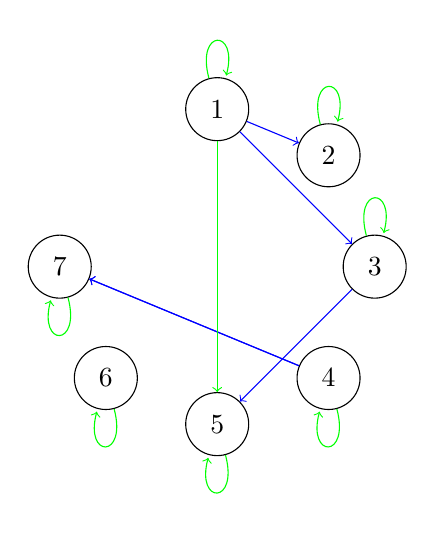
\begin{tikzpicture}[, every node/.style={circle, draw, minimum size=8mm}]
            % Nodes
            \node (1) at (90:2) {1};
            \node (2) at (45:2) {2};
            \node (3) at (0:2) {3};
            \node (4) at (-45:2) {4};
            \node (5) at (-90:2) {5};
            \node (6) at (-135:2) {6};
            \node (7) at (180:2) {7};

            %self loop
            \foreach \i in {1,...,3} {
                \draw[->,green] (\i) edge [loop above] (\i);
            }
            \foreach \i in {4,...,7} {
                \draw[->,green] (\i) edge [loop below] (\i);
            }

            % Edges
            \draw[->,blue] (1) -- (2);
            \draw[->,blue] (1) -- (3);
            \draw[->,blue] (3) -- (5);
            \draw[->,blue] (4) -- (7);
            \draw[->,blue] (4) -- (7);
            \draw[->,green] (1) -- (5);
        \end{tikzpicture}
        \caption{First model}
    \end{minipage}
    \quad
    \begin{minipage}[b]{0.45\linewidth}
        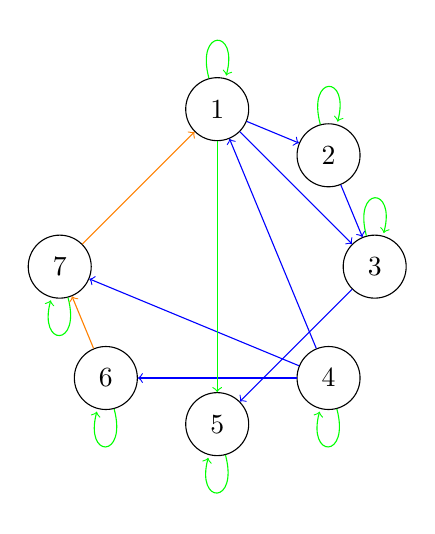
\begin{tikzpicture}[, every node/.style={circle, draw, minimum size=8mm}]
            % Nodes
            \node (1) at (90:2) {1};
            \node (2) at (45:2) {2};
            \node (3) at (0:2) {3};
            \node (4) at (-45:2) {4};
            \node (5) at (-90:2) {5};
            \node (6) at (-135:2) {6};
            \node (7) at (180:2) {7};

            %self loop
            \foreach \i in {1,...,3} {
                \draw[->,green] (\i) edge [loop above] (\i);
            }
            \foreach \i in {4,...,7} {
                \draw[->,green] (\i) edge [loop below] (\i);
            }

            % Edges
            \draw[->,blue] (1) -- (2);
            \draw[->,blue] (1) -- (3);
            \draw[->,blue] (3) -- (5);
            \draw[->,blue] (4) -- (6);
            \draw[->,blue] (4) -- (7);
            \draw[->,blue] (2) -- (3);
            \draw[->,green] (1) -- (5);
            \draw[->, orange] (6) -- (7);
            \draw[->, orange] (7) -- (1);
            \draw[->,blue] (4) -- (1);
        \end{tikzpicture}
        \caption{Second model}
    \end{minipage}
    \end{figure}
    
    The first model expresses $T$ as the reflexive transitive closure of the input $E$, whereas the second model expands the first model and adds more additional atoms to a model.
\end{contexample}

Such an ambiguity is not ideal when we want to compute the query results of datalog. Some fragments of logic programming allow multiple models such as answer-set programming, but for datalog, we want a unique model. This is known as the least model. For this, we need to define what least means and show that it exists.

We call a set of ground atoms an \textit{interpretation}. An interpretation represents all true atoms. We want to define the model property from first-order logic for this definition and show then that there exists a least model according to the subset relation.

Recall from first-order logic that $\forall x. \phi(x)$ holds in a structure $\mathcal{A}$ if any element $a \in \mathcal{A}$ we have that $\phi(a)$ holds. As we do not have any function symbols all elements in the universe are constants, so instead of using the universal quantifier we could just create rules by replacing variables with all possible constants.
Formally, this is defined using \textit{groundings} or \textit{instantions} which are functions that map variables to constants. We can apply a grounding $g$ to an atom by replacing every variable $v$ in the terms by $g(v)$ and apply $g$ to a rule by applying it to the head and every atom in the body. At the end of this, we have replaced every variable by a constant and have gained a ground rule. 
The ground program $ground(P)$ of a program $P$ is the set of all ground rules that are the result of applying some grounding to a rule from $P$

We call a ground rule $r$ \textit{true} in an interpretation $I$ if whenever $Body(r)$ is a subset of $I$, then also $Head(r)$ is in $I$.  We call an interpretation $I$ a \textit{model} of a program $P$ if every rule of $ground(P)$ is true in $I$.

So now we have defined models and can define the least model as well. We still need to show that the least model exists for which the following lemma is helpful.

\begin{fact}\label{fact:ModelIntersection}
Let $M_1, M_2$ be two models of a program $P$. Then also $M_1 \cap M_2$ is a model of $P$.
\end{fact}

Therefore the intersection of all models is a model as well and due to the properties of the intersection it is least according to the subset relation. 

In total, we call \[\bigcap_{\text{$M$ is model of $P$}} M\] the \textit{least model} of $P$ and refer to this characterization as the \textit{model-theoretic semantics} of $P$.

\begin{contexample}
    In this example, the first model is actually the least model and the second model is just some other model.

    Therefore the semantic of this program is whenever $Q()$ is given, the reflexive-transitive closure of $E$. 
    If $Q()$ is not given then it is only the reflexive closure.

    Additionally, we see that the rules for $T$ encode general rules whereas the other rules are more a specific input. We might want to reuse these rules for many different instances of $E$, but so far we also need to write a new program.
\end{contexample}

The example raises questions about the reusability of a program. Additionally, we talked in the introduction about database queries but never talked about databases. 

We consider a \textit{database} as a set of ground atoms similar to an interpretation. What is now the semantics of a program $P$ and a database $d$? We simply add every element of $d$ as a fact to $P$ and reuse the previous semantics. Additionally, we can also move all the specific facts from the program into the database and gain a reusable program.
An alternative model definition for a pair of $P$ and $d$ is therefore: An interpretation $I$ is a model for $P$ and $d$ if every ground atom from $d$ is in $I$ and every rule from $ground(P)$ is true in $I$. \cref{fact:ModelIntersection} holds again and we reuse the definition for the database and program case.

Both views are equivalent. We have shown how we can simulate a database by a program. We can simulate the program case with the program and database case by simply using an empty database.

We have now defined the semantics and shown a connection with databases. But this definition is not exactly ideal. In order to find the semantics of a program we would need to check all interpretations and then intersect them all. This is computationally expensive. Is there a simpler way?

We can define a function that computes the least model in a more direct way. For this, we consider the case where only the program $P$ is present.

Consider an interpretation $I$. We call a ground atom $a$ an \textit{immediate consequence} of $I$ if there exists a ground rule $r$ in $ground(P)$ with the head $a$ and $Body(r) \subseteq I$.

The immediate consequence operator $T_P$ adds all immediate consequences to a model. 

\[T_P(I) = \{ a \mid \text {$a$ is an immediate consequence of $I$}\} \]

A fixed point of a function $f$ is an element $k$ such that $f(k) = k$. The repeated application of $T_P$ starting from $\emptyset$ yields a fixed point that is equal to the model-theoretic semantics of a program $P$. 

\begin{contexample}
    We consider again the program $P$. 

    Due to the fact $E(1,3) \leftarrow$, $E(1,3)$ is an immediate consequence of $\emptyset$. Applying $T_P$ again, we have that $T(1,3)$ is an immediate consequence of $\{E(1,3)\}$ due to the rule $T(?x,?y) \leftarrow E(?x, ?y)$ with the grounding 
    
    \[
    g(v) =
    \begin{cases}
        1 & \text{if } v = ?x \\
        3 & \text{else}
    \end{cases}
    \]

    Applying this to every fact, we gain an interpretation $I$ that contains $T(1,3)$ and $T(3,5)$. Then $T(1,5)$ is an immediate consequence of $I$ due to the rule $T(?x, ?z) \leftarrow T(?x,?y) \and T(?y, ?z)$ and the grounding 

    \[
    g'(v) =
    \begin{cases}
        1 & \text{if } v = ?x \\
        3 & \text{if} v = ?y \\
        5 & \text{else}
    \end{cases}
    \]
\end{contexample}

The least fixed-point of $T_P$ is called the \textit{fixed-point semantics} of $P$ and is the basis for most implementations of datalog reasoners. 

Our goal is to explain why an atom is in the datalog result. The third important semantic of datalog helps here. 

A tree $t$ of ground atoms is a proof tree for a ground atom $a$ in a program $P$ and database $d$ if the following three conditions hold:

\begin{enumerate}
    \item the root of $t$ is $a$
    \item for every node $n$ and its children $l$ in $t$ one of the following two conditions holds: 
    \begin{enumerate}
        \item $n \leftarrow l_1 \land ... l_n$ for $l_1,.., l_n \in l$ is a ground rule from $ground(P)$, or
        \item $n$ is a leaf and $n$ is in the database.
    \end{enumerate}
\end{enumerate}

\begin{figure}
    \centering
    \begin{subfigure}[b]{0.45\linewidth}
    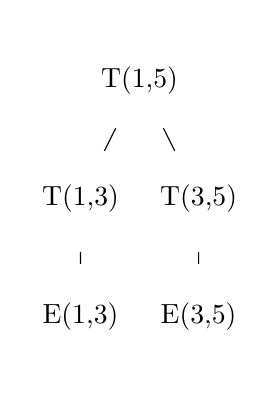
\begin{tikzpicture}[, every node/.style={circle}]
        \node {T(1,5)}
            child {node {T(1,3)}
                child {node {E(1,3)}}
                }
            child {node {T(3,5)}
                child {node {E(3,5)}}};
    \end{tikzpicture}
    \label{prelim:validTree}
    \caption{A valid proof tree}
    \end{subfigure}
    \quad
    \begin{subfigure}[b]{0.45\linewidth}
        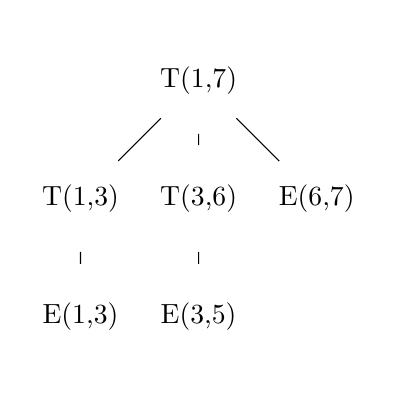
\begin{tikzpicture}[, every node/.style={circle}]
            \node {T(1,7)}
                child {node {T(1,3)}
                    child {node {E(1,3)}}
                    }
                child {node {T(3,6)}
                    child {node {E(3,5)}}}
                child {node {E(6,7)}};
        \end{tikzpicture}
        \caption{An invalid tree}
        \label{prelim:invalidTree}
    \end{subfigure}
    \end{figure}

\begin{contexample}
    The tree in \cref{prelim:validTree} is valid. The leaves of this tree are facts and all other nodes represent ground rules from $ground(P)$ in the previous step.

    The tree in \cref{prelim:invalidTree} is not valid. $E(6,7)$ is neither a fact nor in the database. Additionally there is no rule in $P$ that can result into $T(1,7) \leftarrow T(1,3) \land T(3,6) \land E(6,7)$.
\end{contexample}

The proof-theoretic semantics of a program $P$ and database $d$ is the set of ground atoms that have a valid proof tree. Again this can be shown to be equal to the other semantic definitions. We will formally prove the equality of the proof-theoretic and the model-theoretic semantics of datalog in this work.

In the rules of the program $P$ we note a special rule of the form $T(?x, ?x) \leftarrow$. It is a fact, but not a ground rule and the only rule where this is the case. 
We call a rule $H \leftarrow B_1 \land ... \land B_n$ \textit{safe}, if every variable that occurs in the head also occurs in the body, i.e. \[Vars(H) \subseteq \bigcup_{i \in \{1,..,n\} } Vars(B_i) \]

We call a program safe if every rule in the program is safe. Safe programs are considered better because their result does not depend on the set of constants $C$ which is in practice often either not given or infinite, but only on the specific database and/or the facts in the program.

\begin{contexample}
    We can transform $P$ into the safe program $P'$ by adding a new unary predicate $N$ to the predicate symbols. $P'$ is then the union of $P \setminus \{T(?x, ?x) \leftarrow \}$ and the following rules:
    \begin{equation}
        \begin{split}
            N(?x) &\leftarrow E(?x, ?y) \\
            N(?y) &\leftarrow E(?x, ?y) \\
            T(?x,?x) &\leftarrow N(?x) \\
        \end{split}
    \end{equation}

    The new predicate $N$ (for nodes) represents any elements that occur in the $E$ relation and is used in the body for the reflexive rule.

    If some constants are desired that do not occur in any $E$ relation, one can also directly encode that into the database.
\end{contexample}

What are the semantics of this newly created safe program $P'$? It turns out, that it is equal to the semantics for $P$ for all original predicates, i.e. if we remove all ground atoms that use $N$ we gain the same result. Therefore we state that any program can be transformed into an equivalent safe program.

\subsection{Certifying algorithms}

\begin{figure}
    \centering
    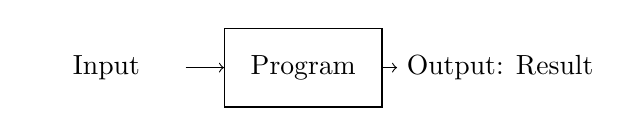
\begin{tikzpicture}[node distance=2.5cm and 20cm, auto]

        \tikzstyle{block} = [rectangle, minimum width=2cm, minimum height=1cm, text centered]
        
        \node [block] (box1) {Input};
        \node [block, right of=box1, draw] (box2) {Program};
        \node [block, right of=box2] (box3) {Output: Result};
        
        \draw [->] (box1.east) -- (box2.west);
        \draw [->] (box2.east) -- (box3.west);
        
    \end{tikzpicture}
    \caption{A convential algorithm}
    \label{fig:programNormal}
\end{figure}

\begin{figure}
    \centering
    \begin{tikzpicture}[node distance=3cm and 3cm, auto]

        \tikzstyle{block} = [rectangle, minimum width=2cm, minimum height=1cm, text centered]
        
        \node [block] (box1) {Input};
        \node [block, right of=box1, draw] (box2) {algorithm};
        \node [block, below of=box3] (box4) {Certificate};
        \node [block, right of=box2] (box3) {Result};
        \node [block, right of=box3, draw ] (box5) {Checker};
        \node [block, right of=box5 ] (box6) {Accept/Not accept};
        \node [block, above of= box6] (box7) {Output};

        \draw [->] (box1.east) -- (box2.west);
        \draw [->] (box2.south) |- (box4.west);
        \draw [->] (box2.east) -- (box3.west);
        \draw [->] (box3.east) -- (box5.west);
        \draw [->] (box4.east) -| (box5.south);
        \draw [->] (box5.east) -- (box6.west); 
        \draw [->] (box3.north) |- (box7.west); 
    \end{tikzpicture}
    \caption{A certifying algorithm algorithm}
    \label{fig:certifyingAlgorithm}
\end{figure}

Most algorithms one encounters either in books like \cite{AlgorithmsBook} or in real programs are comparable to \cref{fig:programNormal}. We have an input, give this into an algorithm which is a black box for us and then we receive a result as an output. Without inspecting the implementation we have to trust that the results are correct.
An alternative to this are \textit{Certifying algorithms} depicted in \cref{fig:certifyingAlgorithm}. They offer an explanation in addition to the result that can be checked independently by the checker or the user themselves. We follow the presentation in \cite{CertAlg} which offers information far beyond this section as well. 

Recall a definition of the class NP from complexity theory:

\begin{definition}[\cite{complexityBook}]
    A language $L \subseteq \{0,1\}^\star$ is in NP if there exists a polynomial $p: \mathbb{N} \to \mathbb{N}$ and a polynomial-time Turing machine $M$ such that forall $x \in \{0,1\}^\star$:

    \[ x \in L  \Leftrightarrow \exists u \in \{0,1\}^{p(|x|)}\text{ s.t. } M(x,u) = 1\]

    If $x \in L$ and $u \in \{0,1\}^{p(|x|)}$ satisfy $M(x,u) = 1$, then we call $u$ a certificate for $x$
\end{definition}

We can generalize this and require an algorithm not only to give us an output $x$ but also a certificate $u$ as a reason why $x$ is the correct output. Then we can either check by ourselves that $x$ is a correct solution according to $u$ or use another program that checks this. As verifying a solution is never harder than computing it, the checker is usually simpler so that we either see directly that the checker is correct or we can formally verify it.

The formal framework of \cite{CertAlg} defines certifying algorithms in the following way. We consider the set $X$ of input values and the set $Y$ of output values of a function $f$. A predicate $\phi: X \to \{true, false\}$ states a precondition for the inputs and another predicate the postcondition $\psi: X \times Y \to \{true, false\}$, $\phi$ allows us the algorithm to only accept part of the input space and $\psi(x,y)$ typically expresses that $y$ is a valid output for the input $x$. In cases where $x$ is not a valid input, we use the new symbol $\bot$ to denote that the algorithm does not return anything and denote by $Y^\bot = Y \cup \{\bot\}$.
The certificate or \textit{witness} from a set $W$ and its correctness is expressed by the predicate $\mathcal{W}: X \times Y^\bot \times W$ with the following properties:

\begin{enumerate}
    \item \textbf{Strong witness property}: Consider a triple $(x,y,w)$ that satisfies the witness predicate $\mathcal{W}$. If $y=\bot$, i.e. the input is not valid, we want $w$ to be a proof of this fact. Else we have that $y\in Y$ and we want $w$ to be a proof that the postcondition is satisfied, i.e.
    \[ \forall x,y,w (y = \bot \land \mathcal{W}(x,y,z) \rightarrow \neg \phi(x)) \land (y \in Y \land \mathcal{W}(x,y,z) \rightarrow \psi(x,y)) \]
    \item \textbf{Simplicity}: This statement above has a simple proof
    \item \textbf{Checkability}: It is possible to check efficiently if $\mathcal{W}(x,y,z)$ holds for a triple $(x,y,z)$
\end{enumerate}

A \textit{(strongly) certifying algorithm} is an algorithm that stops on all inputs $x \in X$ and returns a tuple $\langle y, w\rangle$ such that $\mathcal{W}(x,y,w)$ holds.

This is explained in the following examples. We start with an example from graph theory.

\begin{example}[\cite{CertAlg}]
    Consider the problem of deciding whether a graph $G=(V;E)$ is bipartite, i.e. there exists a partition of $V$ into $V_1, V_2$ with $V = V_1 \cup V_2$ and $V_1 \cap V_2 = \emptyset$, such that for all edges $e \in E$ we have that $e \cap V_1 \neq \emptyset$ and $e \cap V_2 \neq \emptyset$, so that all edges are only between vertices that are in the different partitions.

    The set of inputs $X$ is the set of strings over $\{0,1\}$ and $\phi(x)$ holds whenever $x$ encodes a graph. 
    The postcondition is the following: If $y= true$, then $x$ encodes a bipartite graph. If $y = false$, then $x$ does not encode a bipartite graph.

    Adopting the well-known algorithm for checking whether a bipartite graph, we can construct the following certifying algorithm.

    \begin{enumerate}
        \item Check if $x$ encodes a binary graph. If not return $\bot$ and a witness that describes the problem in the encoding.
        \item Explore the graph in depth-first search and color vertices along the path by alternating colors. If we want to color a vertex by a color $c$ and it already has the color $c'$, we continue exploring another path if $c=c'$, or stop if $c \neq c'$ and return $false$. If that is the case, we have a cycle of odd length in our current path and return this cycle as a witness.
        \item If we reach this step, then all vertices are colored in a way that no neighboring vertices have the same color. Then we return $true$ and the two sets of colored vertices as the witness. 
    \end{enumerate}

    We know from graph theory that a graph is bipartite iff it has no cycle of odd length.

    For any value of $y$ a checker can efficiently check if the returned reason does indeed hold for $x$.
\end{example}

The above example illustrates the example well for a decision problem, but we want to decide whether a set of ground atoms is the semantics of a datalog program and database, i.e. a function problem. The next example illustrates a certifying algorithm for a function problem in number theory.

\begin{example}[\cite{CertAlg}]
    Let $X$ be the set of pairs of natural numbers and $Y$ the set of natural numbers. We want to compute the greatest common divisor, $gcd$, for two numbers $a$ and $b$ that are not equal to zero, i.e. the largest $g \in \mathbb{N}$ that is a divisor of both $a$ and $b$. The precondition $\phi(\langle a, b\rangle)$ is that both $a$ and $b$ are different from zero and $psi(\langle a, b\rangle, g)$ shall me to true, if $g$ is $gcd(a,b)$

    The normal way of computing this involves the Euclidean algorithm, but this is not certifying. The extended Euclidean algorithm however returns in addition to the greatest common divisor $g$ two numbers $s$ and $t$ such that $g = gcd(a,b) = a \dot s + b \dot t$. In \cite{CertAlg}, the back direction is proven, i.e. that if $g$ is a divisor of $a$ and $b$ and $g = a s + b  t$, then $g$ is also the greatest common divisor of $a$ and $b$.

    Therefore a certifying algorithm in order to compute the $gcd$ is the extended euclidean algorithm, that returns as $y$ $gcd(a,b)$ and as the certificate the pair $\langle s, t\rangle$

    A checker then only has to check that $g=a s + b t$ hold and that $g$ divides both $a$ and $b$. 
\end{example}

For decision problems, we require an explanation when the input is in a language as well as an explanation when the input is not in the language. A common misconception is that therefore certifying algorithms are only possible for problems that are known to be in $NP \cap coNP$, which is presumed to not include the interesting $NP$-complete problems. This is not the case as we do not require the certificate to be polynomial in the size of the input. Indeed, SAT-solvers that decide the NP-complete satisfiability problem of propositional logic offer certificates in the DRAT proof format as a model or a proof of unsatisfiability\cite{DRAT}.

In the datalog case, many modern reasoners such as Nemo or Soufflé already offer certificates for atoms in the form of the previously introduced proof trees. We therefore focus on implementing a checker for datalog.

In \cite{CertCheckerWorkflow} an approach to develop checkers for certifying algorithms is outlined. There the checker is implemented in C because already the certifying algorithm itself is written in C++, so that both versions are similar. In order to verify the correctness of the checker they employ the proof assistant Isabelle. The C-code is exported by a tool into Isabelle so that the verification can take place. In Isabelle then the problem is defined and it is proven that the export does fulfill the desired properties. 

In this workflow, we have to trust the correctness of the hardware, the C compiler, the tool that exports C code to Isabelle and of Isabelle itself. Additionally, we have to trust that we have correctly defined and specified the problem in Isabelle.

In this work, we modify this workflow a bit. We use a different proof assistant, Lean, instead of Isabelle. Lean not only a proof assistant but also a functional programming language. Therefore we can implement the checker directly in Lean and do not have to export a model of our code into the proof assistant. Our trust base is therefore smaller, as we no longer need an additional compiler for the language the checker is written in nor a tool to export this into the proof assistant. 


\subsection{Lean}
We introduce in this section Lean, a programming language and proof assistant. As of writing, the current version is Lean 4. A more in-depth introduction can be found in \cite{theoremProvingLean} or \cite{functionalProgrammingLean}.

Lean's core is a small trusted kernel\cite{LeanSysDescr}, that captures the most important functionalities and can be extended by the user. Since version 4 Lean is implemented in Lean itself\cite{Lean4}. The most important libraries for Lean that we will use are the standard library Std4\cite{stdLean} which contains important data structures and tactics and mathlib4\cite{mathlib}, which contains definitions, tactics and theorem from diverse areas of mathematics and computer science.

As we have just heard, Lean can encode many mathematical results. The foundations of mathematics are often built on top of set theory (e.g. \cite{logic}) but most proof assistants instead use \textit{type theory}. Type theory was introduced by Bertrand Russel as an alternative foundation during the foundational crisis of mathematics.

Any element, a \textit{term}, has a \textit{type} in type theory. This is denoted by \lstinline|term:type|. 

\begin{example}
    Different terms in their types are displayed below:
        \begin{lstlisting}
            42:nat
            true:bool
            sort([1,2,3]): List (nat)
            nat: Type
            Type: Type₁
        \end{lstlisting}

        \lstinline|nat| is a natural number, \lstinline|true| is a boolean, the result of the application of \lstinline|sort| to \lstinline|[1,2,3]| has the type \lstinline|List nat|. All previous types have a type as well, \lstinline|Type|. \lstinline|Type| itself also has a type \lstinline|Type₁|. This forms an infinite sequence of \textit{type universes}, that are non-cumulative, i.e. no term has multiple types.
\end{example}


In contrast to set theory, functions are a direct element of type theory and do not need a complicated encoding. For any types \lstinline|A| and \lstinline|B|, there exists the type of functions from A to B, \lstinline| A $\to$ B|.

We can define functions in Lean by the keyword \lstinline|def| similar to other functional programming languages, such as the id function for natural numbers. In the parentheses, we denote an argument \lstinline|x| with its type. Due to currying a function can have multiple arguments. After the colon, we denote the returned type of the function, which is here again a natural number. Therefore we have the following type \lstinline|$\mathbb{N} \to \mathbb{N}$|, as the function takes a natural number as an input and returns a natural number as well. After the \lstinline|:=| we denote the natural number this function returns. 
\begin{lstlisting}
            def id (x: $\mathbb{N}$): $\mathbb{N}$:= x
\end{lstlisting}

Everything we have seen so far holds in general in type theory. Lean itself is based however on a specific type theory, the Calculus of Inductive Constructions (CIC), a dependent type theory\cite{Lean4, CoC}.

The id function we defined above is correct but only works for natural numbers. We would have to implement another id function for booleans, string or any other type. This is rather cumbersome because we never actually use any properties of the specific type. We can generalize this function to help us with this problem.

\begin{lstlisting}
            def id (A: Type)(a: A): A:= a
\end{lstlisting}

This id function has now two arguments. The first argument is the type we want to use it on, the second argument is an element of this type. \lstinline| id $\mathbb{N}$| works as previously and has the type \lstinline|$\mathbb{N} \to \mathbb{N}$|. It seems less clear which type id itself has because this depends on the first argument.
Such types are called \textit{dependent types} and we would denote this specific type as \lstinline|$\Pi$ (A:Type) A $\to$ A|, known as a \textit{Pi type} Intuitively, a Pi type is a function that returns a type for any input value.

In practice, we often do not want to write down too much. We can write the function instead also as:
\begin{lstlisting}
            def id {A: Type}(a: A): A:= a
\end{lstlisting}

Now the type $A$ is an implicit argument, which is denoted by the braces, and Lean can fill it in for the user based on the input $a$. Therefore the user can write just \lstinline|id 42| instead of \lstinline|id $\mathbb{N}$ 42|.

So far we have discussed what types are and how we can define functions that are important for the programming aspect of lean, but this does not tell us much about the use as a proof assistant. Due to the Curry-Howard correspondence a proof of statement can be equivalently seen as a function that has the type of the statement. This type of statements is known in Lean as \lstinline|Prop|. There exist functions like \lstinline|Or: Prop $\to$ Prop $\to$ Prop| and the dependent types form the quantifiers. We view the Pi-type $\Pi (a:A), \beta(a)$ as a function mapping $a$ to the true statements of $\beta(a)$, which is equivalent to the universal quantor. Prop therefore has elements such as \lstinline|$\forall (x:$\mathbb{N}), 0 $\le$ x | or \lstinline| x = y $\lor$ $\neg$ x = y|.

Every statement defines its own type, whose elements are the proofs for it. In contrast to other types, all elements of these types are equivalent which is known as \textit{proof irrelevance}, so that elements of these types only serve as a witness for their truth.

Proofs can be constructed in Lean in two ways.  We start by writing \lstinline|theorem| (or lemma, proposition etc. in mathlib) and denote it as we did for a function. The main difference is that the type is what we want to prove and that the function can not be executed.

\begin{lstlisting}
theorem testTheorem {A: Type}: ∀ (x y z: A), x = y → id y = z → z = x := by
  intro x y z h1 h2
  unfold id at h2
  rw [h1]
  apply Eq.symm
  exact h2
\end{lstlisting}

The proof is done in tactic mode. We open the tactic mode with the keyword \lstinline|by|. At the start our context only contains that $A$ is a type and the goal is $∀ (x y z: A), x = y → id y = z → z = x$, which is compactly written as

\[ \{A:Type\} \vdash ∀ (x y z: A), x = y → id y = z → z = x\]

We apply tactics to change the goal or a hypothesis in the context. These may introduce new goals or fulfill old goals. A proof is finished, when all goals are proven. We explain the proof now in more detail.

\begin{enumerate}
    \item We start with the \lstinline|intro| tactic. This moves elements that are universally quantified or the start of an implication from the goal into the context. Alternatively, one can use \lstinline|revert| to move a hypothesis from the context back to the goal to prove a stronger statement.
    
    At the end, the state is: 

    \[ \{A:Type\} (x y z: A) (h1: x = y) (h2: id y = z)\vdash z = x\]

    \item After that we use the \lstinline|unfold| tactic at the hypothesis h2. This replace \lstinline|id| with its definition in h2, which now looks like this: $(h2: y = z)$
    
    \item We use now the tactic \lstinline|rw|, i.e. rewrite, that replaces in the goal $x$ by $y$ due to the hypothesis $h1$ so that the goal is now $z = y$
    \item The goal is now almost the same as $h2$, but the order is wrong. Therefore we use the apply tactic with
    
    \lstinline|Eq.symm := $\forall \{A:Type\} (a b:A), a = b \rightarrow b = a$ |. 

    Apply tries to match the statements consequent with our goal and opens new goals for the antecedents of this statement.

    Our current proof state is this:

    \[ \{A:Type\} (x y z: A) (h1: x = y) (h2: y = z)\vdash y = z\]

    \item Our goal is now exactly the same as the hypothesis $h2$. The \lstinline|exact| tactic uses $h2$ to complete the goal.
\end{enumerate}

Other important tactics not seen here are \lstinline|by_contra| which allows a proof by contradiction, \lstinline|by_cases| which allows a case distinction or \lstinline|constructor| that splits an and statement into two goals. Lean offers also methods that try to prove goals themselves like \lstinline|simp| that uses lemmas marked with \lstinline|@simp| or \lstinline|tauto|, that can recognize some tautologies. The set of tactics is however not fixed and the user can introduce new tactics to simplify the reasoning process.

The majority of formal proofs in this work are done in tactics mode, but we see above that describing them in natural language is quite verbose. Therefore we will only describe the idea we followed outside of this section.

These proofs are done backwards, i.e. starting from the goal towards the assumptions. There are also forward proofs that start from the assumptions by building hypotheses until we reach the goal or by composing theorems like functions. While this is possible, it was rarely done in this work because. A good source for this is either \cite{theoremProvingLean} or \cite{HitchhikerLogicVer}.

\todo{Tranform the tactic proof into the forward style.}


We can also use \lstinline|def| to define new types. Sets of type \lstinline|A| are in Lean implemented as functions from \lstinline|A| to \lstinline|Prop|. Functions to \lstinline|Prop| are in general not computable so that the membership in a set is also not computable in contrast to for example lists.

\begin{lstlisting}
    def Set (α : Type) := α → Prop
\end{lstlisting}

This introduces a new type. If we want to just use functions that accept contain elements of type \lstinline|Set|, using \lstinline|def| would create a new type for which we would have to define again the set operations $\cup$ or $\cap$. In this case, one can use the \lstinline|abbrev| command which provides a simple alias.

\begin{lstlisting}
    abbrev NatSet := Set $\mathbb{N}$
\end{lstlisting}

The CIC and Lean allow the creation of types by induction. We can create our own implementation of the natural numbers by the \lstinline|inductive| keyword. After that, we list the constructors. These can be constant constructors such as \lstinline|zero| or function creators like \lstinline|succ|
An inductive type may have many constructors of both types or even none as the empty type.

\begin{lstlisting}
    inductive myNat: Type
    | zero: myNat
    | succ: myNat → myNat
\end{lstlisting}

Our definition states that an element of \lstinline|myNat| is either \lstinline|zero| or the result of \lstinline|succ| to some other element of \lstinline|myNat|. Any element of \lstinline|myNat| is only the result of one of these constructors and all elements of \lstinline|myNat| are different.

A typical mathematical definition for this would be: myNat is the smallest set $S$ of elements such that it contains $zero$ and whenever an element $a$ is in $S$, then also $succ(a)$ is in $S$.

We can define for inductive types functions recursively like the add function.

\begin{lstlisting}
    def myNat.add (n m: myNat): myNat :=
    match m with
    | zero => n
    | succ m' => succ (add n m')
\end{lstlisting}

If we want to prove a statement about elements on an inductive type, we can use the \lstinline|induction| tactic to create proofs similar to those by (structural) induction in natural language proofs. If no induction hypothesis is needed one can also use the \lstinline|cases| tactic that creates a goal for every constructor

\begin{lstlisting}
            theorem myNat.add_zero (n: myNat): myNat.add zero n = n := by
                induction n with
                | zero =>
                    unfold add
                    rfl
                | succ n' ih =>
                    unfold add
                    rw [ih]
\end{lstlisting}

We start with the induction tactic to perform an induction over n. Each constructor is listed separately and after the arrow, we start the proof for this constructor. In the zero case, it is enough to unfold the definition of add to get \lstinline|zero=zero| and use \lstinline|rfl| which proves these equalities.

In the succ case, we have two values:  the myNat element $n'$ we use in the constructor of succ and also the induction hypothesis\lstinline|ih: add zero n' = n'|. We can unfold the definition of add again and use \lstinline|rw| to replace \lstinline| add zero n'| by \lstinline|n'| in the goal \lstinline|succ (add zero n') = succ n'|. The \lstinline|rw| tactic applies \lstinline|rfl| at the end automatically to finish the proof.

After defining the natural numbers inductively, we can also define the even numbers by induction. We again have the zero constructor and a succ constructor that now shall represent the next natural number.

\begin{lstlisting}
    inductive evenNat: Type
    | zero: evenNat
    | evenSucc: evenNat → evenNat
\end{lstlisting}

While this works, we see no relation between the elements of myNat and evenNat. We can of course define a function that maps elements of evenNat to myNat and use this to transform any even number to a natural number.

\begin{lstlisting}
    def evenNatToMyNat (e: evenNat) := 
        match e with
        | zero => myNat.zero
        | succ e' => myNat.succ (myNat.succ (evennatToMyNat e'))
\end{lstlisting}

This approach works but is a bit cumbersome. We always need to type this ourselves and if we forget it Lean will complain. There exists however the \lstinline|class Coe|. A class describes an abstract property e.g. of a type and can be implemented by a specific type via \lstinline|instance|.

The \lstinline|Coe| looks (in a simplified version) like this. It takes two types and a function that maps from one type to the other. We can show that this property holds for \lstinline|evenNat| and \lstinline|myNat| by using \lstinline|evenNatToMyNat| to define an instance of this class. Then we can use elements of \lstinline|evenNat| in functions defined for \lstinline|myNat| and Lean will automatically convert them using \lstinline|evenNatToMyNat|.

\begin{lstlisting}
class Coe (α : Type) (β : Type) where
    coe : α → β

instance coeEvenNatMyNat: Coe evenNat myNat := ⟨evenNatToMyNat⟩
\end{lstlisting}

An alternative way of defining types are structures that are comparable to classes in object-oriented languages. Structures have fields that have a type and we start listing them one by one after the \lstinline|where| statement. Structures are like inductive types with a single constructor. Therefore they are not allowed to be recursive, i.e. no structure $A$ may have an element of type $A$, because there would be no base case.
We can build an element of the type of the structure by passing the elements in braces and can use the name of the field to access an element.

\begin{lstlisting}
    structure player where
    (name:String)
    (numGoals: $\mathbb{N}$)
    (active: Bool)

    def player1: player := {
        name := "Test",
        numGoals := 10,
        active := true
    }

    def player1Goals: $\mathbb{N}$ := player1.numGoals
\end{lstlisting}

Returning to our example of myNat, we can define some more functions. In the previous section, we talked about the Euclidean algorithm. We can try to implement it ourselves in Lean. Firstly, we would require the modulo function for that. We will only define it for now to not lose focus and use the keyword \lstinline|sorry| in the value. This closes in proofs any goal or can be used for incomplete functions, but will throw an error if executed.

\begin{lstlisting}
    def myNat.mod (n m: myNat): myNat := sorry
\end{lstlisting}

The Euclidean algorithm can be implemented in the following way:

\begin{lstlisting}
    def myNat.Euclid (a b: myNat): myNat :=
    if b = zero
    then a
    else Euclid b (myNat.mod a b)
\end{lstlisting}

Lean will not accept this function and instead complain in the line of the if that it failed to synthesize an instance of \lstinline|DecidableEq| for myNat. DecidableEq allows us to use $=$ for a type in a function. This is not a trivial requirement as for example the equality of real numbers is undecidable\cite{EqualityRealNumber}. We need to provide a function to Lean that can be used to decide whether two elements of myNat are equal. During the definition of inductive types, we already noted, that all elements of an inductive type are different, which allows us to do this. Luckily, Lean can even do this alone if we tell Lean to do this using the \lstinline|deriving| keyword. It can even derive multiple instances such as the Inhabited instance that states that there exists some default element of this type.

\begin{lstlisting}
    inductive myNat: Type
    | zero: myNat
    | succ: myNat → myNat
    deriving DecidableEq, Inhabited

\end{lstlisting}

Now the error will disappear, but a new one will be introduced. Lean does not recognize the termination of \lstinline|myNat.Euclid|. We have already defined recursive functions before and we did not encounter this problem. In \lstinline|myNat.add| we however used the inductive schema and only did the recursion on $n$ in the case of $succ n$. This allowed Lean to conclude that we only call the function on smaller elements so that the function will terminate.

To show termination, one is required to define some \textit{well-founded relation}, i.e. a relation that does not have any infinite descending chains. Such a relation would be the less-than relation of the natural numbers so it is often convenient to define some size measure that measures the size of our elements in the natural numbers and use this. Such a function exists automatically for any inductive type and is called \lstinline|sizeOf|. We can provide this and are only left to prove that \lstinline|sizeOf (mod a b) < sizeOf b|, which we will leave open here.

\begin{lstlisting}
def myNat.Euclid (a b: myNat): myNat :=
  if b = zero
  then a
  else Euclid b (myNat.mod a b)
termination_by sizeOf b
decreasing_by
  simp_wf
  sorry
\end{lstlisting}

An alternative to this termination proof would be to mark this function using the \lstinline|partial| keyword, which denotes that this function does not always terminate. This is however often not beneficial as we no longer can no longer use the \lstinline|unfold| tactic to gain the definition of this function in a proof.



We want to take a look at another example of an inductive type, that we will often use namely lists. A list (here List' as List is already a standard definition) is either the empty list or the result of combining a list with a new element and we can define a get function

\begin{lstlisting}
    inductive List' (A: Type): Type
    | nil : List' A
    | cons : A → List' A → List' A
    deriving DecidableEq

    def getElement (A: Type) [Inhabited A] (l: List' A): A :=
    match l with
    | nil => Inhabited.default
    | cons hd _ => hd
\end{lstlisting}

We see in this definition a new type of argument. We want to return an element of the list. If the list is empty, this proves to be difficult. In that case, we return the default element that exists because $A$ is an instance of \lstinline|Inhabited|. Such a type-class parameter is given in brackets and Lean will look for the instance when using this function.

This may not always be the desired behaviour and maybe we want to return nothing if the list is empty. In this case, we can use the \lstinline|Option| Type. It has two constructors, one that contains the element and the other symbolizes that there is nothing. Here $\alpha$ has the type \lstinline|Type u| that symbolizes it works for any type universe.

\begin{lstlisting}
    inductive Option (α : Type u) where
    | none : Option α
    | some (val : α) : Option α
\end{lstlisting}

We will also often use the Exception type. This is uses two types and returns one in the error case and the other in the normal case.

\begin{lstlisting}
    inductive Except (ε : Type u) (α : Type v) where
  | error : ε → Except ε α
  | ok    : α → Except ε α
\end{lstlisting}

\begin{figure}
    \centering
    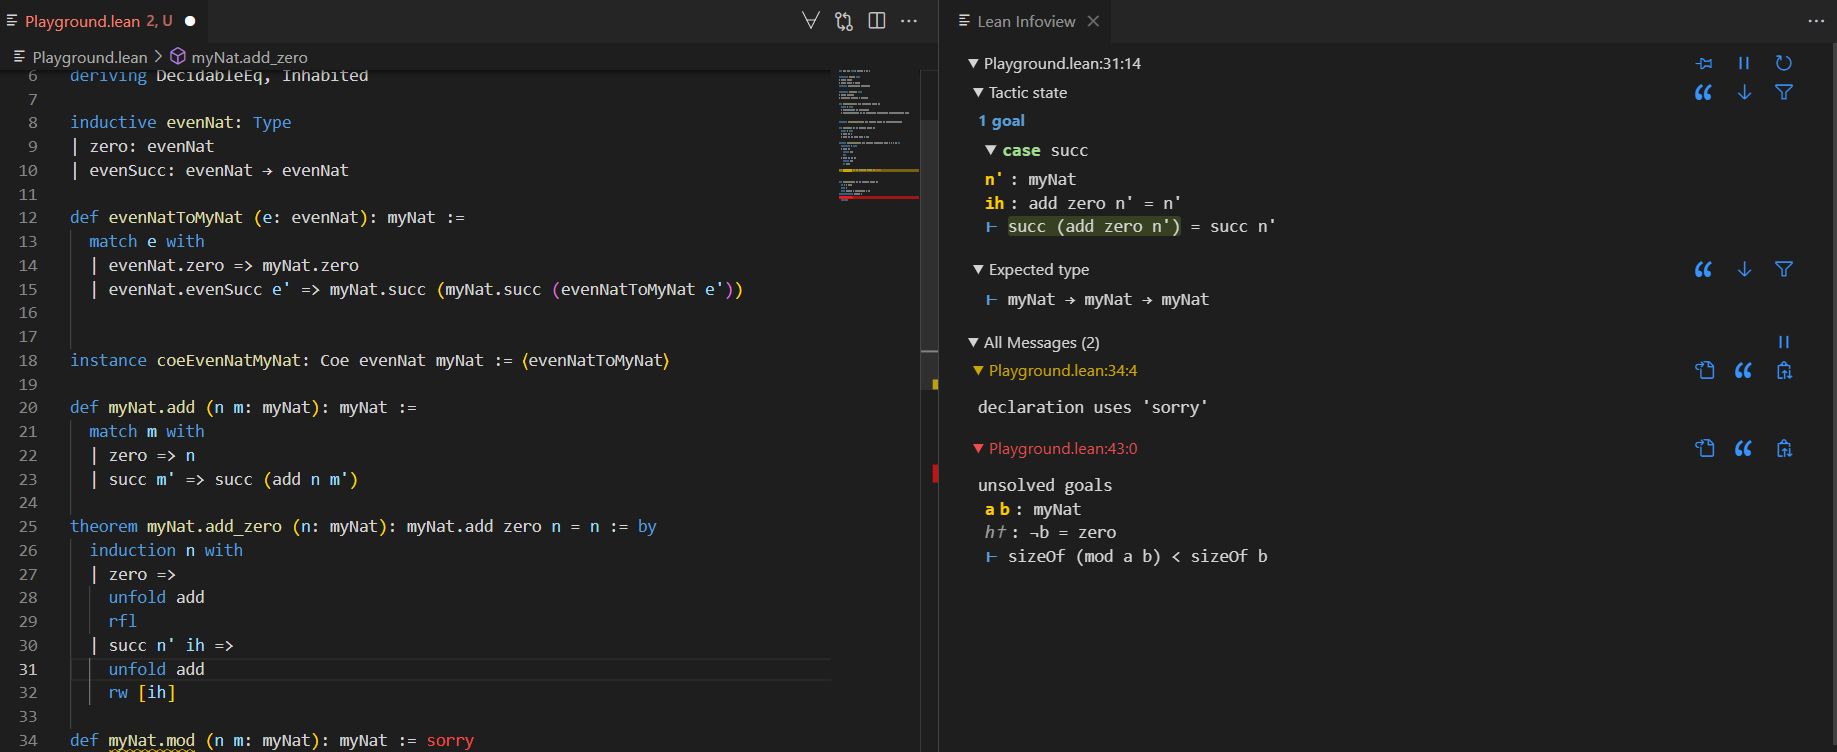
\includegraphics[scale=0.4]{Lean_example.png}
    \caption{An example of Lean in practice. On the left side is the code seen and on the right side the context in a proof with the current goal}
\end{figure}

    
    \section{Formalization of Datalog}
In the previous section we introduced datalog. Our goal is to check whether ground atoms are the result of correct datalog deriviations. In the pursuit of a correctness proof for our algorithms we need to know what correct deriviations are which we solve by formalizing the syntax and semantics of datalog in Lean. As of writing there is to the best of our knowledge no formalization of datalog in Lean yet. 

There does exist a formalization of datalog in Coq\cite{datalogCoq}. The formalization includes the syntax of datalog and the fixed point semantics of datalog with a certified datalog engine. Similarly, we will also formalize the syntax of datalog. After that the paths will diverge as we are interested in the proof-theoretic semantics of datalog to check proof trees. Additionally, we will also formalize the model-theoretic semantics of datalog for completeness arguments and to have extra security that our formalization holds by proving that both semantics are equivalent.

We recall from the preliminaries that an atom is of the form $A(t_1 \dots t_n)$ for sets of predicate symbols, variables and constants $P,V$ and $C$ and an arity function $ar: P \to \mathbb{N}$. If we were to directly formalize this an atom would be defined in the following way, where we use types instead of sets.

\begin{lstlisting}
    def atom (C: Type) (P: Type) (V: Type) (ar: P $\to$ $\mathbb{N}$): Type := sorry
\end{lstlisting}

Such a definition is rather verbose with already four arguments. Anything like the semantics that use atoms will require even more inputs. To have a more compact representation we reuse the definition of a signature that shrinks the number of arguments to just one.  We use types instead of sets as this more natural in type theory. We can consider the type as a set. If we were to use sets we would have to decide already which type these sets should have which seems unclear for now. This allows us to instead define later the types we want to use. 

The formalization showed us that the requirements of countability of the sets $P$, $C$ and $V$ were not required. Any result we wanted to prove holds already in this general case. Therefore we forego of modelling this assumption.

A \signature is then a structure that has a type for constants, variables\footnote{We use vars instead because variable(s) is a keyword in Lean} and predicate symbols and an arity function.

\begin{lstlisting}
structure (.\signature.) where
  (constants: Type)
  (vars: Type)
  (predicateSymbols: Type)
  (predicateArity: predicateSymbols → ℕ)
\end{lstlisting}

In the future unless denoted otherwise we will always use a fixed signature $\tau$ and assume that all types have the \lstinline|DecidableEq| and \lstinline|Hashable| properties to use Lean automatic derivation for later uses in the program. 

Another requirement was that the sets of constants and variables are distinct. This proved again to be unnecessary in our formalization because we define terms as an inductive type with a constructor for each the constant and the variable case. Therefore constants and variables in an atom will always be distinct.

\begin{lstlisting}
    inductive (.\term.) (τ: signature): Type
    | constant : τ.constants → term τ
    | variableDL : τ.vars → term τ
    deriving DecidableEq, Hashable
\end{lstlisting}

For an atom we have fields for the symbol, the list of terms and a proof that the length of the list matches the arity of the symbol.

\begin{lstlisting}
structure (.\atom.) where
  (symbol: τ.predicateSymbols)
  (atom_terms: List (term τ ))
  (term_length: atom_terms.length = τ.predicateArity symbol)
deriving DecidableEq, Hashable
\end{lstlisting}

Two structures of the same type are equal if all their fields are equal. Due to proof irrelevance we gain the following expected criteria for the equality of atoms.

\begin{lemma}[\atomEquality]\label{lem:atomEquality}
    For all $\tau$-atoms $a_1, a_2$, we have $a_1 = a_2$ iff their \lstinline|symbol|s and \lstinline|atom_term|s are equal.
\end{lemma}

Rules and programs can be transformed in straight-forward way. Here we use lists 

\begin{lstlisting}
structure (.\datalogrule.) where
  (head: atom τ)
  (body: List (atom τ))
deriving DecidableEq

abbrev (.\program.) := Finset (rule τ)
\end{lstlisting}

Next, we want to define the ground versions of our previous definitions. Groundings are simply the functions from variables to constants.

\begin{lstlisting}
    def (.\grounding.) (τ: signature):= τ.vars → τ.constants
\end{lstlisting}

We see multiple ways to define ground atoms. Firstly, we can define them like we defined atoms but use constants instead of terms. 

\begin{lstlisting}
structure (.\groundAtom.) (τ: signature) where
  symbol: τ.predicateSymbols
  atom_terms: List (τ.constants)
  term_length: atom_terms.length = τ.predicateArity symbol
deriving DecidableEq, Hashable
\end{lstlisting}

Secondly, we can define ground atoms as a special type atom by constructing a new structure consisting of an atom and a proof that for all terms exists some constant that is equal to it.

\begin{lstlisting}
structure groundAtom (τ: signature) where
    atom: atom τ
    ground: $\forall$ (t: term τ), t $\in$ atom.atom_terms $\rightarrow$ $\exists$ (c: τ.constants), t = term.constant c
\end{lstlisting}

The second variant allows us an easy convertion from ground atoms to atoms by simply returning the atom element. Also we can convert atoms easily to ground atoms as soon as we have the proof. These conversion have to be written by hand in the first variant.

The first variant on the other hand allows us to define functions that create ground atoms more directly. We can take a grounding and just map the term list using this function without having to provide a proof. In the second variant we have to first define the function on the atom level and then have to prove that this operation does not create any variables. This may sound like extra security in case we mess things up, but when defining the terms as a list of constants the type checker of the kernel does the check for us.

The number of conversions is rather limited whereas an easier way to define functions may be useful more often. Therefore we chose the first variant. 

We start by defining these conversions that we now have to do manually. We can convert a ground atom to an atom by mapping every constant to term via \lstinline|term.constant|. The map operation does not change the length of a list of atoms, so that the term length property stays true(\listMapPreservesTermLength).

\begin{lstlisting}
    def (.\groundAtomtoAtom.) (ga: groundAtom τ): atom τ:= {
        symbol:=ga.symbol, 
        atom_terms:= List.map term.constant ga.atom_terms,term_length:= listMapPreservesTermLength ga
    }
\end{lstlisting}

For later proofs it is interesting to know that this is an embedding of the ground atoms into the atoms, i.e. that if two ground atoms are different then the result of their toAtom functions is also different.

For this we need the following result. If two lists are equal than mapping both list by the same function $f$ results in the same list. If the function is injective also the back direction holds, which we prove by induction(\listMapInjectiveEquality).

\begin{lemma}[\groundAtomToAtomEquality]
    Let $a_1, a_2$ be two ground atoms. Then $a_1$ is equal to $a_2$ iff the result of \lstinline|groundAtom.toAtom| of both is equal.
\end{lemma}
\begin{proof}
    If $a_1$ = $a_2$, then also their result is the same.

    For the back direction we know that the results of \lstinline|groundAtom.toAtom| are equal and want to show that they are equal. We use a similar lemma as \cref{lem:atomEquality} for ground atoms(\groundAtomEquality). Therefore we have to show that their symbols and terms are equal. As \lstinline|toAtom| does not change the symbol, the first claim follows. For the second claim we employ the fact the constructors of an inductive type like term.constant are injective functions\footnote{This can be shown with the injection(s) tactic.} and \listMapInjectiveEquality to conclude that the terms are equal.
\end{proof}

We can therefore employ \lstinline|groundAtom.toAtom| safely as the type coercion from ground atom to atom.

For the back direction it would be enough to use a proposition that says that all elements are constants. In later uses such as the definition of safety for rules, it will be beneficial to have a function that computes all variables that occur in an atom. 



After defining the conversions we define ground rules similar to rules.

\begin{lstlisting}
structure (.\groundRule.) (τ: signature) where
  head: groundAtom τ
  body: List (groundAtom τ)
deriving DecidableEq
\end{lstlisting}

We can apply a grounding to a term by replacing a variable by its grounding result and keeping the constant.
\begin{lstlisting}
def (.\applyGroundingTerm.) (g: grounding τ) (t: term τ): term τ :=
  match t with
  | term.constant c => term.constant c
  | term.variableDL v => term.constant (g v)
\end{lstlisting}

Using this function we apply groundings also to atoms and rules. 

\begin{lstlisting}
    def (.\atomGrounding.) (g: grounding τ) (a: atom τ): groundAtom τ := {
    symbol := a.symbol, 
    atom_terms := List.map (applyGroundingTerm'  g) a.atom_terms, 
    term_length := applyGroundingTerm'PreservesLength  g a
    }

    def (.\ruleGrounding.) (r: rule τ) (g:grounding τ): groundRule τ := {
        head:=atomGrounding g r.head, 
        body:= List.map (atomGrounding g) r.body 
    }

\end{lstlisting}

The ground program of a program $P$ is the set of all ground rules that are the result of the application of a grounding to a rule from $P$.

\begin{lstlisting}
    def (.\groundProgram.) (P: program τ) := 
    {r: groundRule τ | ∃ (r': rule τ) (g: grounding τ), r' ∈ P ∧ r = ruleGrounding r' g}
\end{lstlisting}

After finishing the defintion of the syntax, we start formalizing the semantics. We discussed in the preliminaries two ways for the semantics. We decided to formalize the semantics with the database as this is more general. It is simpler to pass an empty database into the checker than writing every fact from the database into the rule file.

In this section we do not want to deviate to much from the path by implementing databases in a complicated way. For now a database is simply something that has a contains function that returns true if an element is in the database. This class can be implemented multiple ways in the algorithm later.

\begin{lstlisting}
class (.\database.) (τ: signature) where
  (contains: groundAtom τ → Bool)
\end{lstlisting}





    \section{Validating proof trees}\label{sec:valTree}

After introducing the problem and modeling datalog in Lean, we now describe the algorithm to verify a solution partially. We focus in this section on the soundness by verifying a given proof tree. In the previous section, we introduced the following characterization for valid proof trees:

\begin{lstlisting}
    def (.\isValid.)(P: program τ) (d: database τ) (t: proofTree τ): 
    Prop :=
    match t with
    | proofTree.node a l => 
    ( ∃(r: rule τ) (g:grounding τ), 
        r ∈ P ∧ 
        ruleGrounding r g = groundRuleFromAtoms a (List.map root l)
        ∧ l.attach.All₂ (fun ⟨x, _h⟩ => isValid P d x)) 
    ∨ (l = [] ∧ d.contains a)
\end{lstlisting}

This is a disjunction so we need procedures to decide for both disjuncts if they are true.
The second disjunct consists of a database check and a check of list emptiness. Both can be done in a straightforward way.

The first part is more interesting. Since we use there existential quantifiers, this is not computable and we have to implement a function for this. While we can simply iterate over the program to check for the existence of a rule $r$, the number of groundings might be exponential or even infinite. Instead of using groundings, we want to use something more sophisticated to check this which we introduce next.


\subsection{Substitutions}
    A grounding is a function from variables to constants. This means we always need to specify for every variable a constant that it is mapped to. This was good in the definitions to ensure that we always get a ground atom, but raises problems in the unification case as the following example demonstrates.

    \begin{example}\label{ex:subsGroun}
        Suppose we want to know whether we can unify the list of terms $l_1 = [?x, ?y]$ with the list of constants $l_2= [a,b]$, i.e. we look for a function $f: V \to C$ such that mapping every element of $l_1$ with $f$ yields $l_2$.

        We start by trying to unify $x$ and $a$. If we use groundings, we might use this function $g = x \mapsto a, y \mapsto a, z \mapsto a$.

        Now we want to use this result and match another term $y$ with the constant $b$. The variable $y$ is already mapped to a different constant, but we cannot say whether this is due to a previous matching process or simply because we needed to define a value for every input.         
    \end{example}
    
    One solution might be to use a special constant symbol that we map variables to that are really unmapped for now.
    Instead, we want to use substitutions that were already introduced in \cite{datalogCoq}. A substitution is a partial mapping from variables to constants. We implement this by mapping to an Option of constant.

    \begin{lstlisting}
    def (.\substitution.) (τ: signature):= τ.vars → Option (τ.constants)
    \end{lstlisting}

    This allows us to only specify what is necessary. We call the substitution that maps any variable to none the empty substitution.
    
    If we apply a substitution to a term and this term is a constant, we do not change the term. If the term is a variable and the substitution does not map the variable to none we replace the variable with the result of the substitution.

    \begin{lstlisting}
    def (.\applySubstitutionTerm.) (s: substitution τ) (t: term τ): term τ :=
    match t with
    | term.constant c => term.constant c
    | term.variableDL v => 
        if p: Option.isSome (s v) 
        then term.constant (Option.get (s v) p) 
        else term.variableDL v
    \end{lstlisting}

    Similar to groundings we can extend this to atoms and rules. 
    
    (\applySubstitutionAtom, \applySubstitutionRule)
    
    As we no longer replace all variables with constants, this only results in atoms instead of ground atoms.

    The main result we want to prove is the following.

    \begin{lstlisting}
    theorem groundingSubstitutionEquivalence 
        (r: groundRule τ) (r': rule τ):
        (∃ (g: grounding τ), ruleGrounding r' g = r) ↔ 
        (∃ (s: substitution τ), applySubstitutionRule s r'= r)
    \end{lstlisting}

    This allows us to replace the grounding check with a substitution check when trying to validate trees and by this, we can bypass the problems that were illustrated in the example above. 

    For the forward direction, we want to find an equivalent substitution for every grounding. We can do this by mapping every variable to the same value of the grounding and place this in the some constructor to obtain an element of the Option type.

    \begin{lstlisting}
    def (.\groundingToSubstitution.) (g: grounding τ): substitution τ
        := fun x => Option.some (g x)
    \end{lstlisting}

    We have to prove that these are equivalent. We defined in the previous section a coercion from ground atoms to atoms. We can also coerce constants to terms by the \lstinline|term.constant| constructor which enables us to use an equality in the following lemma.

    \begin{lemma}[\groundingToSubsitutionEquivTerm]
        Let $t$ be a term and $g$ be a grounding. Then the grounding of $t$ by $g$ is equal to the application of
        
        \lstinline|groundingToSubstitution g| to $t$.
    \end{lemma}
    \begin{proof}
        If $t$ is a constant, then both elements will simply return $t$.

        If $t$ is a variable $v$, then the term grounding by $g$ will return $g(v)$. By the definition of \lstinline|groundingToSubstitution| all variables $v'$ return a some type which contains $g(v')$. Therefore the application replaces $v$ by $g(v)$ and both results are equal. 
    \end{proof}

    Using this result we can extend this equality to the atom level, because in both cases only the terms change by the application of the functions of the previous lemma. Finally, we can extend this to the rule level.
    
    \noindent(\groundingToSubsitutionEquivAtom, \groundingToSubsitutionEquivRule)

    For the back direction, we need an additional property illustrated by the following example.
    \begin{example}
        Consider the program $\mathcal{P} = \{P \leftarrow, Q \leftarrow P\}$ and the signature $C = \emptyset$, $V = \{?x,?y,?z \}$ and $P = \{P,Q\}$

        Any rule in $\mathcal{P}$ is already a ground rule and there exists a substitution, the empty substitution that maps all variables to none, so that the rule is equal to itself as a ground rule.
        
        There is however no grounding that can achieve this. We cannot define a grounding since we have no constant available but have variables that need to be mapped somewhere. Therefore the equivalence does not hold here.
    \end{example}

    For the equivalence to hold we always need at least one constant symbol. There exist at least two possibilities to achieve this in Lean. We could require that the type of constants is inhabited or that it is non-empty. We decided to use the first as the inhabited class offers directly a constant, the default value, whereas the class non-empty only proves that such an element exists and requires the axiom of choice to extract it.

    \begin{lstlisting}
        def (.\substitutionToGrounding.) [ex: Inhabited τ.constants] 
        (s: substitution τ): grounding τ :=
        fun x => 
        if p:Option.isSome (s x) 
        then Option.get (s x) p 
        else ex.default
    \end{lstlisting}

    \begin{contexample}
        If we add the fresh symbol $a$ to $C$, we can use the function $f: V \to C, v \mapsto a$. This will not cause any problems during the verification of a proof tree. While it increases the number of groundings it will not result in any match if used, because it does not occur in the proof tree.
    \end{contexample}

    This is similar to the Herbrand base where we also add a constant symbol if no constant is present.

    For the back direction, we prove again that it is equivalent on terms and then the atom and rule case easily follow. As applying a substitution to a term does not always yield a constant, we require that all variables of the term are mapped to a constant by the substitution. We formalize this requirement using the substitution domain as the set of defined variables of a substitution.

    \begin{lstlisting}
        def (.\substitutiondomain.) (s: substitution τ): Set (τ.vars) := 
            {v | Option.isSome (s v) = true}
    \end{lstlisting}
    
    

    \begin{lemma}[\substitutionToGroundingEquivTerm]
        Let $\tau$ be a signature that contains at least one constant symbol. For any substitution $s$ and term $t$ such that the term variables of $t$ are a subset of the substitution domain of $s$, also grounding $t$ by \substitutionToGrounding of $s$ yields $c$.
    \end{lemma}
    \begin{proof}
        If $t$ is a constant, then it must be equal to $c$ and neither the grounding nor the substitution change the term.

        If $t$ is a variable $v$, then $s(v)$ must be $c$ in order to be equal to $c$. Therefore $s(v)$ is defined and \lstinline|substitutionToGrounding| replaces $v$ by the same value, so that the equality holds as well.
    \end{proof}

    In the end, we obtain the desired theorem with the additional requirement on the set of constants. Note that for the back direction if the application of a substitution to a rule yields a ground rule, then all variables of the rule are in the substitution domain. 
    
    \noindent(\applySubstitutionRuleIsGroundImplVarsSubsetDomain)
    \begin{theorem}[\groundingSubstitutionEquivalence]\label{trm:groundingSubstitutionEquivalence}
        Let $\tau$ be a signature that contains at least one constant symbol. Then for any $\tau$ rule $r'$ and ground rule $r$ we have that there exists a grounding $g$ such that grounding $r'$ by $g$ yields $r$ iff there exists a substitution $s$ such that applying $s$ to $r'$ yields $r$.
    \end{theorem}

    When introducing substitutions, we had the goal to only add what is needed to a substitution and usually, we want the smallest possible substitution. In order to formalize this, we want to define a partial order on substitutions, that is denoted by $\subseteq$.
    
    A substitution $s_1$ is then a subset of a substitution $s_2$, if both substitutions agree on the substitution domain of $s_1$. Outside of this $s_1$ is never defined, whereas $s_2$ might be, so we view $s_1$ as smaller.

    \begin{lstlisting}
    def (.\substitutionsubs.) (s1 s2: substitution τ): Prop :=
    ∀ (v: τ.vars), v ∈ substitution_domain s1 → s1 v = s2 v
    \end{lstlisting}

    This relation is by defintion reflexive (\substitutionsubsrefl). It is also anti-symmetric (\substitutionsubsantisymm). Since $s_1 \subseteq s_2$ anywhere where $s_1$ is defined $s_2$ is defined as well and has the same value. Since $s_2 \subseteq s_1$ anywhere where $s_2$ is defined the same holds, so that they have the same substitution domain and on it the same values. By the principle of function extensionality, both functions are equal.

    Lastly, it is also transitive (\substitutionsubstrans), so it is an instance of a partial order.

\subsection{Unification}

We know that instead of finding a grounding, it suffices to find a substitution. Now we want to describe an algorithm that tells us whether the ground rule that is formed from a vertex of the proof tree and its children is in the ground program. For this, we take inspiration from the unification problem of first-order logic.

In the unification problem of first-order logic we are given a set of equations $s_1 = t_1 \dots s_n = t_n$ between first-order terms and are required to present the most general unifier. A unifier $\mu$ is a function from variables to terms so that if we replace every variable $v$ in $s_i$ and $t_i$ by $\mu (v)$ then all equations are fulfilled. A unifier $\mu$ is called the most general unifier if for every unifier $\sigma$ there exists a function $\tau$ with $\sigma = \tau \circ \mu$.

Our problem is similar and is in general an instance of the following problem.

\begin{definition}
    Let $A$ and $B$ be types and $f: A \to substitution\ \tau \to B$ be a function. We call the following problem an instance of the unification problem.

    \textbf{Input}: A substitution $s$ and elements $a$, $b$ of $A$ and $B$.

    \textbf{Question}: Does there exist a substitution $s'$ with $s \subseteq s'$ and $f(a, s') = b$. If such an $s'$ exists we call it a solution. We call $s'$ a minimal solution if we have $s' \subseteq s^\ast$ for any solution $s^\ast$.
\end{definition}

An example would be to consider $A$ as the type of terms and $B$ as the type of constants. Then $f$ is \lstinline|applySubstitutionTerm|. Another instance would be with atoms and ground atoms. $a$ is in general the normal object and $b$ the ground object.

An algorithm to solve the first-order unification problem is the algorithm of Martelli and Montanari \cite{MartMont} and is depicted below.


\begin{algorithm}
    \caption{Algorithm of Martelli and Montanari}
\begin{algorithmic}
    \While {There exists some equation for which a transformation is possible}
    \State Pick this equation $e$ and do one of the following steps if applicable
    \begin{enumerate}
        \item If $e$ is of the form $t = t$, then delete this equation from the set.
        \item If $e$ is of the form $f(t_1, .., t_n) = f(s_1,.., s_n)$, then delete $e$ and add $n$ new equations of the form $t_i = s_i$
        \item If $e$ is of the form $f(t_1, .., t_n) = g(s_1,.., s_m)$ with $g \neq f$, then stop and reject.
        \item If $e$ is of the form $f(t_1,..,t_n) = x$ for a variable $x$ and delete $e$ and add an equation with the swapped order to the set
        \item If $e$ is of the form $x=t$ for some variable $x$, then check if x occurs in t. If it does, then stop and reject. If not map all $x$ to $t$ in the set.
    \end{enumerate}
    \EndWhile
\end{algorithmic}
\end{algorithm}

This algorithm offers a good starting point for our algorithms, but we know that certain transformations can't occur in the limited syntactic form we operate in. Additionally, we want to output a substitution instead of just answering whether a substitution exists. It is sufficient to do it here, but will later be important. Instead of mapping all $x$ to $t$ as done there in step 5, we will add $x\mapsto t$ to a substitution that is presented as an input. If a variable occurs on the left side, we will check whether it is already in the domain of the substitution and if so check if its current value is consistent with the right side.
Steps 2 and 3 deal with function symbols that are not allowed in our language apart from constants, so that we can replace them by checking whether two constants are equal in the term case. For atoms or rules, we use something similar and split the problem into multiple smaller problems for terms or atoms.

Finally, as the one side of the equation is always a ground object there will never be a variable on this side, so we do not have to swap the equation as in step 4.

We will start by matching a term to a constant with the following algorithm.

\begin{lstlisting}
    def (.\matchTerm.) (t: term τ)(c: τ.constants) (s: substitution τ):
    Option (substitution τ) :=
    match t with
    | term.constant c' =>
        if c = c'
        then Option.some s
        else Option.none
    | term.variableDL v =>
        if p:Option.isSome (s v)
        then  
            if Option.get (s v) p = c
            then
                Option.some s
            else
                Option.none
        else
            extend s v c
\end{lstlisting}

We are given a term $t$, a constant $c$ and a current substitution $s$ and want to return the minimal solution.

This is done by case distinction. If $t$ is a constant, then we either return $s$ if $t$ is equal to $c$ or return none as two different constants can not be unified by a substitution. If $t$ is variable, we check if $t$ is in the domain of $s$. If it is already defined we check if the value matches the required value. If it is not defined we extend $s$ with the new mapping $v \mapsto c$.
Formally extend is defined in the following way:

\begin{lstlisting}
    def (.\extend.) (s: substitution τ) (v: τ.vars) (c: τ.constants) :
        substitution τ 
    := fun x => if x = v then Option.some c else s x
\end{lstlisting}

We now formally prove the correctness of this algorithm. 

\begin{lemma}[\matchTermFindsSolution]
    Let $t$ be a term, $c$ be a constant and $s$ be a substitution. If matchTerm $t$ $c$ $s$ returns a substitution $s'$, then $s'$ is a solution.
\end{lemma}
\begin{proof}
The proof is done via case distinction. Suppose firstly that $t$ is a constant $c'$. Since matchTerm returned a substitution we must have that $c$ and $c'$ are the same constant and therefore $s'$ is $s$. Applying a substitution to a constant does not change it, so $s' t = s' (c') = c' = c$. Additionally since $\subseteq$ is a partial order and $s' = s$, we have that $s \subseteq s'$

Now we assume that $t$ is a variable $v$. Now we do another case distinction on whether $s v$ is defined or not. If it is defined, $v$ must already be mapped to $c$ and we return $s$ as this is a solution as seen previously. If it would be mapped to something else, then matchTerm would return none, which would violate our assumptions.
If it is not defined, we use extend. After that $v$ is mapped to $c$, so that $s' t$ will be equal to $c$. Now we finally have to show that $s \subseteq$ extend $s$ $v$ $c$. We only change the value of $v$. Since $s v$ was not defined earlier, for any variable in the domain of $s$, $s$ and extend $s$ $v$ $c$ agree, so that it is fulfilled(\ssubsetextends).
\end{proof}

We have proven so far that matchTerm returns a solution, but it might not be a minimal solution. As we can transform any grounding into a substitution a match function might return the grounding in \cref{ex:subsGroun}. As we are interested in matching rules and ground rules, we will have to match many terms so that the minimality is an important property for later proofs.

\begin{lemma}[\matchTermFindsMinimalSolution]\label{lem:matchTermMin}
    Let $t$ be a term, $c$ be a constant and $s$ be a substitution. If matchTerm $t$ $c$ $s$ returns a substitution $s'$, then $s'$ is a minimal solution.
\end{lemma}
\begin{proof}
We already know that $s'$ is a solution and only have to show its minimality. Let $s^\ast$ be an arbitrary solution.

We prove the minimality again via case distinction on $t$. If $t$ is constant, then $s'$ must be equal to $s$. Since $s^\ast$ is a solution we have that $s \subseteq s^\ast$ and since $s=s'$, we gain the desired result.

Now we consider the case of $t$ being a variable $v$ and do a case distinction whether $s v$ is defined. If it was already defined, then $s'$ must again be equal to $s$, so that the claim is fulfilled by the argument above.
If $s v$ was not defined, we have to show that extend $s$ $v$ $c$ is a subset of any such $s^\ast$. We assume for a contradiction that this is not the case. Then there must be a variable in the domain of extend $s$ $v$ $c$ such that extend $s$ $v$ $c$ and $s^\ast$ differ. Suppose this variable is $v$. Then $s^\ast$ would either not be defined for $v$ or map $v$ to some other constant $c'$. In both cases $s^\ast v \neq c$, so that $s^\ast$ would not be a solution and we would have reached a contradiction.
If it is some other variable $v'$, then the value of extend $s$ $v$ $c$ is simply the value of $s$. Since $s^\ast$ maps $v$ to a different value compared to $s$, $s$ would not be a subset of $s^\ast$ and we have reached another contradiction.
\end{proof}

So we know that if matchTerm returns a substitution then it is a minimal solution. This holds however already if we never return a solution. We have to prove that if no substitution exists, then there is no solution.

\begin{lemma}[\matchTermNoneImpNoSolution]
    Let $t$ be a term, $c$ be a constant and $s$ be a substitution. If matchTerm $t$ $c$ $s$ returns none, then there exists no solution.
\end{lemma}
\begin{proof}
This is again done via case distinction on the type of $t$. If $t$ is a constant $c'$, then $c'$ must be different from $c$, so that matchTerm returns none. Then no substitution can map $t$ to c.

If $t$ is a variable $v$, then $s v$ must be defined and mapped to a different value compared to $c$. Then again no such $s'$ can exist. If $s$ would be a subset of $s'$, then $s'$ would not unify $t$ with $c$ and if $s'$ would unify $t$ with $c$ then $s$ would not be a subset of $s'$.
\end{proof}

After proving the correctness for terms we now want to move up to atoms. Unfortunately, we cannot use recursion directly on the term list of an atom because an atom requires a proof that the length of the list is equal to the arity of the relation symbol, which fails when we do recursion on the list. Therefore we first establish a new procedure that matches a list of terms with a list of constants, if possible.

\begin{lstlisting}
    def (.\matchTermList.) (s: substitution τ) (l1: List (term τ)) (l2: List (τ.constants)): Option (substitution τ) :=
        match l1 with
        | List.nil =>
            match l2 with
            | List.nil =>
            some s
            | List.cons _ _ =>
            none
        | List.cons hd tl =>
            match l2 with
            | List.nil => none
            | List.cons hd' tl' =>
            let s' := matchTerm hd hd' s
            if p: Option.isSome s'
            then matchTermList (Option.get s' p) tl tl'
            else none
\end{lstlisting}

Here we are given as previously a substitution as an input with the two lists. We see that if both lists differ in length then the function always returns none.
If both lists are the same length we start matching the front and recursively call matchTermList with the resulting substitution until no substitution is found or the entire list is processed.

\begin{lemma}[\matchTermListFindsSolution]
    Let $s$ be a substitution, $l_1$ a list of terms and $l_2$ a list of constants. If matchTermList $s$ $l_1$ $l_2$ returns a substitution $s'$, then $s'$ is a solution.
\end{lemma}
\begin{proof}
    We prove this by induction on $l_1$ for arbitrary $s$ and $l_2$.
    In the base case, $l_1$ is the empty list. Since matchTermList returns something, $l_2$ must also be the empty list. Then $s'$ is equal to $s$. Applying this to an empty list returns an empty list and by reflexivity, we have that $s' \subseteq s$.

    In the induction step we have that $l_1$ is of the form $hd::tl$ and we can similarly assume that $l_2$ is of the form $hd'::tl'$ since matchTermList returns a substitution. Since matchTermList returned a substitution, matchTerm $hd$ $hd'$ also must return a substitution $s^\ast$.

    We then use this as an input to gain $s'$ from matchTermList $s^\ast$ $tl$ $tl'$. By the induction hypothesis, we know that $s^\ast \subseteq s'$ and applying $s'$ to $tl$ results in it being equal to $tl'$. 
    First, we have to show that $s \subseteq s'$. From the correctness proof of matchTerm, we know that $s \subseteq s^\ast$ and from the induction hypothesis we know that $s^\ast \subseteq s'$. Since $\subseteq$ is transitive, the result follows.

    Secondly, we prove that $s'$ is a solution for $hd::tl$ and $hd'::tl'$. From the induction hypothesis, we know that mapping $tl$ with $s'$ yields $tl'$. We know that $s^\ast$ was a solution for $hd$ and $hd'$ and since $s^\ast \subseteq s'$, $s'$ agrees on the domain of $s^\ast$ with $s^\ast$. Therefore it is still a solution for $hd$ and $hd'$. If $hd$ was a constant, then any substitution would do. If $hd$ was a variable, then it is mapped to the same element as by $s^\ast$ so that applying $s'$ to $hd$ yields $hd'$ as well, so that applying $s'$ to $hd::tl$ yields $hd':tl'$. 
\end{proof}

After proving that it is a solution, we prove that the solution is minimal.

\begin{lemma}[\matchTermListFindsMinimalSolution]
    Let $s$ be a substitution, $l_1$ a list of terms and $l_2$ a list of constants. If matchTermList $s$ $l_1$ $l_2$ returns a substitution $s'$, then $s'$ is a minimal solution.
\end{lemma}
\begin{proof}
    We prove this again via induction on $l_1$ for arbitrary $l_2$ and $s$. If $l_1$ is empty then $l_2$ is empty as well and we return $s$. The claim is true by reflexivity.

    In the induction step we have that $l_1$ has the form $hd::tl$ and we can assume that $l_2$ has the form $hd'::tl'$ because a substitution was returned. Let $s'$ be the result of $matchTermList\ l_1\ l_2\ s$. We have to show that for any solution $s^\ast$ for $l_1$, $l_2$ and $s$, we have that $s' \subseteq s^\ast$.
    Let $s^\ast$ be a solution for $l_1$, $l_2$ and $s$. Then it also must be a solution for $hd$, $hd'$ and $s$ and due to \cref{lem:matchTermMin} we have that $matchTerm\ hd\ hd'\ s\ \subseteq s^\ast$. 

    We additionally know that $s^\ast$ is a solution for $tl$, $tl'$ and $s$. Since \matchTerm returns a minimal solution, we also know that it is a solution for $tl$, $tl'$ and $matchTerm\ hd\ hd'\ s$. 

    The result of $matchTermList\ tl\ tl'\ (matchTerm\ hd\ hd'\ s)$ is $s'$. The induction hypothesis tells us that $s'$ is the minimal solution for these input values. Therefore we know that $s' \subseteq s^\ast$ and the claim is proven. 
    
\end{proof}

Finally, the negative case that confirms that the return value of none does indeed state that there is no solution.

\begin{lemma}[\matchTermListNoneImplNoSolution]
    Let $s$ be a substitution, $l_1$ a list of terms and $l_2$ a list of constants. If matchTermList $s$ $l_1$ $l_2$ returns none, then there exists no solution $s'$.
\end{lemma}
\begin{proof}
    We prove this again via induction on $l_1$ for arbitrary $l_2$ and $s$. If $l_1$ is the empty list then $l_2$ must be non-empty and then no solution exists.

    In the induction step we have that $l_1$ has the form $hd::tl$. If $l_1$ is empty, the claim is proven, so we assume that $l_2$ has the form $hd'::tl'$. There are two cases where matchTermList can return none. The first case is when matchTerm $hd$ $hd'$ $s$ returns none. If that is the case there is no $s'$ with $s\subseteq s'$ and applying $s$ to $hd$ will make it equal to $hd'$. Therefore the two lists cannot be equal either and the proof is finished.

    If matchTerm $hd$ $hd'$ $s$ returns a substitution $s^\ast$, then matchTermList $s^\ast$ $tl$ $tl'$ must return none. From the induction hypothesis, we know that there is no substitution $s'$ with $s^\ast \subseteq s'$ and applying $s'$ to $tl$ bringing it equal to $tl'$. Since $s^\ast$ is already the minimal solution to match $hd$ with $hd'$ there cannot exist a solution whose application will lead to $hd$ and $hd'$ being equal and $tl$ and $tl'$ being equal.
\end{proof}

This can be used to create a matchAtom procedure. We are given an atom and a ground atom and check if the symbols are equal. If they are, we use matchTermList to find a unifier.
If the symbols are different, we will never unify them and can already return none.

\begin{lstlisting}
    def (.\matchAtom.) (s: substitution τ) (a: atom τ) (ga: groundAtom τ):
    Option (substitution τ) :=
        if a.symbol = ga.symbol
        then
            matchTermList s a.atom_terms ga.atom_terms
        else none
\end{lstlisting}

The correctness proofs follow from the proofs of matchTermList.

Now we can create a \matchAtomList function similar to \matchTermList and use this to define a \matchRule function. We first try to match the head of the rule with the head of the ground rule. If this returns a solution, we use this as the start for matching the bodies. If not, we will not find a solution and return none.

\begin{lstlisting}
    def (.\matchRule.) (r: rule τ) (gr: groundRule τ):
        Option (substitution τ):=
        let s := matchAtom emptySubstitution r.head gr.head
        if p: Option.isSome s
        then matchAtomList (Option.get s p) r.body gr.body
        else none

\end{lstlisting}

We now prove again that if this returns a substitution then this is a solution and if none is returned then there is no solution using our previous results. 
We want a statement with the quantifier to combine it with the theorem about the equivalence between groundings and substitutions. We can prove this statement by using the result of \matchRule as a witness for the quantifier. For the back direction, we see that this statement implies that a solution exists, which we always find with \matchRule.

\begin{theorem}[\matchRuleIsSomeIffSolution]\label{trm:matchRule}
Let $r$  be a rule and $gr$ be a ground rule. Then there exists a substitution $s$ such that applying $s$ to $r$ yields $gr$ iff \matchRule returns some substitution.
\end{theorem}


We now have a method to replace this quantifier with a computable function and can finally devise the check for tree validation.

\subsection{Tree validation}

We have so far introduced substitutions and have shown a way to decide whether a substitution exists that maps a rule to a ground rule. Now we want to finally show a way to validate trees. As the first step, we want to find whether a ground rule $gr$ we gain from the tree is in the ground program, i.e. that there exists a grounding $g$ (or by \cref{trm:groundingSubstitutionEquivalence} a substitution $s$) and a rule $r$ from the program $P$ so that applying $g$ to $r$ yields $gr$. We want to use the \matchRule function defined earlier for this. 
We can simply pass each rule of the program given as a list of rules into this function and stop when \matchRule returns a some object. This works but requires in the worst case to match every rule in the program with a given ground rule. Suppose that the predicate symbol of the head of the given ground rule is $T$. We can safely discard any rule whose head is not an atom with the predicate symbol $T$. This can be generalized into the symbol sequence which is a list of predicate symbols that starts with the predicate symbol of the head and then the predicate symbols of the body atoms in the order the atoms occur in the body.

\begin{lstlisting}
    def (.\symbolSequence.) (r: rule τ): List τ.predicateSymbols := 
        r.head.symbol::(List.map atom.symbol r.body)

\end{lstlisting}

The equality of symbol sequences is a necessary condition for the existence of substitution that matches a rule with a ground rule, as the application of any substitution does not change the symbols and therefore not the symbol sequence. (\symbolSequenceNotEq).

Now we could iterate over the whole program and calculate the symbol sequence for every rule and only start the matchRule process for those whose symbol sequences are equal to the given ground rule. In the worst case, we still have to iterate over the whole program. It would be even better to preprocess the program into a look-up structure that returns a list of rules for a given symbol sequence.

We use a function of the type \lstinline|List τ.predicateSymbols → List (rule τ)| as the look-up structure and build it iteratively by adding the first rule of the given program to the right symbol sequence element.

\begin{lstlisting}
    def (.\parseProgramToSymbolSequenceMap.) (P: List (rule τ)) 
    (m: List τ.relationSymbols → List (rule τ)): 
    List τ.relationSymbols → List (rule τ) :=
    match P with
    | [] => m
    | hd::tl =>
        let seq:= symbolSequence hd
        parseProgramToSymbolSequenceMap tl 
            (fun x => if x = seq then hd::(m x) else m x)
\end{lstlisting}

If we start this with a function that maps any symbol sequence to the empty list and gain a function $m'$ then for any list of predicate symbols $l$, $m'(l)$ returns exactly those rules in $P$ whose symbol sequence matches $l$. This follows from the following lemma.

\begin{lemma}[\parseProgramToSymbolSequenceMapmem]\label{lem:parseProgramToSymbolSequenceMap}
    Let $P$ be a program and $m$ be a function that maps a list of predicate symbols to the list of rules. Let $m'$ be the result of \lstinline|parseProgramToSymbolSequenceMap P m|. Then for any list of predicate symbols $l$ and rule $r$, we have $r$ is in $m'(l)$ iff $r$ was in $m(l)$ or $r$ is in $P$ and the symbol sequence of $r$ equals $l$.
\end{lemma}
\begin{proof}
    We prove this by induction on the structure of $P$ for arbitrary $m$.

    If $P$ is empty, then $m' = m$ and no rule is a member of $P$ so that the claim follows.

    If $P$ has the structure $hd::tl$, then $m'$ is the result of 

    \begin{lstlisting}
        parseProgramToSymbolSequenceMap tl (fun x => if x = (symbolSequence hd) then hd::(m x) else m x)
    \end{lstlisting}

    Applying the induction hypothesis we see that for any rule $r$ and list $l$, $r$ is in $m'(l)$ iff it is in $tl$ and has the symbol sequence $l$ or was in \lstinline|(fun x => if x = (symbolSequence hd) then hd::(m x) else m x)|

    The only element of $P$ not yet considered was $hd$ and is is either obtained by its symbol sequence or was already there in $m$ so that the proof follows.
\end{proof}

Since at the start $m(l)$ has no member for any $l$, the desired property holds. Now we can use this to check whether a substitution exists. \lstinline|List.any| checks whether any element in $m(symbolSequence gr.toRule)$ matches the ground rule. If that is the case, we simply return unit as a matching rule in $P$ was found. If that is not the case, we return an error message. The Except type allows us to combine these two return types.

\begin{lstlisting}
def (.\checkRuleMatch.) (m: List τ.predicateSymbols → List (rule τ)) (gr: groundRule τ): Except String Unit :=
  if List.any (m (symbolSequence gr.toRule)) 
    (fun x => Option.isSome (matchRule x gr)) = true
  then Except.ok ()
  else Except.error ("No match for " ++ ToString.toString gr)
\end{lstlisting}

\begin{lemma}[\checkRuleMatchOkIffExistsRuleForGroundRule]
    Let P be a program, $m$ be the result of \lstinline|parseProgramToSymbolSequenceMap P (fun _  => [])| and $gr$ a ground rule. Then \lstinline|checkRuleMatch m gr| returns ok iff there exists a rule $r$ in $P$ and a grounding $g$ such that grounding $r$ with $g$ yields $gr$.
\end{lemma}
\begin{proof}
    Let $l$ be the symbol sequence of $gr$. If checkRuleMatch returns ok, then there exists a rule $r$ in $m(l)$ there exists a grounding $g$ such that grounding $r$ by $g$ yields $gr$. By \cref{lem:parseProgramToSymbolSequenceMap} this rule $r$ is a member of $P$ so the claim is proven.

    If checkRuleMatch returns an error, then we have to show that for rule $r \in P$ and grounding $g$ grounding $r$ by $g$ yields a different ground rule compared to $gr$. If $r$ has the same symbol sequence as $gr$, then it occurred in $m(l)$ and since checkRuleMatch returned an error matchRule r gr must return none so that the property holds.

    If $r$ has a different symbol sequence to $gr$ then this property holds as well due to \symbolSequenceNotEq and \cref{trm:groundingSubstitutionEquivalence}.
\end{proof}

This function is almost enough to complete the rule case. We just need to also verify all subtrees. For this we introduce the \lstinline|List.map_except_unit| function that applies a function of the type \lstinline|A → Except B Unit| to a list $l$ until the first error occurs. If no error occurs, then we return Unit which is a type that has only one element $()$ and is the placeholder because we have to return something.

\begin{lstlisting}
    def (.\Listmapexceptunit.) {A B: Type} (l: List A) 
    (f: A → Except B Unit): Except B Unit :=
    match l with
    | [] => Except.ok ()
    | hd::tl =>
        match f hd with
        | Except.ok () => List.map_except_unit tl f
        | Except.error b => Except.error b
\end{lstlisting}

We can prove by induction that this function returns unit iff $f$ returns unit on all elements of the list $l$ (\ListmapexceptunitIsUnitIffAll).

Now we have the necessary tools to check whether a given proof tree is valid which is done by the \treeValidator. For a tree with the root $a$ and subtrees $l$, we do a case distinction whether $l$ is empty. If $a$ is additionally an element of the database, then we accept $a$ because we are in the database case. If not we use checkRuleMatch to check for the rule case. If this returns ok, then we can already accept $a$ because there are no subtrees.

If not we can only be in the rule case and first use checkRuleMatch and if this returns ok, then we check all subtrees using the treeValidator again called via \Listmapexceptunit.

\begin{lstlisting}
def treeValidator (m: List τ.predicateSymbols → List (rule τ)) (d: database τ) (t: proofTree τ) : Except String Unit :=
  match t with
  | tree.node a l =>
    if l.isEmpty
    then  if d.contains a
          then Except.ok ()
          else
            match checkRuleMatch m {head:= a, body := List.map root l} with
            | Except.ok _ => Except.ok ()
            | Except.error msg => Except.error msg
    else
      match checkRuleMatch m {head:= a, body := List.map root l} with
      | Except.ok _ => List.map_except_unit l.attach (fun ⟨x, _h⟩ => treeValidator m d x)
      | Except.error msg => Except.error msg
\end{lstlisting}

Using the previous lemmas and induction over the height of the tree for the recursive calls, we prove the correctness of the treeValidator.

\begin{theorem}[\treeValidatorOkIffIsValid]\label{trm:treeValidator}
    Let P be a program, $m$ be the result of \lstinline|parseProgramToSymbolSequenceMap P (fun _  => [])| and $d$ be a database. For any proof tree $t$, \lstinline|treeValidator m d t| returns ok iff $t$ is valid for $P$ and $d$.
\end{theorem}


If we want to validate the whole result of a datalog program, we will often need many proof trees and a function that can validate them. Additionally, we need to preprocess the program to gain the map from symbol sequences to rules. We can reuse the \Listmapexceptunit function for this purpose

\begin{lstlisting}
def (.\validateTreeList.) (P: List (rule τ)) (d: database τ) (l: List (proofTree τ)) : Except String Unit :=
let m:= parseProgramToSymbolSequenceMap P (fun _ => [])
List.map_except_unit l (fun t => treeValidator m d t)
\end{lstlisting}

Using \cref{trm:treeValidator} and \ListmapexceptunitIsUnitIffAll, we can show that this function returns ok iff all trees in $l$ are valid. We know that a ground atom $ga$ is in the proof-theoretic semantics if there exists a proof tree with the root $ga$ so that we can conclude the set of roots of the trees in $l$ is a subset of the semantics. 


It turns out however that we can do a bit better and prove a stronger statement as the following example shows.
\begin{example}
    Consider the program $P:$
    \begin{align*}
        & A(?x, ?z) \leftarrow B(?u,?x, ?y, ?z). \\
        & B(?u,?x, ?y, ?z) \leftarrow C(?u,?x), D(?z, ?y). \\
        & C(a,b). \\
        & D(c,d).
        \end{align*}

    The result of this program over an empty database is \[\{A(a,c), B(a,b,d,c), C(a,b), D(c,d)\}\] and a proof tree is depicted below for each of them.


    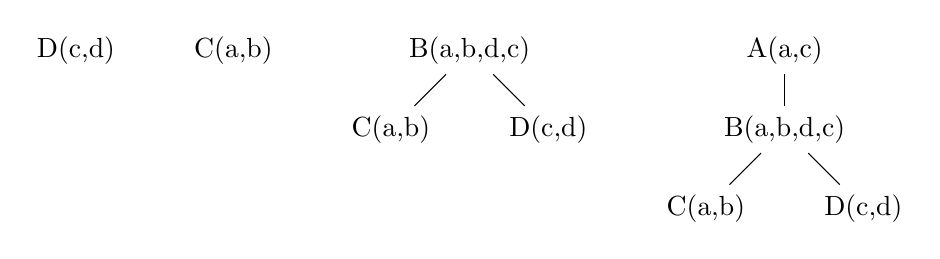
\begin{tikzpicture}
        \node (D1) at (0,0) {D(c,d)};

        \node (C1) at (2,0) {C(a,b)};

        \node (B1) at (5,0) {B(a,b,d,c)};
        \node (B2) at (4, -1) {C(a,b)};
        \node (B3) at (6, -1) {D(c,d)};
        \draw (B1) -- (B2);
        \draw (B1) -- (B3);

        \node (A1) at (9,0) {A(a,c)};
        \node (A2) at (9,-1) {B(a,b,d,c)};
        \node (A3) at (8, -2) {C(a,b)};
        \node (A4) at (10, -2) {D(c,d)};
        \draw (A1) -- (A2);
        \draw (A2) -- (A3);
        \draw (A2) -- (A4);
    \end{tikzpicture}

    The proof tree for $A(b,d)$ already contains proofs for all the other elements of the program so it would be enough to check this single tree.
\end{example}

If we want to check a complete datalog result, we therefore do not have to include a proof tree for every element as they can occur in other proof trees already. We formalize this using the element member function that is true if this element is the root or a member in a subtree.

\begin{lstlisting}
def (.\elementMember.) (a: A) (t: tree A): Bool  :=
    match t with
    | tree.node a' l => (a=a') ∨
        List.any l.attach (fun ⟨x, _h⟩ => elementMember a x)
\end{lstlisting}

A tree is valid if all subtrees are valid. In the rule case, we explicitly required this, whereas there are no subtrees in the database case. Any element member is the root of some subtree and therefore any element member of a valid proof tree is in the proof-theoretic semantics 

(\allTreeElementsOfValidTreeInSemantics).

This allows us to establish the alternative property of validateTreeList. We added the requirement of all proofs being valid to prove the back direction. As the validity of a proof tree is in general not preserved under permutation, it is not sufficient to just require every element member to be in the proof-theoretic semantics.

\begin{lemma}[\validateTreeListUnitIffSubsetSemanticsAndAllValid]
    Let $P$ be a program, $d$ be a database and $l$ a list of proof trees. Then validateTreeList returns ok iff all element members of the trees in $l$ are in the proof-theoretic semantics and all trees in $l$ are valid.
\end{lemma}
\begin{proof}
    For the forward direction, we already noted that if validateTreeList returns ok, then every tree in $l$ must be valid. By the previous lemma therefore any element member of one of these trees is in the proof-theoretic semantics.

    For the back-direction follows from the previous observation, that validateTreeList returns ok iff all trees in $l$ are valid.
\end{proof}

Now it is enough to pass just the proof tree for $A(a,c)$ from our example into the checker to validate the whole input and use in general fewer trees. 

    
    \section{Validating graphs}

We have finished the last section with a method to check whether a result is a subset of the semantics. For this we need a list of trees representing the result set. Finding such a list is however difficult. Viewing a tree as a set of its elements we see that it is an instance of the NP-hard set cover problem. Additionally, we found in practice that the datalog reasoner we used did only return a list of derivations. Constructing trees from this turned out to be computationally expensive, but the output can be interpreted as a directly acyclic graph. In the following section we describe how to validate such a graph.

A number of different results of graph theory are already proven in mathlib. Nonetheless, we defined our own graph model in Lean for this section due to two main reasons. Firstly, the graph defined in mathlib is a undirected graph, but we require a directed graph so that we can see for a vertex (which represents a ground atom) which neighbors were used to derive it and which neighbors were derived from it. Secondly, the graph represents the edge relation as a map to \texttt{Prop} which is in general not computable.


Our graph model consists of a list of vertices and a function that maps to each element the list of its predecessors. Representing the vertices as a list allows us to iterate over all vertices when validating the graph. We used a function to the predecessors instead of a adjancency matrix similar to the definition in mathlib in order to directly get the predecessors to a node instead of having the iterate over all vertices and check the adjancency matrix. This approach does have a small drawback. Suppose we want to determine whether a property holds for every vertex and do this by exploring the graph using depth-first search and we find a counterexample by following the predecessors. Nothing states that this vertex is actually in the graph, i.e. the list of vertices. This is an undesireable property so that we additionally ask for a proof that the predecessors of every vertex are again vertices in the graph.

\begin{lstlisting}
    structure Graph (A: Type) where
        (vertices: List A)
        (predecessors: A → List A)
        (complete: ∀ (a:A), a ∈ vertices →  
        ∀ (a':A), a' ∈ predecessors a → a' ∈ vertices)
\end{lstlisting}

A standard definition of graph theory are walks as a sequence of connected edges. As we do not have edges directly, we represent this as a list of elements with two properties. A list of elements is a walk in a graph, if all elements are a vertices of the graphs and neighboring vertices are connected via the the predecessor relation of the graph. Due to the completeness property of the graph it would also be sufficient to express that the last element of the path is in the graph. 

\begin{lstlisting}
    def isWalk (l: List A) (G: Graph A): Prop :=
    ( ∀ (a:A), a ∈ l → a ∈ G.vertices ) 
    ∧ ∀ (i: ℕ), i > 0 → ∀ (g: i < l.length), 
    l.get (Fin.mk i.pred (pred_lt i l.length g)) ∈ 
        G.predecessors (l.get (Fin.mk i g) )
\end{lstlisting}

We note that we do allow empty paths. This simplifies some proofs and algorithms even if there is no direct equivalent in graph theory. We specifically use lists as we are going to expand walks at the front when exploring the graph.  

\begin{lemma}
    Let $w$ be a walk in a graph $G$ of the form $a::tl$. Then also $b::a::tl$ is a walk in $G$ for every predecessor $b$ of $a$.
\end{lemma}

Using walks we can define cycles. Every cycle is a walk. Additionally we require that it the start and the end of the walk are equal. In order to have a start and end we have to exclude the empty walks. Additionally, we exclude walks of a single element. Allowing them as cycles would mean that there are no acyclic graphs.

\begin{lstlisting}
    def isCycle (l: List A) (G: Graph A): Prop :=
    if h: l.length < 2
    then False
    else
        have l_not_zero: 0 < l.length :=
        by
        cases ll: l.length with
        | zero =>
            rw [ll] at h
            simp at h
        | succ n =>
            simp

        isWalk l G ∧
            l.get (Fin.mk 0 l_not_zero) 
            = l.get (Fin.mk l.length.pred (Nat.pred_lt (Ne.symm (Nat.ne_of_lt l_not_zero))))
\end{lstlisting}

A graph is then acyclic if no list represents a cycle in it.

\begin{lstlisting}
    def isAcyclic (G: Graph A) := ∀ (l: List A), ¬ isCycle l G
\end{lstlisting}

We need to check whether a given graph is acyclic as only those graphs represent valid derivations. A cycle would mean that we used an atom to derivate itself and we could not get a valid proof tree for this element. We are going to use depth-first search to check whether a graph is acyclic. For this we need an alternative characterization of acyclicity.
A first candidate for this would be the membership in a cycle.

\begin{lemma}
    A graph is acyclic iff no vertice is a member in a cycle.
\end{lemma}

Ideally, we want this characterization to be an iff connection between a vertice and its predecessors. Unfortunately the statement does not hold for this characterization.

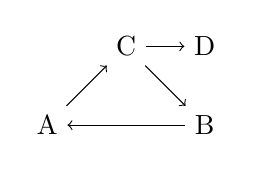
\begin{tikzpicture}
    \node (A) at (0,0) {A};
    \node (B) at (2,0) {B};
    \node (C) at (1,1) {C};
    \node (D) at (2,1) {D};

    \draw[->] (B) -- (A);
    \draw[->] (C) -- (B);
    \draw[->] (A) -- (C);
    \draw[->] (C) -- (D);
\end{tikzpicture}

D is not a member in a cycle, but its predecessor C is, so that an iff does not hold. Instead we see that D can be reached from a cycle using some walk. If it can be reached from a cycle, then also one of its predecessors can be reached from a cycle. We are going to formalize this idea in the following lemmas.

Let $a$ and $b$ be two nodes. We say that $a$ can reach $b$ in $G$ if there exists a walk in $G$ that starts with $a$ and ends with $b$.

\begin{lstlisting}
    def canReach (a b: A) (G: Graph A):= ∃ (w: List A) (neq: w ≠ []),
    isWalk w G ∧
    w.get (Fin.mk 0 (getFirstForNonequal_isLt w neq)) = a ∧
    w.get (Fin.mk w.length.pred (getLastForNonequal_isLt w neq)) = b
\end{lstlisting}

A singleton path allows us to show that any element can reach it self. Additionally, if $a$ can reach $b$ and $b$ is a predecessor of $c$ we can extend the path from $a$ to $b$ with $c$ in order to demonstrate that $a$ can reach $c$. Using the \texttt{canReach} predicate we can now express a different characterization for acyclicity, being reachable from a cycle. A node $a$ is reachable from a cycle $c$, if there exists a node $b$ in the cycle that reaches $a$. In the previous example $D$ is reached from a cycle as $C$ is in a cycle and $C$ reaches $D$. The same holds for $C$ as $C$ reaches itself.

\begin{lstlisting}
    def reachedFromCycle (a:A) (G: Graph A):=
        ∃ (c: List A), isCycle c G ∧ ∃ (b: A), b ∈ c ∧ canReach b a G
\end{lstlisting}

\begin{lemma}
    A graph $G$ is acyclic iff all vertices of $G$ are not reached from a cycle.
\end{lemma}
\begin{proof}
    If $G$ is acyclic, then showing that all vertices of $G$ are not reached from a cycle is equivalent to showing that any cycle in $G$ cannot reach any element. Due to the acyclicity we know that no cycles exist in G so that the first direction is shown.

    The back direction is proved via contradiction. Assuming that the graph is not acyclic, we know that there must exist a cycle $c$ in $G$. Cycles in $G$ are nonempty lists of vertices that are all in $G$. As any vertex can reach itself, there are vertices that are reached from a cycle in contrast to our assumption, so that we have reached the contradiction.
\end{proof}

\begin{lemma}
    A node $a$ is not reached from a cycle iff all predecessors $b$ are not reached from a cycle.
\end{lemma}
\begin{proof}
    Both directions are proven via contradiction. For the first we have that there is a predecessor $b$ of $a$ that is reached from a cycle. Then we can simply extend the path by adding $a$ and then $a$ would be reached from a cycle.

    For the backdirection we assume that $a$ is reached from a cycle and try to show then one of its predecessors must also be reached from a cycle. 
    If $a$ is reached from a cycle $c$ with an element $b$ we consider two cases. 
    If $b$ would be a predecessor, then we have reached a contradiction as $b$ is in the circle and reaches itself. Now we assume that $b$ is not a predecessor of $a$. Again we can consider two cases. If the path is of length one then $a$ and $b$ must be equal and $a$ is a member in a cycle. As long as $a$ is not the first element in the cycle, we can simply pick the preceeding element in the cycle due to the connectness property of the walk. This does not work if $a$ is the first element, but since it is a cycle $a$ must also be the last element and we can pick the predecessor of the last element, which is a predecessor of $a$ and in a cycle.

    If $a$ is reached from a path longer than length 1, we simply pick the subpath without the last element. This is not empty and ends with a predecessor of $a$, which is therefore reached by a cycle. In every case we reached a contradiction so that the claim must be true.
\end{proof}

This completes a characterization of acyclicity that has an iff relation between a node and its predecessors. We still need a method to detect a cycle. We are going to explore the graph via walks and add the current element to the walk whenever we reach a new node. If we see a node again, we have reached a cycle.

\begin{lemma}
    Let $w$ be a walk in a graph $G$ and $a$ be a node of $G$ so that $a::w$ is also a walk in $G$. If $a$ is a member of $w$, then there exists a cycle in $G$.
\end{lemma}

For this we need to extract the walk from $a$ to $a$ out of $a::w$. This is done by the \texttt{getSubListToMember} function. We are given an element $a$, a list $l$ and a proof of $a\in l$ and want to return the sub list until $a$. This is defined inductively. The empty case of $l$ is impossible as $a$ can be a member of the empty list. In the cons case we keep the head element of the list in the result. If this is already $a$, then we stop, else $a$ must be a member in the tail and we continue.

\begin{lstlisting}
    def getSubListToMember (l: List A) (a: A) (mem: a ∈ l): List A :=
    match l with
    | [] =>
        have h: False :=
        by
        simp at mem

        False.elim h
    | hd::tl =>
        if p: a = hd
        then [hd]
        else
        have mem': a ∈ tl :=
        by
            simp[p] at mem
            apply mem
        hd::getSubListToMember tl a mem'
\end{lstlisting}

In any case the list is never empty as we return at least the head of the list we called \texttt{getSubListToMember} on and in both cases the resulting list $l'$ starts with the same element as $l$ used to. By calling it on $w$ with the member $a$ the result $l'$ starts with the same element as $w$. Since $a::w$ was a walk, we therefore can also extend $l'$ with $a$ and preserve a walk assuming that $l'$ preserves a walk. This can be proven by induction. If we have reached the element we return a list with a single element that is a member of $G$, which is always a walk. If not we keep the element and add this to the result of \texttt{getSubListToMember} on the tail. This result is by the induction hypothesis a walk and by the previous result keeps the first element so that we can attach $hd$ again to the front and get a walk. Now we now that the result of \texttt{getSubListToMember a w mem} is a walk and that also \texttt{a::(getSubListToMember a w mem)} is walk. 
In order to show that this a cycle we need two more facts. Firstly, this list should have a length of at least two. This is the case as \texttt{getSubListToMember} never returns an empty list, so that it has at least length one and also attaching $a$ to the front increases the length by one. Secondly, we need the resulting list of \texttt{getSubListToMember a w mem} to end with $a$ so that \texttt{a::(getSubListToMember a w mem)} is cycle. This can again be proven by induction, since the list only ends when $a$ is encountered. 

These facts are enough to start implementing and proving depth-first search in order to check whether the given graph is acyclic. This is however not the only criteria necessary for a valid derivation graph. Additionally, we have to check all steps are valid according to the program as well. We could check this separately, but we will visit all vertices of the graph during the execution of depth first search anyway, so that combining these steps seems more efficient. 

We generalize this by defining depth-first search with a function that takes a vertex and a list of vertices representing the predecessors that is evaluated during the search. We need again a criteria that the depth-first search shall fulfill if it returns acceptance. As we explore the graph want depth-first search to return ok on a vertex $a$ if all vertices reachable from $a$ return ok on the function with their predecessors.

\begin{lemma}
    Let $f:$ \texttt{A → List A → Except String Unit} be a function and $G$ a graph. Then $f$ returns ok for all vertices and their predecessors iff $f$ returns ok for all vertices that can reach a vertex in $G$. 
\end{lemma}
\begin{proof}
    $\Rightarrow$: Any vertex that can reach $a$ in $G$ must also be in $G$. By the assumption therefore $f$ is evaluated to ok on this vertex and its predecessors.

    $\Leftarrow$: As any vertex can reach itself all vertices must return ok when evaluating $f$ with their predecessors.
\end{proof}

Additionally, we see that for every node $a$ all nodes that reach $a$ either reach a predecessor of $a$ or are $a$ themselves.

Now we can define our depth-first search algorithm. In general we follow the definition in \cite{AlgorithmsBook}, but use some helper functions in order to simplify the proofs. Similar to the book we use two main function. A first function \texttt{dfs} calls on all vertices the \texttt{dfs\_step} function that explores graph that can reach this node. In order to not explore a vertex multiple times we return a set of nodes that were already explored. For this we originally used \texttt{Finset} but this turned out to be not fast enough in practice, so that we changed to \texttt{HashSets}.

The function \texttt{addElementIfOk} takes an exception of type \texttt{B} and \texttt{HashSet}. If this exception is ok, i.e. a \texttt{HashSet} it inserts the given element into the hash set. If the exception is an error, we simply return the exception.

\begin{lstlisting}
    def addElementIfOk [Hashable A] (e: Except B (HashSet A)) (a:A):
        Except B (HashSet A) :=
    match e with
    | Except.ok S => Except.ok (S.insert a)
    | Except.error msg => Except.error msg
\end{lstlisting}

From the definition we see that \texttt{addElementIfOk} returns a hash set iff the original exception was already a hash set.

As we are going to call \texttt{dfs\_step} on all predecessors, we use \texttt{foldl} to not explore a vertex multiple times. Our version is a bit modified in order to work with the exceptions. If an error is detected, we stop.

\begin{lstlisting}
    def foldl_except_set [Hashable B] 
    (f: A → HashSet B → (Except String (HashSet B)))
        (l: List A) (init: HashSet B):
        Except String (HashSet B) :=
    match l with
    | [] => Except.ok init
    | hd::tl =>
        match f hd init with
        | Except.error msg => Except.error msg
        | Except.ok S => foldl_except_set f tl S

\end{lstlisting}

The \texttt{dfs\_step} function is called on a vertex $a$ in the graph $G$ together with a function $f$ that shall be evaluated on every vertex and its predecessors in $G$. Additionally, we receive a set \texttt{visited} that contains all explored vertices and the walk \texttt{currWalk} we used in the graph to arrive at the current vertex $a$. In order to prove termination it is important that also \texttt{a::currWalk} is a walk again and that $a$ is not a member of \texttt{currWalk}. As we recursively call \texttt{dfs\_step} we extend the walk by the current node and argue that the number of nodes that are not in the walk decreases. This only works if $a$ is not already present in the walk.

The procedure starts by checking whether the current node is already explored, i.e. \texttt{visited} contains it. If that is the case, we simply return \texttt{visited} and are done. If not we have to explore the graph. Firstly, we check if $f$ is evaluated on the current node and its predecessor to ok. If this is not the case, we have found a counterexample. If it is evaluated to ok, then we check if any predecessor of $a$ is equal to $a$ or in the current walk. This would imply the existance of a cycle and we would report this as an error. 
Finally we call \texttt{dfs\_step} on every predecessor and use \texttt{foldl\_except\_set} to not explore vertices twice. If this returns a hash set, then we add the current node to it. 


\begin{lstlisting}
    def dfs_step [Hashable A] (a: A) (G: Graph A) 
    (f: A → List A → Except String Unit) 
    (currWalk: List A) (walk: isWalk (a::currWalk) G) 
    (not_mem: ¬ (a ∈ currWalk))(visited: HashSet A) :
        Except String (HashSet A) :=
    if visited.contains a
    then Except.ok visited
    else
        match f a (G.predecessors a) with
        | Except.error msg => Except.error msg
        | Except.ok _ =>
        if pred_walk: (G.predecessors a) ∩ (a::currWalk) = []
        then

        addElementIfOk (foldl_except_set (fun ⟨x, _h⟩ S =>
            dfs_step x G f (a::currWalk) 
                (isWalk_extends_predecessors walk x _h) 
                (not_mem_of_empty_intersection pred_walk x _h) S) 
            (G.predecessors a).attach visited
        ) a
        else
            Except.error "Cycle detected"
\end{lstlisting}


The desired property of \texttt{dfs\_step} is the following lemma.

\begin{lemma}\label{lem:dfsstep}
    Let $a$ be a vertex and $S$ be a set such that any member $a'$ of $S$ is not reached from a cycle and that any vertex $b$ that reaches $a'$ is evaluated to \texttt{ok} on $f$. Then \texttt{dfs\_step a G f walk currWalk walk not\_mem S} is evaluated to \texttt{ok} iff $a$ is not reached from a cycle and all vertices $b$ that reach $a$ are evaluated on $f$ with their predecessors to \texttt{ok}.
\end{lemma}

For this we need to determine whether \texttt{foldl\_except\_set} returns an exception or not, which seems dauting due to chaining of results. We get a result for the first predecessors and use this to evaluate the second predecessors and so on and it seemed difficult to determine when its wrong and why. We need this function however to not explore vertices multiple times. This set of previously explored nodes is semantically not so important. We could also work always with the empty set and get the same result with more effort. It only becomes problematic if the set contains elements that are reached from a cycle or an element for which $f$ is not evaluated to ok. We generalize this by considering a property $p$ of vertices and call a function $g$ independent from $p$, if for any node $a$ and sets $S, S'$ whose member both all satisfy $p$, $g( a, S)$ is ok iff $g( a S')$ is ok. This is pretty close to allowing us to consider it as separate calls instead of chaining the results. Additionally we need that $g$ also preserves $p$, i.e. when $S$ is a set whose members all satisfy $p$, then all members of the result $S' = g(a,S)$ also satisfy $p$. Then the initial set can be used instead of the result as both sets only have members that satisfy $p$ and are with respect towards the kind of exception equivalent. Therefore we gain the following lemma by induction to determine the kind of exception of \texttt{foldl\_except\_set}.

\begin{lemma}\label{lem:fes_ok}
    Let $g: A \to HashSet B \to Except String (HashSet B)$ be a function that is independent from a property $p: A \to Prop$ and that preserves $p$. Then for any list $l$ and any hash set $init$ whose members all satisfy $p$, \texttt{foldl\_except\_set} $g$ $l$ $init$ is ok iff $g a init$ is ok for all elements $a$ from $l$.
\end{lemma}

The function $g$ shall represent \texttt{dfs\_step} on the predecessors of a vertex $a$ and $p$ be that a vertex is not reached from a cycle and all elements that reach this vertex are evaluated as ok under $f$. From the induction hypothesis of \ref{lem:dfsstep} we will get the independence from $p$ as the statement of the lemma does not depend on the HashSet at all. Seperatedly we need to prove that \texttt{dfs\_step} preserves the above defined property $p$. The previous lemmas combined the value of for our $p$ on a vertex $a$ with the value of $p$ on $a$'s predecessors. Therefore we want to prove that the resulting set of \texttt{foldl\_except\_set} on the predecessors contains all predecessors and all its members satisfy $p$ in order to conclude that the node $a$ we started from satisfies $p$.

For this we will prove that \texttt{dfs\_step} always returns a subset of the input when it returns ok and need the following lemma for \texttt{foldl\_except\_set}, which can be proven by induction
\begin{lemma}
    Let $g: A \to HashSet B \to Except C (HashSet B)$ be a function so that for all $a$ and $S, S'$, if $g(a,S) = ok S'$, then $S \subseteq S'$. Then also for any list $l$ and sets $S, S'$ with \texttt{foldl\_except\_set} $l$ $S S'$ we have that $S \subseteq S'$.
\end{lemma}

Now we can prove the claim for \texttt{dfs\_step}. The induction for \texttt{dfs\_step} will follow the same structure with the unsatisfiable start and will later be omitted.

\begin{lemma}
    If \texttt{dfs\_step a G f walk currWalk walk not\_mem S} returns a set $S'$, then we have $S \subseteq S'$.
\end{lemma}
\begin{proof}
    We prove this by induction on the number of uncovered vertices by the current path. In the induction basis any vertex is already in the path yet \texttt{not\_mem} tells us that $a$ is not a member in the path, which is a contradiction.
    In the step we do a case distinction whether $a$ is already contained in $S$. If that is the case, then $S$ is returned and due to the reflexivity the claim is proven.
    If not we return the result of a insertion into the result of \texttt{foldl\_except\_set} so that it is sufficient to show that \texttt{foldl\_except\_set} returns a superset of $S$. This is done by the previous lemma together with the induction hypothesis as the path is longer so a smaller amount of vertices is not covered by the path.
\end{proof}

We know that \texttt{dfs\_step} returns a superset of the input set, but what elements are added to this set ? That are essentially all nodes that can reach the node we started our search step from assuming that the visited set already fulfills this property. This theorem is more complicated and for our goals it suffices to know that the starting node is added to the result set assuming it is returned.

\begin{lemma}
    If \texttt{dfs\_step a G f walk currWalk walk not\_mem S} returns a set $S'$ then $S'$ contains $a$.
\end{lemma}
\begin{proof}
    This is proven by case distinction. If $a$ is already contained in $S$, then $S$ is returned and by that the claim is proven.

    If $a$ is not contained in $S$, then the resulting set $S'$ is obtained by inserting $a$ into the resulting set of \texttt{foldl\_except\_set}, so that due to properties of insert $a$ is a member of $S'$.
\end{proof}


Using these two results we have a criteria to show when \texttt{foldl\_except\_set} contains the original list. Due to Lean internal features, the result must be a bit more technical. As we need to show termination in order to unfold our function, we call \texttt{foldl\_except\_set} not on the predecessors of $a$, but instead of the attached version of this list, which is a different type. Therefore we use a function mapping the list type to the set type and refer to the result of this function as the mapped form.

\begin{lemma}
    Let \texttt{f: A → HashSet B → (Except String (HashSet B))} and {g: A → B} be functions such if $f(a,S) $ returns a hash set $S'$  then $S \subseteq S'$ and $g(a) \in S'$. Then for any list $l$ and hash set S,  if \texttt{foldl\_except\_set f l S} returns a hash set $S'$, then for all elements $a$ of $l$, $g(a) \in l$.
\end{lemma}
\begin{proof}
    We prove this by induction on $l$.
    If $l$ is empty all elements of $l$ are in their mapped form in the resulting set.

    If $l$ has the shape $hd::tl$, then we first compute $f(hd,S)$ which must return a set $S'$ since the whole function returns a set. $S'$ must contain $g(hd)$ and is passed into \texttt{foldl\_except\_set} which by the induction hypothesis contains all elements of $tl$ in their mapped form. Due to the subset property all elements of $S'$ must also be contained, so that also $g(hd)$ is in the result. Therefore all elements of the list are contained in their mapped form in the resulting set, if it exists.
\end{proof}

This allows us to show that \texttt{dfs\_step} preserves our property $p$, that is that a vertex $a$ is not reached from a cycle and all vertices that reach $a$ are together with their predecessors evaluated to ok by $f$. For shortness we call this again the property $p$ in the following lemma.

\begin{lemma}
    If \texttt{dfs\_step a G f walk currWalk walk not\_mem S} returns a set $S'$ and all elements in $S$ have the property $p$, then also all elements in $S'$ have the property $p$.
\end{lemma}
\begin{proof}
    This is again proven by the number of vertices not covered by the current walk. 

    In the step we must consider again two cases. If $a$ is already a member of $S$, then $S$ is returned and all elements of $S$ fulfill the property $p$ by assumption. If not then $f(a, G.predecessors(a))$ must be ok. Additionally, \texttt{foldl\_except\_set} must return a hash set $S'$ calling \texttt{dfs\_step} on the predecessors of $a$, which all don't occur in currWalk. Therefore the number of uncovered nodes is smaller, we from the induction hypothesis we know that all these function preserve $p$ and by a separate induction argument also \texttt{foldl\_except\_set} preserves then $p$. The returned hash set is then \texttt{S'.insert a}. As all elements of $S'$ satisfy $p$, we must show that also $a$ satisfies $p$. We know that all predecessors of $a$ are in $S'$.  Firstly, we see that all predecessors of $a$ are in $S'$ and therefore not reached from a cycle, so that also $a$ is not reached from a cycle. Secondly, all elements that reach a predecessor of $a$ fulfill $f$ with their predecessors and also $a$ fulfills $f$ with its predecessors so that $a$ also satisfies $p$.
\end{proof}

Now we have the required tools to finally prove the main lemma \ref{lem:dfsstep} if \texttt{dfs\_step} and do this again by induction.

In the induction step we show both direction seperatedly. First we assume that \texttt{dfs\_step a G f walk currWalk walk not\_mem S} returns a set $S'$. We know that $S$ already had the property $p$ and therefore also $S'$ has the property $p$, which is directly the other direction. Therefore it is enough to show that $a$ is contained in $S'$, which we have already shown.

For the other direction we know that $a$ is not reached from a cycle and all elements that reach $a$ satisfy $f$ and want to show that \texttt{dfs\_step} returns ok. If $a$ is in $S$, then this is the case, so we consider the case of $a$ not contained in $S$. As $a$ can reach itself, $f(a, G.predecessors(a))$ must be ok. Also none of the predecessors of $a$ can occur in the current walk as the would imply a cycle that can reach $a$ in contrast to our assumption. The result is now the result of \texttt{addElementIfOk} which is ok iff the original exception was ok. The original exception is the result of \texttt{foldl\_except\_set}. For this we apply \ref{lem:fes_ok}. The preservation of $p$ was proven before and from the induction hypothesis we see that \texttt{dfs\_step} is independent from $p$, as it being ok does not depend on the set. Additionally, we have to show that all predecessors of $a$ are evaluated to ok on \texttt{dfs\_step}. Using the induction hypothesis this is equivalent to showing that all predecessors are not reached from a cycle and all elements that reach them are evaluated to ok which follows from the assumption. This ends the proof as we have shown both directions.

We have shown the correctness of \texttt{dfs\_step} where we explore all vertices that can reach the start vertices. In order to fully explore the graph, we call this function on every vertex. By using \texttt{foldl\_except\_set} we keep track of the visited vertices, so that we simply return when we already encountered a vertex. 

At the end we do not care anymore about the resulting set and only whether it was ok or if not the error message for which we use the following function for easier proofs. This functions returns ok iff the original returned some element with ok.

\begin{lstlisting}
    def isOkOrMessage (e: Except String A): Except String Unit :=
    match e with
    | Except.error msg => Except.error msg
    | Except.ok _ => Except.ok ()

    def dfs [Hashable A] (G: Graph A) 
    (f: A → List A → Except String Unit) :
        Except String Unit :=

    isOkOrMessage (foldl_except_set 
        (fun ⟨x,_h⟩ S => dfs_step x G f [] (isWalkSingleton G x _h) 
        (List.not_mem_nil x) S)
        G.vertices.attach HashSet.empty 
    )
\end{lstlisting}

This shall return ok iff the graph is acyclic and all its vertices are evaluated to ok with respect to the input function and their predecessors.

\begin{lemma}
    \texttt{dfs G f} returns ok iff $G$ is acyclic and for all vertices $a$ of $G$, $f(a, G.predecessors(a))$ is evaluated to ok.
\end{lemma}
\begin{proof}
    Due to the property of \texttt{isOkOrMessage}, we can replace the left side simply by the \texttt{foldl\_except\_set} on \texttt{dfs\_step}. We know that \texttt{foldl\_except\_set} is ok iff calling \texttt{dfs\_step} on every node with the empty set, which fulfills $p$, returns ok. The prerequisites are fulfilled, because we have proven that \texttt{dfs\_step} preserves $p$ and is independent from $p$ by the semantics lemma. Therefore this is ok, if all vertices of the graph are not reached from a cycle and any vertex reaching a vertex evaluates $f$ to ok with their predecessors. This is equivalent to being acyclic and evaluating $f$ returns ok for any vertex and its predecessors.
\end{proof}

We have designed the depth-first search algorithm to evaluate a function during the search. This function shall inform us that the graph encodes a datalog derivation. This function shall check only a vertex and its predecessors encode a valid datalog derivation, so that we call the property locally valid. This is very similar to the definition of \texttt{isValid} for trees except for the missing \texttt{List.All₂}.

\begin{lstlisting}
    def locallyValid (P: program τ) (d: database τ) (v: groundAtom τ) 
    (G: Graph (groundAtom τ)): Prop :=
    (∃(r: rule τ) (g:grounding τ), r ∈ P 
    ∧ ruleGrounding r g = groundRuleFromAtoms v (G.predecessors v) ) 
    ∨ ((G.predecessors v) = [] ∧ d.contains v)
\end{lstlisting}

The function checking this criteria is again very similar to the one we defined earlier for trees and by a similar argument we show that it is a checker for being locally valid.

\begin{lstlisting}
    def locallyValidityChecker (m: List τ.relationSymbols → List (rule τ))
    (d: database τ) (l: List (groundAtom τ))
    (a: groundAtom τ): Except String Unit :=
    if l.isEmpty
    then
        if d.contains a
        then Except.ok ()
        else checkRuleMatch m (groundRule.mk a l) 
    else
        checkRuleMatch m (groundRule.mk a l)
\end{lstlisting}

\begin{lemma}
    Let $d$ be a database and $a$ a ground atom, that is a vertex in a graph $G$.
    If we use as $m$ the result of \texttt{parseProgramToSymbolSequenceMap} for a program $P$, then \texttt{locallyValidityChecker m d (G.predecessors a) a} returns \texttt{ok} iff $a$ is locally valid in $G$ for $d$ and $P$.
\end{lemma}

Next, we need to use an acyclic graph where all vertices are locally valid to obtain virtual proof trees to show that the vertices are part of the proof-theoretic semantics of datalog. This is done by a function that is similar to depth-first search so that we could reuse its termination argument. The acyclicity of the graph offers us though a different termination argument that simplifies some proofs later.

We already introduced the \texttt{canReach} predicate. All vertices that can reach a vertex $a$ are in some sense a predecessor of $a$. We call all these elements the \textit{global predecessors of $a$}. As any graph is finite and any element that can reach an element in a graph must also be in the same graph, the global predecessors form a finite set. We would like to use the \texttt{Finset.filter} function to gain the predecessors from the finite set of the vertices of a graph. Unfortunately, \texttt{canReach} is not decidable itself (though we can use depth-first search to decide it), which is required to use \texttt{Finset.filter}. Therefore we define an own version of \texttt{Finset.filter} that accepts also by using the original \texttt{Finset.filter} function with the result that any predicate is classically decidable.

\begin{lstlisting}
    noncomputable def Finset.filter_nc (p: A → Prop) (S: Finset A):= 
    @Finset.filter A p (Classical.decPred p) S
\end{lstlisting}

Using classical logic we can also reproof a membership lemma for \texttt{Finset.filter} from mathlib.

\begin{lemma}
    Let $S$ be a finite set and $p$ a predicate and $S'$ be the result of \texttt{Finset.filter\_nc p S}. Then any element is a member in $S'$ iff it is a member of $S$ and $p$.
\end{lemma}

Using this filter allows us to define the global predecessor formally.

\begin{lstlisting}
    noncomputable def globalPredecessors (b:A)(G: Graph A):Finset A:=
    Finset.filter_nc (fun a => canReach a b G) G.vertices.toFinset
\end{lstlisting}

In order to show termination we will need that the global predecessors of a predecessor of $a$ is a strict subset of the predecessors of $a$. Therefore the cardinality of the set of the global predecessors decreases and the algorithm will terminate.

\begin{lemma}
    Let $a$ be a vertex in a graph $G$ and $b$ a predecessor of $a$. Then \texttt{globalPredecessors b G} $\subseteq$ \texttt{globalPredecessors a G}
\end{lemma}
\begin{proof}
    Any element $c$ in \texttt{globalPredecessors b G} has a walk $w$ that ends with $b$. Since $b$ is a predecessor of $a$, $w++[a]$ is also a walk and therefore $c$ also reaches $a$ and is therefore in the global predecessors of $a$. 
\end{proof}

\begin{lemma}
    Let $a$ be a vertex in an acyclic graph $G$ and $b$ a predecessor of $a$.
    Then $a$ is not in the global predecessors of $b$.
\end{lemma}
\begin{proof}
    Suppose that $a$ would be in the global predecessors of $b$. Then we would have a walk $w$ from $a$ to $b$ that has a length of at least one. Then we can again obtain the walk $w++[a]$ that has at least length two and starts and ends with $a$. This would be a cycle in $G$ in contrast to our assumption that $G$ is acyclic. Therefore $a$ can not be a member of the global predecessors of $b$.
\end{proof}

These results suffice the show the termination for the next function. We form a tree by simply taking the current vertex as the root and use the result of all predecessors for the sub trees.

\begin{lstlisting}
    def extractTree (a:A) (G: Graph A) 
    (mem: a ∈ G.vertices) (acyclic: isAcyclic G): tree A :=

    tree.node a (List.map 
    (fun ⟨x, _h⟩ => extractTree x G (G.complete a mem x _h) acyclic) 
    (G.predecessors a).attach)
\end{lstlisting}

The root of the tree that results from \texttt{extractTree a G mem acyclic} is obviously $a$. If we extract for a ground atom $a$ in a graph where any vertex is locally valid, we gain a valid proof tree.

\begin{lemma}
    Let $G$ be a graph of ground atoms, $P$ a program, $d$ a database and $a$ member of $G$. If all vertices of $G$ are locally valid and $G$ is acyclic, then $a$ has a valid proof tree for $P$ and $d$.
\end{lemma}
\begin{proof}
    We proof this by strong induction on the cardinality of the global predecessors for arbitrary $a$. As $a$ is a vertex in $G$ it is locally valid. There are two cases for this.

    We first consider the rule case, i.e. $a$ and its predecessors are an instance of a ground rule from $ground(P)$. We can reuse this rule as the roots of the subtrees are the same as the predecessors of $a$ by our previous assumption. Additionally, all direct subtrees are valid as well by our induction hypothesis. Due to the acyclicity of the graph, the global predecessors of any predecessor $b$ of $a$ form a strict subset of the global predecessors of $a$, so that their cardinality is lower.

    The other option would be that $a$ has no predecessors and is in the database. Then \texttt{extractTree} will add no subtrees, so that the resulting tree is again valid.
\end{proof}

The previous lemma tells us that any vertex in a graph that is acyclic and has only locally valid vertices has a valid proof tree. Therefore the vertices of this graph form a subset of the proof-theoretic semantics and we use the graph validation as an alternative for the tree validation.
    
    \chapter{Completeness}\label{sec:completeness}

    In the previous chapter, we describe a method to check why an atom is in the datalog semantics. This criteria is however not sufficient to recognize a solution. The empty list passes this test for any program while not being the semantics in most cases. Proof trees were a method to recognize why a ground atom is part of the semantics, but we are not aware of any simple way to describe why a ground atom is not in the semantics. Instead, we want to show that the set of ground atoms in the proof trees, $S$,  is complete in the sense that nothing else can derived from it anymore. This is the case when the $T_P$ operator has a fixed point for $S$ or when $S$ is a model. In this chapter, we are going to create a certified model checker to show the completeness. If $S$ passes the tree validation algorithm and is a model the following statements hold:

    \[ S \subseteq \mathtt{proofTheoreticSemantics\ P\ d} = \mathtt{modelTheoreticSemantics\ P\ d} \subseteq S \]

    We only accept safe rules for the model checker which we define using \atomVariables. A rule is safe if every variable in the head occurs already in the body. Safe rules allows us to ground a rule using only the atoms in the given interpretation we want to test. Unsafe rules would require us to replace a variable that does not occur in the body with every constant symbol which is depending on the constant type might yield an infinite ground program. As many practical datalog reasoners also only accept safe rules, this restriction seems acceptable to us.

    \begin{lstlisting}
        def (.\ruleisSafe.) (r: rule τ): Prop := 
        atomVariables r.head ⊆ List.foldl_union atomVariables ∅ r.body

    \end{lstlisting}

    \section{Partial ground rules}
    
        We defined the model property on the ground program $ground(P)$. In order to check if a set of ground atoms is a model for a program and a database we therefore have to ground the program. We want to avoid simply grounding all the rules at once and instead do it more intelligently because the number of groundings is very large or even infinite.  For this, we introduce a new data structure, the partial ground rule. This bears some similarities to the rules we defined in \cref{sec:formDatalog}. It has a head that is an atom. The body is split into two lists. The first list contains the ground atoms and represents the atoms in the rule we already grounded, whereas the second list consists of the so far ungrounded atoms in the rule body. We want to move the ungrounded atoms one by one into the grounded list by applying substitutions, which map all variables of this atom to constants so that we can transform this atom into a ground atom.

        \begin{lstlisting}
            structure (.\partialGroundRule.) (τ: signature)  where
                head: atom τ
                groundedBody: List (groundAtom τ)
                ungroundedBody: List (atom τ)
        \end{lstlisting}

        \begin{example}
            A rule $r := q(X) :- r(a, b), t(X, c), s(c, d), u(d, X) .$ may be viewed as the following partial ground rule
            $pgr_1 = $
            \begin{lstlisting}
                {
                    head:= q(X),
                    groundedBody := [],
                    ungroundedBody := [r(a, b), t(X, c), s(c, d), u(d, X)]
                }
            \end{lstlisting}
            
            This representation does not look any different from the rule itself as we do not use the grounded body at all. We can however move ground atoms from the ungrounded body into the grounded body. The order of the atoms in the body does not matter semantically as we use a set definition when defining the criteria for a rule being true. Therefore we can simply move all ground atoms in the grounded body. Another representation of the same rule as a partial ground is therefore $pgr_2=$

            \begin{lstlisting}
                {
                    head:= q(X),
                    groundedBody := [r(a, b), s(c, d)],
                    ungroundedBody := [t(X, c),  u(d, X)]
                }
            \end{lstlisting}

        \end{example}

        We can transform any rule into a partial ground rule by setting the head as the head, the body as the ungrounded body and setting the grounded body to be empty. We have done this in the previous example when creating $pgr_1$.

        \begin{lstlisting}
            def (.\partialGroundRulefromRule.) (r: rule τ): partialGroundRule τ :=
            {
                head := r.head, 
                groundedBody := [],
                ungroundedBody := r.body
            }
        \end{lstlisting}

        We choose this representation instead of the approach used for $pgr_2$ as this does not require iterating over the whole body to find ground atoms. As we will apply multiple substitutions in the grounding process, we will create ground atoms in different places anyway.

        Any partial ground rule can also be transformed back into a rule by concatenating the grounded and ungrounded body.

        \begin{lstlisting}
            def (.\partialGroundRuletoRule.) (pgr: partialGroundRule τ)
            : rule τ :=
    
            {
                head:= pgr.head, 
                body := (List.map (groundAtom.toAtom) pgr.groundedBody)
                ++ pgr.ungroundedBody
            }
        \end{lstlisting}
        
        This operation is inverse to the \lstinline|partialGroundRule.fromRule| operation.

        \begin{lemma}\label{lem:toRuleFromRuleInv}[\partialGroundRuleToRuleInverseToFromRule]
            For any rule $r$, $r$ equals \lstinline|(partialGroundRule.fromRule r).toRule|
        \end{lemma}

        This does not hold if we swap the operations as we do not explicitly move atoms without variables from the start of the body into the grounded body.

        \begin{example}
            The application of \texttt{partialGroundRule.toRule} on $pgr_1$ yields $r$ as predicted by the lemma.

            If we swap both functions and first apply \texttt{partialGroundRule.toRule} to a partial ground rule and then convert the resulting rule back to a partial ground rule, we will not receive the original partial ground rule in most cases. Applying {partialGroundRule.toRule} to $pgr_2$ results in the rule $r'$ \[q(X) :- r(a, b), s(c, d), t(X, c),  u(d, X) . \] Converting $r'$ back into a partial ground rule with \texttt{partialGroundRuleFromRule} we gain 

            \begin{lstlisting}
                {
                    head:= q(X),
                    groundedBody := [],
                    ungroundedBody := [r(a, b), s(c, d), t(X, c),  u(d, X)]
                }
            \end{lstlisting}
            which is different from $pgr_2$.
        \end{example}

        Using the transformation to rules we can lift a rule being true to the partial ground rules.

        \begin{lstlisting}
            def (.\partialGroundRuleisTrue.) (pgr: partialGroundRule τ) (i: interpretation τ): Prop := ∀ (g: grounding τ), ruleTrue (ruleGrounding pgr.toRule g) i
        \end{lstlisting}

        We also define safety for partial ground rules. Since ground atoms have no variables a rule $r$ is safe if the partial ground rule created from $r$ is safe.

        \begin{lstlisting}     
        def (.\partialGroundRuleisSafe.) (pgr: partialGroundRule τ): Prop :=
        atomVariables pgr.head ⊆ List.foldl_union atomVariables ∅ pgr.ungroundedBody
        \end{lstlisting}

        So far we only split the body into two parts and have the goal of applying substitutions to move everything into the grounded body. This is not too different from just applying groundings directly. 
        Splitting the grounding into multiple substitutions allows us to potentially stop early. If the substitutions we applied so far resulted in a ground atom in the body that is not part of the interpretation $i$ we already know that the rule is true in $i$. No matter how the remaining variables are mapped, the body will never be a subset of $i$ and the rule is therefore true. We call a partial ground rule \textit{active in an interpretation} $i$ when all ground atoms in the grounded body are in $i$.

        \begin{lstlisting}
            def (.\partialGroundRuleisActive.) (pgr: partialGroundRule τ) (i: interpretation τ):=
            ∀ (ga: groundAtom τ), ga ∈ pgr.groundedBody → ga ∈ i 
        \end{lstlisting}

        \begin{lemma}[\notActiveRuleIsTrue]
            Let $pgr$ be a partial ground rule. If $pgr$ is not active in an interpretation $i$, then it is true in $i$.
        \end{lemma}

        Any partial ground rule that is created from a rule $r$ is active in any interpretation $i$, since the grounded body is empty.
        
        (\partialGroundRulefromRuleIsActive).

    \section{Explore grounding}

    Now we want to present an algorithm that checks whether a list of rules is true in an interpretation that is given as a list of ground atoms using partial ground rules.
    
    This is done by \modelChecker which calls \exploreGrounding on the partial ground rule created from every rule and accepts if no rule raises an error. We require a proof that every rule in the program $P$ is a safe rule and derive from this that any partial ground rule created from a rule in $P$ is safe.

    \begin{lstlisting}
    def (.\modelChecker.) (i: List (groundAtom τ)) (P: List (rule τ)) (safe: ∀ (r: rule τ), r ∈ P → r.isSafe): Except String Unit :=
    have safe': ∀ (r: rule τ), r ∈ P → (partialGroundRule.fromRule r).isSafe := by
        intros r rP
        rw [← safePreservedBetweenRuleAndPartialGroundRule]
        apply safe r rP
    List.map_except_unit P.attach (fun ⟨x, _h⟩ => exploreGrounding (partialGroundRule.fromRule x ) i (safe' x _h) )
    \end{lstlisting}
    
    This function returns ok iff all rules in $P$ are true in the interpretation $i$ viewed as a list.

    \begin{theorem}\label{trm:modelChecker}[\modelCheckerUnitIffAllRulesTrue]
        Let $i$ be a list of ground atoms and $P$ be a list of rules that are all safe. Then \modelChecker returns ok for $P$ and $i$ iff all rules in $P$ are true in $i$.
    \end{theorem}

    The main work is done in \exploreGrounding which takes a partial ground rule, an interpretation as a list and a proof that the given partial ground rule is safe.

    \begin{lstlisting}
    def (.\exploreGrounding.) (pgr: partialGroundRule τ) (i: List (groundAtom τ)) (safe: pgr.isSafe): Except String Unit :=
    match h:pgr.ungroundedBody with
    | [] =>
        let head' := atomWithoutVariablesToGroundAtom pgr.head (headOfSafePgrWithoutGroundedBodyHasNoVariables pgr safe h)

        if head' ∈ i
        then Except.ok ()
        else Except.error ("Unfulfilled rule: " ++ ToString.toString pgr.toRule)
    | hd::tl =>
        if noVars:atomVariables hd = ∅
        then
        if atomWithoutVariablesToGroundAtom hd noVars ∈ i
        then exploreGrounding (moveAtomWithoutVariables pgr hd tl noVars) i (moveAtomWithoutVariablesPreservesSafety pgr hd tl h noVars safe)
        else Except.ok ()
        else
        List.map_except_unit (getSubstitutions i hd).attach (fun ⟨s, _h⟩ =>
            let noVars':= inGetSubstitutionsImplNoVars i hd s _h
            exploreGrounding (groundingStep pgr hd tl s noVars') i (groundingStepPreservesSafety pgr hd tl s h noVars' safe)
        )
    \end{lstlisting}

    This function works recursively on the list of ungrounded atoms in the body. If this list is empty, then there are no variables in the head since $pgr$ is a safe partial ground rule. We can convert the head into a ground atom and check whether it is in $i$. If the head is in $i$, we accept, else we raise an error.

    If there is at least one element $hd$ in the ungrounded body we consider two cases. If there are no variables in $hd$, we do not have to do any grounding and can move $hd$ directly into the grounded body. We can however stop earlier if the resulting element is not in $i$ as then the resulting rule is not active anymore and thus true in $i$.

    \begin{lstlisting}
    def moveAtomWithoutVariables (pgr: partialGroundRule τ) (hd: atom τ) (tl: List (atom τ)) (noVars: atomVariables hd = ∅): partialGroundRule τ :=
    {
        head := pgr.head,
        groundedBody := pgr.groundedBody ++ [atomWithoutVariablesToGroundAtom hd noVars]
        ungroundedBody := tl
    }
    \end{lstlisting}

    The safety of $pgr$ is preserved by \moveAtomWithoutVariables if the ungrounded body was $hd::tl$, since we only removed $hd$ from the ungrounded body which has no variables at all (\moveAtomWithoutVariablesPreservesSafety).
    Therefore we can call \exploreGrounding again on the resulting partial ground rule.

    If $hd$ has variables we need to apply a substitution to transform $hd$ into a ground atom occurring in $i$. If no such atom exists, then we can stop as the rule will not be active. For this, we reuse \matchAtom we defined in \cref{sec:valTree} and check for every atom $a$ in $i$ if there is a substitution $s$ that maps $hd$ to $a$. This may return none for some atoms if no such $s$ exists. The none values are filtered out using \lstinline|List.filterMap|.

    \begin{lstlisting}
        def (.\getSubstitutions.) (i: List (groundAtom τ))(a: atom τ): List (substitution τ) := List.filterMap (fun x => matchAtom emptySubstitution a x) i
    \end{lstlisting}

    After applying a substitution from \getSubstitutions to $hd$ it has no further variables as it is equal to a ground atom (\inGetSubstitutionsImplNoVars). Therefore we can move the resulting atom after applying such a substitution into the grounded body. We apply these substitutions to every atom that is not a ground atom so that a variable does not get mapped to different constants later. For the correctness of this transformation, we require that $hd::tl$ is the ungrounded body of $pgr$.

    \begin{lstlisting}
    def (.\groundingStep.) (pgr: partialGroundRule τ) (hd: atom τ) (tl: List (atom τ)) (s: substitution τ) (noVars: atomVariables (applySubstitutionAtom s hd) = ∅ ): partialGroundRule τ :=
    {
        head := applySubstitutionAtom s pgr.head,
        groundedBody := pgr.groundedBody ++ [atomWithoutVariablesToGroundAtom (applySubstitutionAtom s hd) noVars],
        ungroundedBody := List.map (applySubstitutionAtom s) tl
    }

    \end{lstlisting}

    Since we remove the same variables from the head as the body, the safety of this rule is preserved (\groundingStepPreservesSafety) and we can again call \exploreGrounding on it.

    In any recursive call, the number of atoms in the ungrounded body decreases so that the function terminates.

    The desired property of \exploreGrounding is the following.

    \begin{theorem}\label{trm:exploreGrounding}[\exploreGroundingSemantics]
        Let $pgr$ be an active and safe partial ground rule and $i$ be a list of ground atoms. Then \exploreGrounding returns ok for $pgr$ and $i$ iff $pgr$ is true in $i$.
    \end{theorem}

    Before proving this theorem, we finish the proof of \cref{trm:modelChecker}.

    \begin{proof}[Proof of \cref{trm:modelChecker}]
        The modelChecker returns ok iff exploreGrounding returns ok for the partial ground rule obtained from a rule $r$. The resulting partial ground rule is safe and active. From \cref{trm:exploreGrounding} we know that it returns ok iff the partial ground rule is true. From the definition of \partialGroundRuleisTrue we know that a partial ground rule is true, if the resulting rule from \lstinline|toRule| is true. By \cref{lem:toRuleFromRuleInv} this is equal to $r$.
    \end{proof}

    The remainder of this section is now spent proving \cref{trm:exploreGrounding}. We do this by induction on the length of the ungrounded body for arbitrary partial ground rules $pgr$.

    If the ungrounded body $pgr$ has the length zero, then it is the empty list. As $pgr$ is active, we have that all elements in the grounded body are in the interpretation $i$. As the ungrounded body is empty, the body of the rule $r$ resulting from $pgr$ is a subset of $i$. Then $r$ is true iff the head of $pgr$ is in $i$ which is exactly the case when \exploreGrounding returns ok.

    In the induction step, we assume that for all partial ground rules whose ungrounded body has the length $n$ \exploreGrounding returns ok iff the partial ground rule is true.

    Let $pgr$ be a partial ground rule whose ungrounded body has the length $n+1$. If the leading element $hd$ has no variables we check whether it is in $i$. If it is not in $i$, explore grounding returns ok. The resulting rule $r$ of $pgr$ is always true since $hd$ is in the body and grounding an atom without variables yields the same atom(\groundingAtomWithoutVariablesYieldsSelf). Therefore the body will never be a subset of $i$ and is always true.

    If $hd$ is in $i$, then we apply \moveAtomWithoutVariables to $pgr$. Since $pgr$ was active and $hd$ is in $i$ also the resulting partial ground rule is active and its ungrounded body is shorter so that we can apply the induction hypothesis. What remains to show is that \moveAtomWithoutVariables $pgr$ $hd$ $tl$ $(p: atomVariables\ hd = \emptyset)$ is true in $i$ iff $pgr$ is true in $i$. We note from the definitions that a partial ground rule is true if the resulting rule from the toRule function is true. Hence it suffices to show that \moveAtomWithoutVariables $pgr$ $hd$ $tl$ $(p: atomVariables\ hd = \emptyset)$ and $pgr$ result in the same rule.
    
    (\partialGroundRuleisTrueofequaltoRule)
    
    This is the case as we only move $hd$ from the start of the ungrounded body to the end of the grounded body which results in the same rule body and since converting an atom into a ground atom if it has no variables results in the same atom (\groundAtomToAtomOfAtomWithoutVariablesToGroundAtomIsSelf).

    Now we only have to consider the case that $hd$ has variables. Then we apply all substitutions of \getSubstitutions to $pgr$ and call \exploreGrounding recursively on every resulting partial ground rule. Using the properties of \matchAtom we know that a substitution $s$ is in \getSubstitutions $i$ $hd$ iff it is the minimal substitution that matches $hd$ to some ground atom in $i$ 
    
    (\inGetSubstitutionsIffMinimalSolutionAndInInterpretation).

    Using the induction hypothesis and \ListmapexceptunitIsUnitIffAll, it remains to show that for any substitution $s$ from \getSubstitutions $i$ $hd$ \groundingStep $pgr$ $hd$ $tl$ $s$ is true in $i$ iff $pgr$ is true in $i$. Any resulting partial ground rule is active since applying $s$ to $hd$ yields a ground atom from $i$. Recall that the definition of is true only depends on the \lstinline|toRule| conversion and that the grounding step has the following shape.

    \begin{lstlisting}
        {
        head := applySubstitutionAtom s pgr.head,
        groundedBody := pgr.groundedBody ++ [atomWithoutVariablesToGroundAtom (applySubstitutionAtom s hd) noVars],
        ungroundedBody := List.map (applySubstitutionAtom s) tl
        }
    \end{lstlisting}

    Since applying substitutions to ground atoms does not change a ground atom, we can first convert the partial ground rule to a rule and then apply the substitution (\swapPgrApplySubstitution) to gain the same rule. We then only have to show that for any substitution $s$ from \getSubstitutions $i$ $hd$ \applySubstitutionRule $s$ $pgr.toRule$ is true iff $pgr$ is true, which follows from the following lemma. In this lemma we call a rule $r$ true in an interpretation $i$ if grounding $r$ with any $g$ yields a ground rule that is true in $i$. We additionally call a substitution minimal for an atom $a$ and an interpretation $i$ if $s$ is the minimal substitution according to $\subseteq$ that matches $a$ to some ground atom in $i$.

    \begin{lemma}[\replaceGroundingWithSubstitutionAndGrounding]
        Let $r$ be a rule, $a$ an atom from the body of $r$ and $i$ an interpretation. Then $r$ is true in $i$ iff for all minimal substitutions $s$ for $a$ and $i$ applying $s$ to $r$ yields a rule $r'$ that is true in $i$. 
    \end{lemma}
    \begin{proof}
        For the forward direction, we know that grounding $r$ with any grounding $g$ results in a true ground rule in $i$. Let $s$ be some minimal substitution for $a$ and $i$ and $r'$ be the rule that is the result of applying $s$ to $r$. We want to show that $r'$ is true in $i$. That is the case if grounding $r'$ by any grounding $g$ yields a true ground rule $gr$ in $i$. We obtained $gr$ from $r$ by first applying $s$ and then $g$. We can combine $s$ and $g$ into a grounding by using the result of $s$ for a variable when it is defined and else the result of $g$.

        \begin{lstlisting}
            def (.\combineSubstitutionGrounding.) (s: substitution τ) (g: grounding τ): grounding τ := fun x => if h: Option.isSome (s x) then Option.get (s x) h else g x
        \end{lstlisting}

        Grounding a rule with \combineSubstitutionGrounding $s$ $g$ is equivalent to first applying $s$ and then grounding with $g$ for terms, atoms and rules (\combineSubstitutionGroundingEquivRule). Hence we can combine $g$ and $s$ into the grounding \combineSubstitutionGrounding and use the assumption to conclude the forward direction.

        For the backward direction, we know that for any minimal substitution $s$ for $a$ and $i$ applying $s$ to $r$ yields a true rule in $i$. We have to show that then we can also apply any grounding $g'$ to $r$ and obtain a true ground rule in $i$. If $g'$ grounds $a$ to an atom that is not in $i$, then the rule is true in $i$ since the body is not a subset of $i$.

        If $g'$ grounds $a$ to an atom in $i$, we can convert $g'$ into a minimal substitution for $a$ and $i$ using \atomSubOfGrounding by only mapping the variables of $a$ to $g'(a)$.

        \begin{lstlisting}
            def (.\atomSubOfGrounding.) (a: atom τ) (g: grounding τ): substitution τ := fun x => if x ∈ atomVariables a then some (g x) else none
        \end{lstlisting}

        Applying first \atomSubOfGrounding $a$ $g'$ and then grounding using $g'$ is equivalent to just grounding with $g'$, because any variable $v$ is mapped to the result of $g(v)$
        (\atomSubOfGroundingGroundingEqGroundingOnRule). By the assumption we therefore know that grounding $r$ by $g'$ yields a true ground rule in $i$ which concludes the backward direction.
    \end{proof}



    \chapter{Evaluation}\label{sec:eval}

In the previous sections we proved the correctness the algorithms to check the soundness and completeness of datalog reasoning results. Now, we are interested in the practicability of these algorithms on actual data. We combined these algorithms into a command line tool that takes a file consisting of the problem and the certificates and tells us whether the result is correct according to the certificate. 

\section{Input format}

The input format is JSON-based because Lean offers already direct support for JSON. Similarly, as we were able to derive decidable equality or inhabitedness, we can also derive functions that convert Lean objects to JSON objects or try to create a Lean object from a JSON object.

We can define mock terms similar to \term but with the variables and constants as simple strings. Lean knows how to read and write strings into JSON hence we can derive the Json methods.

\begin{lstlisting}
inductive (.\mockTerm.)
| constant: String → mockTerm
| variable: String → mockTerm
deriving DecidableEq, Lean.FromJson, Lean.ToJson, Repr
\end{lstlisting}

Using this type we can similarly as to \atom define \mockAtom. In contrast to real atoms, we do not require a proof that the number of terms matches the arity of the predicate symbol as encoding such a proof is difficult and we have no information about the arity. The symbol is again just a string.

\begin{lstlisting}
structure (.\mockAtom.) where
  (symbol: String)
  (terms: List mockTerm)
deriving DecidableEq, Lean.FromJson, Lean.ToJson, Repr
\end{lstlisting}

Mock atoms form mock rules similarly as atoms form rules and a program is simply a list of mockRules. Lists are a basic feature of the Json decoder which allows us to get the from a json file. 

\begin{example}
    The program 

    \begin{equation}
        \begin{split}
            &P = \{  \\
            &T(?x,?y) \leftarrow E(?x,?y), Q(a).\\
            \}
        \end{split}
    \end{equation}

    is represented as following in json:

    \begin{lstlisting}
        "program": [
        {
            "head": {
                "symbol": "T",
                "terms": [
                    {
                        "variable": "?x"
                    },
                    {
                        "variable": "?y"
                    }
                ]
            },
            "body": [
                {
                    "symbol": "E",
                    "terms": [
                        {
                            "variable": "?x"
                        },
                        {
                            "variable": "?y"
                        }
                    ]
                },
                {
                    "symbol": "Q",
                    "terms": [
                        {
                            "constant": "a"
                        }
                    ]
                }

            ]
        }]
    \end{lstlisting}
\end{example}

Afterwards we go through the program twice. In the first run, we collect all the predicate symbols and their arities (\parsingArityHelper) into a list and report an error if a predicate symbol is used in multiple atoms with different amounts of terms. Using such the list we can construct a signature (\parsingSignature). We use for constants and variables simply the set of string as types and for predicate symbols the subset of strings that occured as symbols. These choices allow us to directly inherit the requirements for the signature elements such as decidable equality or hashability. 

In the second run, we then transform every mock object into the corresponding datalog object of the previously created signature. 

The second part is the input file is either a list of trees or a graph. For these we define mock objects again and transform them into the real objects after we transformed the program.

\begin{lstlisting}
inductive jsonTree (A: Type)
| node (label: A) (children: List (jsonTree A))
deriving Lean.FromJson, Lean.ToJson

-- graph validation
structure mockEdge where
  (vertex: mockAtom)
  (successors: List (mockAtom))
deriving DecidableEq, Lean.FromJson, Lean.ToJson

structure mockGraph where
  (edges: List mockEdge)
deriving Lean.FromJson, Lean.ToJson
\end{lstlisting}

Additionally, there are two command line options that can be set. Firstly, the option \textit{-g} specifies that the input file as a graph instead of a list of trees which is the default option. Secondly, we tell the program with \textit{-c} to also use the \modelChecker to check for completeness.

The file does not include a database yet because these databases are often very large in practice which requires more work to replicate in Lean. All evaluations are done with a mock database which assumes that any leaf of a tree or graph is in the database and that the database is always contained in the model during the model checking. 


\section{Results}

In this section we want to evaluate the program in practice. We are interested in the feasibility of our approach to verify proof trees and to check a complete result. Additionally, we want to compare the tree verification with the graph-based verification.

We will use three kinds of datalog programs to test our approach:

\begin{enumerate}
    \item We will use the transitive closure programs we considered in this work multiple times. The exact program use the transitive predicate once in the body.
    \begin{equation}
        \begin{split}
            Trans(?x, ?y) &\leftarrow Edge(?x, ?y). \\
            Trans(?x, ?z) &\leftarrow Edge(?x, ?y),  Trans(?y, ?z). 
        \end{split}
    \end{equation}

    This program can be used in on different directed graphs and may encode some kind of reachability problem. We create the graphs in a python script using networkx's \lstinline|gnm_random_graph| which uniformly selects a graph from the graphs for a given number of vertices and edges. Selecting different values for these numbers allows us to check the feasibility of both use cases.

    \item We will reuse the program from \cref{ex:treeGraph} on chains of different lengths. We have theoretically analyzed that the proof trees are exponentially larger than the corresponding proof graphs and want to see if the algorithms also respect that in practice.
    
    \item Finally, we will use a large example from practice. The problem deals with reasoning in the OWL EL profile of the web ontology language OWL whose transformation to datalog is described in \cite{ELK}. As the database we reuse the medical ontology GALEN which is also used in the original paper. The ontology is preprocessed to csv files and leads to around 1.8 million derived atoms.
\end{enumerate}

We use the datalog engine Nemo\cite{Nemo} to evaluate these examples. Nemo allows us to specify multiple facts as a file and ask for their derivations. This is returned in a machine-readable json format which allows us to transform this and the program into the input file format described in the previous section.

Any other datalog engine that returns proof trees or graphs can also be used as long as such a program exists to convert it into the input format. This would also be possible with Soufflé\cite{Souffle} but the proof trees there are only given in an ASCII art style which complicates the parsing.

The experiments run on a modern laptop with an AMD Ryzen 7 processor, 8 GB of RAM using Ubuntu in the Windows subsystem for Linux. We will also display the time used by Nemo for each tasks as a comparision. We believe that it is fine if the verification takes a bit longer than the computation but it should not takes hours for a task that Nemo can solve in seconds. As there is currently no alternative program capable of verifying datalog reasoning results this is the only other time available for comparision.

\begin{figure}
\begin{tabular}{llrrrrrrr}
    &  & Number of nodes & \multicolumn{2}{r}{Nemo time} & \multicolumn{2}{r}{Preparation time} & \multicolumn{2}{r}{Validation time} \\
    &  & mean & mean & std & mean & std & mean & std \\
   Type & Size &  &  &  &  &  &  &  \\
   \multirow[c]{3}{*}{graph} & 10 & 18.00 & 0.03 & 0.01 & 0.03 & 0.01 & 0.05 & 0.06 \\
    & 15 & 28.00 & 0.02 & 0.00 & 0.03 & 0.00 & 0.02 & 0.00 \\
    & 20 & 38.00 & 0.02 & 0.00 & 0.03 & 0.00 & 0.03 & 0.00 \\
   \multirow[c]{3}{*}{tree} & 10 & 1022.00 & 0.03 & 0.01 & 0.07 & 0.01 & 0.03 & 0.00 \\
    & 15 & 32766.00 & 0.02 & 0.00 & 2.71 & 0.09 & 0.16 & 0.00 \\
    & 20 & 1048574.00 & 0.02 & 0.00 & 207.66 & 3.98 & 4.38 & 0.20 \\
\end{tabular}
\caption{Results for scenario 2}
\end{figure}

\begin{figure}
    \begin{tabular}{lllrrrrrr}
        &  &  & \multicolumn{2}{r}{Number of nodes} & \multicolumn{2}{r}{Preparation time} & \multicolumn{2}{r}{Validation time} \\
        &  &  & mean & std & mean & std & mean & std \\
       Type & Completeness & Density &  &  &  &  &  &  \\
       \multirow[c]{8}{*}{graph} & \multirow[c]{4}{*}{False} & 0.010000 & 749.10 & 234.33 & 0.25 & 0.12 & 0.03 & 0.00 \\
        &  & 0.050000 & 10395.20 & 81.38 & 17.63 & 0.38 & 0.17 & 0.01 \\
        &  & 0.100000 & 10990.00 & 0.00 & 16.91 & 0.25 & 0.17 & 0.02 \\
        &  & 0.300000 & 12970.00 & 0.00 & 18.37 & 0.26 & 0.18 & 0.01 \\
        & \multirow[c]{4}{*}{True} & 0.010000 & 749.10 & 234.33 & 0.25 & 0.12 & 0.05 & 0.01 \\
        &  & 0.050000 & 10395.20 & 81.38 & 17.63 & 0.38 & 15.65 & 0.67 \\
        &  & 0.100000 & 10990.00 & 0.00 & 16.91 & 0.25 & 33.04 & 0.82 \\
        &  & 0.300000 & 12970.00 & 0.00 & 18.37 & 0.26 & 114.65 & 6.41 \\
       \multirow[c]{8}{*}{tree} & \multirow[c]{4}{*}{False} & 0.010000 & 5996.80 & 3568.63 & 1.46 & 1.03 & 0.04 & 0.01 \\
        &  & 0.050000 & 59709.40 & 714.58 & 235.27 & 4.16 & 0.37 & 0.01 \\
        &  & 0.100000 & 44814.57 & 92.01 & 179.52 & 1.47 & 0.32 & 0.01 \\
        &  & 0.300000 & 34062.00 & 1.41 & 170.25 & 0.97 & 0.28 & 0.02 \\
        & \multirow[c]{4}{*}{True} & 0.010000 & 5996.80 & 3568.63 & 1.46 & 1.03 & 0.14 & 0.10 \\
        &  & 0.050000 & 59709.40 & 714.58 & 235.27 & 4.16 & 26.58 & 0.80 \\
        &  & 0.100000 & 44814.57 & 92.01 & 179.52 & 1.47 & 39.17 & 2.03 \\
        &  & 0.300000 & 34062.00 & 1.41 & 170.25 & 0.97 & 105.80 & 1.97 \\
       \end{tabular}
\caption{Results for scenario 1}       
\end{figure}
    
    \section{Conclusion and further work}

In this thesis we developed and formally verified a certificate checker for datalog. For this we formalized the syntax and semantics of datalog and formally proved that the proof-theoretic and the model-theoretic semantics are equal. The checker can check both the soundness and the completeness of a reasoning result. The soundness certificate make take two forms: a list of proof trees or a directed acyclic graph as this allows a more compact representation on the cost of a more complicated checking algorithm. During the developments of the soundness algorithms we formalized a simple unification algorithm for datalog rules and a variant of depth-first search for directed graphs. Completeness can be checked using a certified model checker. 

These algorithms are not only formally verified but can also be used in practice. The soundness checks are very fast even for larger instances and can be used in practice whereas the completeness check is only possible for small examples. This is to be expected as it is very similar to the actual reasoning done by a datalog engine. The checker is independent of any tool as long as the tool offers some sort of trace which can be transformed into proof trees or graphs.

The choice of using Lean proved to be good as the checker was practical and we did not have to worry about the conversion into the proof assistant. Leans standard library currently lacks some proofs of the correctness for practical data structures such as hash maps which either requires the developer of a formally verified implementation to verify these as well or accept these as axioms for the correctness.

This is an avenue for further work as we still have some results about the correctness of hash maps as axioms. Further possible improvements for this work are an integration of the database into the verification process so that we no longer have to trust the leafs to be correct and an improved model checker.

We currently can only check a subset of the programs a modern datalog reasoner accepts. Extending the checker to more features like
\begin{enumerate}
    \item Negation
    \item Datatypes and functions like integers or sets and addition or aggreate functions
    \item existentially quantified rule heads like in dependencies
\end{enumerate}

will allow more usages in practice but this may require to find appropriate proof trees/certificates for these extensions.


        

    \newpage
    \bibliography{main.bib}
    \bibliographystyle{plain}
\end{document}